\documentclass[a4paper,11pt]{book}
\usepackage{listings}
\usepackage[utf8]{inputenc}
\usepackage{titlesec}
\usepackage{fancyhdr}
\usepackage[spanish,es-tabla]{babel}
\usepackage[hidelinks]{hyperref}
\usepackage{xcolor}
\usepackage{pdfpages}
\usepackage{url}
\usepackage{booktabs}
\usepackage[export]{adjustbox}
\usepackage{fancybox}

\usepackage{textcomp}

\usepackage{wrapfig}


\usepackage{float}

\usepackage{booktabs}

\usepackage{rotating}


% Información reutilizable
\newcommand{\asunto}{Trabajo de Fin de Grado}
\newcommand{\titulo}{Análisis de plataforma de recursos de apoyo a la docencia Prado2}
\newcommand{\tituloEng}{Analysis of teaching support resources platform Prado2}
\newcommand{\grado}{Grado en Ingeniería Informática}
\newcommand{\autor}{Ernesto Serrano Collado}
\newcommand{\email}{info@ernesto.es}
\newcommand{\tutor}{Sergio Alonso Burgos}
\newcommand{\escuela}{Escuela Técnica Superior de Ingenierías Informática y de Telecomunicación}
\newcommand{\universidad}{Universidad de Granada}
\newcommand{\ciudad}{Granada}
\newcommand{\vers}{Versión 0.1}
\providecommand{\keywords}{software libre, docencia, moodle, análisis, accesibilidad, usabilidad, seguridad, disponibilidad}

\providecommand{\keywordsen}{free software, teaching, moodle, analysis, accessibility, usability, security, availability}


% Información archivo
\hypersetup{
	pdfauthor = {\autor\ (\email)},
	pdftitle = {\titulo},
	pdfsubject = {\asunto},
	pdfkeywords = {\keywords},
	pdfcreator = {MacTeX con el paquete TeX Live},
	pdfproducer = {pdflatex}
}

% Estilo de cabeceras
\pagestyle{fancy}
\fancyhf{}
\fancyhead[LO]{\leftmark}
\fancyhead[RE]{\rightmark}
\fancyhead[RO,LE]{\textbf{\thepage}}
\setlength{\headheight}{1.5\headheight}

% Redefinición de comandos
\renewcommand{\lstlistingname}{Fragmento de código}
\renewcommand{\lstlistlistingname}{Índice de fragmentos de código}
\renewcommand{\chaptermark}[1]{\markboth{\textbf{#1}}{}}
\renewcommand{\sectionmark}[1]{\markright{\textbf{\thesection. #1}}}

% Definición de colores
\definecolor{gray97}{gray}{.97}
\definecolor{gray75}{gray}{.75}
\definecolor{gray45}{gray}{.45}
\definecolor{gray30}{gray}{.94}
\definecolor{lightgray}{rgb}{.9,.9,.9}
\definecolor{darkgray}{rgb}{.4,.4,.4}
\definecolor{purple}{rgb}{0.65, 0.12, 0.82}
\definecolor{background}{HTML}{EEEEEE}
\definecolor{delim}{RGB}{20,105,176}
\colorlet{punct}{red!60!black}
\colorlet{numb}{magenta!60!black}

	\definecolor{dkgreen}{rgb}{0,0.6,0}
	\definecolor{gray}{rgb}{0.5,0.5,0.5}
	\definecolor{mauve}{rgb}{0.58,0,0.82}

% Listados
\lstset{
	aboveskip=0.5cm,
	backgroundcolor=\color{gray97},
	basicstyle=\scriptsize\ttfamily,
	breaklines=true,
	%commentstyle=\color{gray45},
	frame=Ltb,
	framerule=0.5pt,
	framesep=0pt,
	framexbottommargin=3pt,
	framexleftmargin=0.1cm,
	framextopmargin=3pt,
	%keywordstyle=\bfseries,
	numberfirstline = false,
	numbers=left,
	numbersep=6pt,
	%numberstyle=\tiny,
	rulesep=.4pt,
	rulesepcolor=\color{black},
	showstringspaces = false,
	%stringstyle=\ttfamily,
	  numberstyle=\tiny\color{gray},
	  keywordstyle=\color{blue},
	  commentstyle=\color{dkgreen},
	  stringstyle=\color{mauve},	
	literate={á}{{\'a}}1
	         {é}{{\'e}}1
	         {í}{{\'i}}1
	         {ó}{{\'o}}1
	         {ú}{{\'u}}1
	         {ñ}{{\~n}}1      
}


% Minimizar fragmentado de listados
\lstnewenvironment{listing}[1][]
	{\lstset{#1}\pagebreak[0]}{\pagebreak[0]}

% Listado definido para JavaScript
% http://tex.stackexchange.com/questions/89574/language-option-supported-in-listings/89576#89576
\lstdefinelanguage{javascript}{
	backgroundcolor=\color{background},
	basicstyle=\footnotesize,
	breaklines=true,
	captionpos=b,
	comment=[l]{//},
	commentstyle=\color{purple}\ttfamily,
	frame=lines,
	identifierstyle=\color{black},
	keywordstyle=\color{blue}\bfseries,
	morecomment=[s]{/*}{*/},
	morestring=[b]',
	morestring=[b]",
	ndkeywordstyle=\color{darkgray}\bfseries,
	numbers=left,
	numbersep=8pt,
	numberstyle=\scriptsize,
	sensitive=false,
	showstringspaces=false,
	stepnumber=1,
	stringstyle=\color{red}\ttfamily,
	keywords={
		break,
		case,
		catch,
		catch,
		do,
		else,
		false,
		function,
		if,
		in,
		new,
		null,
		return,
		switch,
		true,
		typeof,
		var,
		while},
	ndkeywords={
		boolean,
		class,
		export,
		implements,
		import,
		this,
		throw}
}

% Listado definido para JSON
% http://tex.stackexchange.com/questions/83085/how-to-improve-listings-display-of-json-files/83100#83100
\lstdefinelanguage{json}{
	backgroundcolor=\color{background},
	basicstyle=\footnotesize,
	breaklines=true,
	captionpos=b,
	frame=lines,
	numbers=left,
	numbersep=8pt,
	numberstyle=\scriptsize,
	showstringspaces=false,
	stepnumber=1,
	literate=
		*{:}{{{\color{punct}{:}}}}{1}
		{,}{{{\color{punct}{,}}}}{1}
	    {\{}{{{\color{delim}{\{}}}}{1}
	    {\}}{{{\color{delim}{\}}}}}{1}
	    {[}{{{\color{delim}{[}}}}{1}
	    {]}{{{\color{delim}{]}}}}{1}
	    {ñ}{{\~{n}}}{1}
}

% Para que las páginas en blanco no tengan cabecera
\makeatletter
\def\clearpage{%
  \ifvmode
    \ifnum \@dbltopnum =\m@ne
      \ifdim \pagetotal <\topskip
        \hbox{}
      \fi
    \fi
  \fi
  \newpage
  \thispagestyle{empty}
  \write\m@ne{}
  \vbox{}
  \penalty -\@Mi
}
\makeatother

\begin{document}
\begin{titlepage}

\newlength{\centeroffset}
\setlength{\centeroffset}{-0.5\oddsidemargin}
\addtolength{\centeroffset}{0.5\evensidemargin}

\noindent\hspace*{\centeroffset}\begin{minipage}{\textwidth}

\centering

\includegraphics[width=0.9\textwidth]{../images/logo_ugr.png}\\[1.4cm]

\textsc{\Large\asunto\\[0.2cm]}
\textsc{\grado}\\[1cm]

{\Huge\bfseries \titulo\\}
\noindent\rule[-1ex]{\textwidth}{3pt}\\[3.5ex]
\end{minipage}

\vspace{2cm}
\noindent\hspace*{\centeroffset}\begin{minipage}{\textwidth}
\centering

\textbf{Autor}\\ {\autor}\\[2.5ex]
\textbf{Tutor}\\ {\tutor}\\[2cm]

\includegraphics[width=0.3\textwidth]{../images/logo_etsiit.png}\\[0.1cm]
\textsc{\escuela}\\
\textsc{---}\\
\ciudad, \today\\

\includegraphics[width=0.3\textwidth]{../images/CC-SA-logo.png}
\end{minipage}
\end{titlepage}
\frontmatter
\begin{center}
{\LARGE\bfseries\titulo}\\
\end{center}
\begin{center}
\autor\
\end{center}

\section*{Resumen}

\bigskip
\noindent{\textbf{Palabras clave}: \textit{\keywords}\\

Este proyecto tiene como objetivo la elaboración de un informe profesional sobre la \textit{Plataforma de Recursos de Apoyo a la docencia} en uso actualmente por la \textit{Universidad de Granada} analizando su {\tt Accesibilidad}, {\tt Usabilidad}, {\tt Seguridad} y \tt{Disponibilidad}.

\bigskip
Para dicho análisis se realizaron encuestas a usuarios de la plataforma, se analizaron las estadísticas de uso en colaboración con los administradores de la misma, se analizó el código de la plataforma \textit{moodle}, se revisaron las recomendaciones de buenas practicas de sus desarrolladores y se estudiaron algunas de las vulnerabilidades documentadas en sus CVE\footnote{Common Vulnerabilities and Exposures, siglas CVE, es una lista de información registrada sobre conocidas vulnerabilidades de seguridad, donde cada referencia tiene un número de identificación único.}.

\bigskip
El informe final tendrá como objetivo dar a conocer tanto las fortalezas como las debilidades de la plataforma Prado2 con objeto de servir de ayuda a sus administradores para mejorar la misma y ayudándoles a su vez a conocer la opinión de sus usuarios.


\newpage
\begin{center}
{\LARGE\bfseries\tituloEng}\\
\end{center}
\begin{center}
\autor\
\end{center}

\section*{Extended abstract}

\bigskip
\noindent{\textbf{Keywords}: \textit{\keywordsen}.\\

The goal of this project is to develop a professional report on the \textit{Plataforma de Recursos de Apoyo a la Docencia} (Teaching Support Resources Platform), currently in use by \textit{Universidad de Granada}, analyzing its accessibility, usability, security and availability.

\bigskip
To develop this report, we have analyzed the data comming from surveys made by platform's users and usage statistics. The usage statistics have been analyzed in cooperation with its administrators. Also, we have analyzed Moodle's source code, reviewed the \textit{Moodle developers' good practices recommendations} and studied some of the vulnerabilities documented in the \textit{Common Vulnerabilities and Exposures} or \textit{CVE}.

\bigskip
The goal of this report is to show the \textit{Prado2's} strengths and weaknesses, with the purpose of aiding its administrators to improve the platform and, at the same time, helping them getting to know the opinion of the users.

\bigskip
As we already know, Internet has had an academic nature since its beggining, thus, the greatest innovations and almost all its approach have emerged from those areas, before the net democratization and Internet global access. Nowadays, it’s unbelievable to imagine the education without Internet, and maybe someday, teaching will be online.

\bigskip
But a wide use is unconceivable without an appropriate, friendly, simple and even attractive user interface. This is why many companies spend millions of dollars improving theirs. ``Usability has come to stay''.\cite{jakonielsen} 

\bigskip
Since the final implementation of the \textit{Prado2 platform} by the \textit{Digital University Rector’s Delegation} (Delegación de la Rectora para la Universidad Digital) a hail of criticism has taken place among students and teachers towards the platform’s deficiencies. All of this, combined with the insufficient resources which the \textit{CEVUG (Virtual Teaching Centre of Granada University)} needs to offer an appropriate service, have made a potent and well established platform as moodle being rejected. In the kind words of \textit{Steve Krug}, ``If a system is unusable, no one will want to use it'' \cite{stevekrug}.

\bigskip
Regarding to the platform's previous analysis, we found some errors that could be easily resolved and they would improve hugely the ease of use.

\bigskip
The survey resulted as expected and we noticed that the vast majority of users just need a platform where they can upload and download documents, and create tasks. We also noticed that a good number of users would find very useful a better access from mobile platforms, either using a design adapted for mobile browsers, or a native smartphone app.

\bigskip
The analysis of the platform logs support the survey results. A minimum percentage of the platform’s features is barely used. Some options could be deactivated in order to increase Prado’s usability.

\bigskip
With regard to security, we show that it's quite low and should be immediately improved. A malicious user could steal information and documents from teachers or students and make an illicit use of them.

\bigskip
I would like to highlight the great effort made by the CEVUG professionals and I don't want this analysys to be understood as a critique towards their excellent job. With my experience as a web developer I can affirm that it’s not easy to keep in mind thousands of aspects required to customize, adapt and optimize a platform, more so when you work against the clock solving problems, which in many cases just allows making a ``temporary'' solution that stands in time indefinitely. This is why this report, although addressed to them as an aid to optimize the platform, maybe should make their superiors realize that something as important as the teaching support web platform should have more resources.

\bigskip
Just as a referral, Spain’s National Police Corps uses a full time team of 8 people to manage their twitter account. Prado, being clearly more complex and requiring much more work only counts with a full time developer and two part-time auxiliaries. 


\newpage
\thispagestyle{empty}
\
\vspace{3cm}

\noindent\rule[-1ex]{\textwidth}{2pt}\\[4.5ex]

Yo, \textbf{\autor}, alumno de la titulación \textbf{\grado} de la \textbf{\escuela\ de la \universidad}, autorizo la ubicación de la siguiente copia de mi Trabajo Fin de Grado (\textit{\titulo}) en la biblioteca del centro para que pueda ser consultada por las personas que lo deseen.

\bigskip
Además, este mismo trabajo está publicado bajo la licencia \textbf{Creative Commons Attribution-ShareAlike 4.0} \cite{CC}, dando permiso para copiarlo y redistribuirlo en cualquier medio o formato, también de adaptarlo de la forma que se quiera, pero todo esto siempre y cuando se reconozca la autoría y se distribuya con la misma licencia que el trabajo original. El documento en formato {\tt LaTeX} se puede encontrar en el siguiente repositorio de {\tt GitHub}: \url{https://github.com/erseco/ugr_tfg}.

\vspace{4cm}

\noindent Fdo: \autor

\vspace{2cm}

\begin{flushright}
\ciudad, a \today
\end{flushright}

\newpage
\thispagestyle{empty}
\
\vspace{3cm}

\noindent\rule[-1ex]{\textwidth}{2pt}\\[4.5ex]

D. \textbf{\tutor}, profesor del \textbf{Departamento de Lenguajes y Sistemas Informáticos} de la \textbf{\universidad}.

\vspace{0.5cm}

\vspace{0.5cm}

\textbf{Informa:}

\vspace{0.5cm}

Que el presente trabajo, titulado \textit{\textbf{\titulo}}, ha sido realizado bajo su supervisión por \textbf{\autor}, y
autoriza la defensa de dicho trabajo ante el tribunal que corresponda.

\vspace{0.5cm}

Y para que conste, expide y firma el presente informe en \ciudad\ a \today.

\vspace{1cm}

\textbf{El tutor:}

\vspace{5cm}

\noindent \textbf{\tutor}

\chapter*{Agradecimientos}
\thispagestyle{empty}

\vspace{1cm}

A Georgia, que algún día será mejor ingeniera que su tío.

\bigskip
Al ZX Spectrum 128K de mis hermanos, porque sin él no habría llegado hasta aquí.


\begingroup
\let\cleardoublepage\clearpage
  \tableofcontents
%  \listoffigures
%  \listoftables
%  \lstlistoflistings
\endgroup

\newpage
\thispagestyle{empty}
\
\mainmatter
\chapter{Introducción}

Mi primer contacto con la informática fue a finales de los años ochenta. Un buen día mi padre apareció en casa con una caja negra y alargada que contenía un misterioso teclado que se enchufaba a la tele. En ese mismo teclado se introducía una cinta de cassette como las que poníamos para escuchar música y tras esperar un rato, que ahora nos parecería una eternidad, podíamos empezar a aporrear el teclado para llevar a Phantomas (ver figura \ref{fig:phantomas}) de pantalla en pantalla mientras íbamos esquivando enemigos y activando las palancas que abrirían la caja fuerte de la mansión que íbamos a robar.


\begin{figure}[h!]
\centering
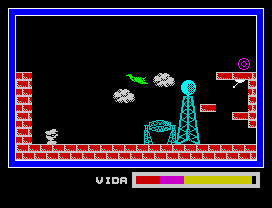
\includegraphics{../screenshots/phantomas-sp1}
\caption{Phantomas (© 1986 Dinamic)}
\label{fig:phantomas}
\end{figure}

\bigskip
Todavía faltaba mucho tiempo para que aprendiera lo que era una interfaz (aún no había aprendido ni tan siquiera a leer) pero ya sabía interpretar algunas letras, curiosamente las que tenían pintadas las teclas OPQA\footnote{En los primeros ordenadores que aparecieron en España en la década de los 80 esta era la combinación de teclas que tenían predefinidos la mayoría de los juegos siendo OP las teclas para moverse de izquierda a derecha y QA para hacerlo de arriba a abajo.}.

\bigskip
Según fui creciendo aprendí a leer y escribir y también a reconocer unos códigos que aparecían al final de las revistas que compraba mi hermano que se llamaban POKES\footnote{Instrucción en lenguaje BASIC que graba un valor en una determinada dirección de memoria.}, estos códigos hacían que, introduciéndolos a la hora de cargar el juego, pudiera tener vidas infinitas, la habilidad de atravesar paredes o la capacidad de ser invisible a los enemigos. Estos trucos permitían a un niño torpe a los mandos, como lo era yo, el poder terminar los dificilísimos juegos de la época.

\bigskip
Pasaron algunos años y ya en el colegio muchos amigos tenían consolas de videojuegos en las que metías un cartucho e instantáneamente estabas jugando a juegos increíbles con una paleta de colores que raro era que no provocara ataques epilépticos. Mientras mis amigos solo tenían que introducir el cartucho y empezar a jugar yo tenía que esperar 5 interminables minutos mientras escuchaba sonidos estridentes y cruzar los dedos por que no apareciera el fastidioso TAPE ERROR que se podía intentar solucionar girando un tornillo llamado 'azimut' con un destornillador que curiosamente aún poseo. 

\bigskip
Quizá fue ahí donde empecé a sufrir los problemas de la usabilidad, yo girando un tornillo sin saber a ciencia cierta el por qué y mis amigos el mayor problema que tenían era que a veces tenían que dar un soplido fuerte a la ranura del cartucho.

\bigskip
Mucho mas tarde entró en mi casa un flamante Pentium 166 MMX con Windows 95 OSR2 y esto era otra cosa, tenía ventanas, podía escribir documentos con formato y el primo de un conocido tenía un programa te marcaba en rojo los errores ortográficos de los trabajos del colegio. De hecho ese mismo tío tenía un CD llamado Encarta donde había toda una enciclopedia metida dentro, solo tenías que escribir una palabra y al momento aparecía su definición con fotografías y todo.

\bigskip
Estábamos ya a mediados de 1996 y se empezaba a hablar de Internet, era como aquella Encarta pero sin CD, el futuro nuevamente había llegado y todo el dinero invertido en una grabadora de CD se iba al garete, junto con las horas mantenidas cruzando los dedos y sin tocar el ordenador para que fallara la grabación, todo estaba en Internet, y si no estaba ahí poco tardaría en estarlo.

\bigskip
Así que cogí los ahorros de mi paga semanal y me compré un módem para puerto serie de 33.000 Baudios de segunda mano. Aún hoy no tengo claro lo que significaba la palabra baudio. Conecté el módem metí uno de los múltiples de CDs de conexión a Internet que regalaban por aquel entonces con las revistas, le di a conectar y ahí estaban de nuevo las largas esperas escuchando ruidos estridentes igual que unos años antes.

\bigskip
A base de curiosear como buen aspirante a ingeniero vi escondido en las opciones una casilla que decía 'Silenciar altavoz', ¿como podía ser que millones de personas estuvieran soportando esos ruidos estridente para conectarse por no saber marcar una casilla? Algo raro pasaba ya que la opción estaba ahí pero nadie la pulsaba.

\bigskip
Pasaron los años, los sistemas se fueron haciendo mas complejos y me di cuenta que según más opciones tenían los dispositivos más perezosos se volvían los usuarios. Mi vecino sin ir más lejos por no configurar su televisor tenía TVE2 en el canal 4 de su televisor ¿era yo el único que encontraba eso chirriante? Quizá no, pero como he ido descubriendo hay diferentes tipos de personas, están los que pueden pasar meses alumbrando el pasillo con el teléfono móvil y los que simplemente llegan y cambian la bombilla. 

\bigskip
Por eso creo que es nuestro deber como ingenieros, ya que tenemos la capacidad de detectar necesidades de las personas y ponerles solución, ya que tenemos el conocimiento y la capacidad de cambiar el mundo. Podemos dejar silenciado por defecto el volumen del altavoz de un módem o bien podemos inventar una bombilla que nos avise de cuántas horas de vida le quedan.

\bigskip
Y por encima de todo, tenemos la capacidad de hacer sencillas las cosas más complejas que es la premisa básica de la usabilidad. No le puedes pedir a tu madre que entienda la incongruencia de pasarte una foto de tu sobrina en e-mail con un documento de Word adjunto y la foto pegada dentro de dicho documento, tienes que ponérselo fácil para que no haga esas barbaridades.

\bigskip
Por eso es tan importante que los que tenemos los conocimientos los invirtamos en ayudar a mejorar los interfaces. Una gran parte de los usuarios no se va a dar cuenta de los problemas de usabilidad ya que muchas veces dicha usabilidad es subconsciente.

\section{Motivación}

Como ya sabemos Internet ha tenido un carácter académico desde prácticamente su nacimiento y por ello las mayores innovaciones y casi todo su enfoque ha salido de estos ámbitos previos a la democratización de la red y el acceso global a Internet. Es impensable concebir hoy día la enseñanza sin hacer uso de Internet y puede que en un futuro no muy lejano la totalidad de la enseñanza se imparta a través de la red.

\bigskip
Pero un uso tan generalizado es inconcebible sin una interfaz adecuada que sea amigable, sencilla e incluso atrayente y es por eso que muchas empresas gastan millones de dólares en mejorar las interfaces. 'La usabilidad ha venido para quedarse' \cite{jakonielsen}.

\bigskip
Tras la implantación definitiva de la plataforma \textbf{Prado2} por parte de la \textit{Delegación de la Rectora para la Universidad Digital} se han venido sucediendo críticas por parte tanto de alumnos como profesores a las carencias de la plataforma, esto, junto a los insuficientes recursos con los que cuenta el CEVUG para dar un servicio adecuado ha hecho que una plataforma potente y consolidada como es moodle genere rechazo ya que como bien apuntaba Steve Krug: 'Si un sistema no es usable nadie lo querrá usar' \cite{stevekrug}


\section{Estructura del proyecto}


\bigskip
Antes de pasar a detalles más técnicos, me gustaría detallarte lo que te vas a encontrar en este proyecto:

\begin{itemize}
  \item En el \textit{capítulo 1} (\textbf{Introducción}), vas a encontrar el texto que estas leyendo ahora mismo así como una breve historia de las plataformas utilizadas por la Universidad de Granada.
  \item En el \textit{capítulo 2} (\textbf{Objetivos}), detallo de forma algo más concreta los objetivos determinados que se quieren cumplir con este proyecto.
  \item En el \textit{capítulo 3} (\textbf{Metodología}), la planificación y desarrollo de cada uno de los análisis del proyecto.
  \item En el \textit{capítulo 4} (\textbf{Resultados}), detallar todos los resultados obtenidos.
\end{itemize}

\bigskip
Una vez estén realizadas las partes descriptivas y de resultados quedarán solo por añadir la parte final; el \textit{capítulo 5} (\textbf{Conclusiones}) en el que se indicarán las diferentes conclusiones a las que se han llegado así como las recomendaciones tanto de carácter urgente como opcionales.

\bigskip
Para finalizar se incluye un anexo con una selección de los comentarios dados a la encuesta así como el código fuente de los scripts desarrollados.

\section{Breve historia de los MOOC}

Quizá la primera referencia a un sistema de enseñanza online lo tenemos en el número de septiembre de 1934 de la revista ‘Everyday Science and Mechanics‘, el presidente de la Universidad Northwestern, Walter Dill Scott decía que ``la universidad, dentro de veinticinco años, será un concepto de aspecto diferente. En lugar de concentrar al profesorado y a los estudiantes alrededor de un campus, los conocimientos ‘viajarán por el aire’. El curso se llevará a cabo, en gran medida, a través de sonido e imágenes; la radiodifusión, la televisión y el telefax ampliarán el ámbito de una biblioteca, y las investigaciones podrán ser llevadas a cabo, por los académicos, a grandes distancias''\cite{art_12}.

\bigskip
Años mas tarde, en 1988, Sir Isaac Asimov expresaba la aparición de los MOOC en un video video titulado "Su visión hacia el futuro" pero no fue hasta finales de los años 90 cuando el MIT comenzó la iniciativa OpenCourseWare que fue la primera aproximación real hacia la enseñanza digital.

\bigskip
En el año 2002 comienza el desarrollo de la plataforma moodle, cuando aún se hablaba de e-learning ya que el término MOOC fue acuñado en 2008 por Dave Comier de la University of Prince Edward Island.

\bigskip
En 2011, más de 160.00019 personas repartidas por todo el mundo se matricularon en un curso de Inteligencia artificial ("Introduction to Artificial Intelligence") ofrecido por Sebastian Thrun y Peter Norvig en la Universidad de Stanford.

\bigskip
El 2012 se reconoce como el año a partir del cual los MOOC tienen su auge, el New York Times, publica un artículo denominado "El año de los MOOC", acreditando que en este año el nuevo "formato" educativo ha sido utilizado por "el gran público".

\section{Historia de las plataformas online de la UGR}

Cuando en el año 2013 comencé mis estudios en la Universidad de Granada me sorprendió el encontrarme con varias plataformas de docencia online, prácticamente una para cada departamento y todas ellas tenían puntos buenos y puntos a mejorar.

\bigskip
En mi segundo año se estaba empezando a implantar Prado2 que venía a resolver el problema de la fragmentación, como ya hemos dicho cada profesor era libre de elegir el sistema que más le gustara pero, a cambio de esta libertad, los alumnos teníamos que aprender a usar todas y cada una de las distintas plataformas.

\bigskip
Quizá no todos los estudiantes de la UGR han tenido que lidiar con esta situación, ya que compañeros de otras facultades sólo han conocido el Tablón de Docencia y a lo sumo SWAD antes de pasar al nuevo Prado2, pero los estudiantes de la ETSIIT, por el carácter de los estudios que tenemos si hemos sido 'conejillos de indias' de todas estas plataformas.

Quisiera agradecer a los responsables de las diferentes departamentos su ayuda a la hora de conocer la historia de cada una las plataformas.

\subsection{Tablón de docencia}

Fue desarrollado por el CSIRC pero, aunque hemos intentado ponernos en contacto con ellos para conocer la historia de esta plataforma, no hemos recibido respuesta.

\subsection{SWAD (Sistema Web de Apoyo a la Docencia)}

\bigskip
La primera versión de SWAD apareció en septiembre de 1999. A partir de 2005 comenzó a extenderse su uso en la Universidad de Granada. La aplicación fue liberada en enero de 2010 bajo licencia GNU Affero General Public License, versión 3.

\bigskip
SWAD fue desarrollado por el profesor de la UGR Antonio Cañas Vargas utilizando de forma exclusiva lenguaje C.

\bigskip
En 2010 el sistema era usado por 1.100 profesores y 35.000 estudiantes. En 2011 la cantidad ascendía a 2.000 profesores y 60.000 estudiantes en 2.800 asignaturas.

\bigskip
En febrero de 2016 la instalación de SWAD en la Universidad de Granada albergaba 419 titulaciones (incluyendo grado y posgrado) con 7114 asignaturas, 110057 estudiantes y 3304 profesores.

\bigskip
SWAD está disponible actualmente en 9 idiomas y se utiliza en la Universidad de Granada y en el portal OpenSWAD.org.


\subsection{PRADO}

La primera versión de Prado2 fue publicada en 2014 por el CEVUG, al estar basada en moodle su código está íntegramente desarrollado en PHP, aunque solicitamos información al CEVUG no nos han proporcionada los datos de sus desarrolladores así la historia de su desarrollo.

\subsection{DECSAI}

La primera versión fue publicada en 2003 y fue desarrollada por Pablo Orantes Pozo y Miguel García Silvente utilizando el lenguaje PHP. En 2010 se desarrolló una segunda versión que corresponde casi exactamente con la actual.

\bigskip
El desarrollo de esta plataforma web ha tenido tres etapas: 
La versión 3.0 disponible a partir de finales de 2013 emplea la plantilla institucional facilitada por la Oficina Web de la Universidad de Granada y es realizada por Pablo Orantes Pozo bajo la dirección de Miguel García Silvente.

\bigskip
La versión 2.0 corresponde a un rediseño y programación casi completo realizado por Pablo Orantes Pozo bajo la dirección de Miguel García Silvente.

\bigskip
La versión 1.0 (2004-2009) se realizó bajo la coordinación de Miguel García Silvente, Francisco G. Raúl Pérez Rodríguez y Gracia Pérez López.

\bigskip
Las tareas de programación de la versión 1.0 fueron realizadas por: Carlos Cano Gutiérrez, Juan Gómez Romero, Pedro J. Magaña Redondo y Gracia Pérez López, en las modificaciones posteriores participó Andrés Cano Utrera.

\subsection{TUTOR}
Esta plataforma web de apoyo a la enseñanza universitaria ha sido desarrollada en el seno de tres Proyectos de Innovación Docente. Lo realizado en cada uno de ellos se indica en la segunda sección de la página \url{https://tutor.ugr.es/functions/index.php/idop_info}. La primera versión fue publicada en 2004 y fue desarrollada por Álvaro López Martínez, Roberto F. Arroyo Moreno y Miguel J. Hornos Barranco, el lenguaje de programación utilizado fue PHP.

\chapter{Objetivos y Temporización}


El objetivo máximo de este proyecto es realizar un análisis detallado de la plataforma Prado2 que pueda servir como una herramienta para facilitar el trabajo a los administradores de la misma, ya que la evidente falta de recursos del CEVUG hace que un análisis de dichas características sea poco menos que imposible.

\bigskip
Dicho objetivo es el conjunto de los siguientes objetivos principales:

\begin{itemize}
  \item \textbf{OBJ-1.} Analizar la usabilidad de Prado2.
  \item \textbf{OBJ-2.} Analizar la accesibilidad de Prado2.
  \item \textbf{OBJ-3.} Analizar la seguridad de Prado2.
  \item \textbf{OBJ-4.} Analizar la disponibilidad de Prado2.
  \item \textbf{OBJ-5.} Promover la idea de que los desarrollos bajo software libre en general y en la administración pública en particular ayudan a generar confianza y demuestran compromiso.
  
\end{itemize}

Además como objetivos secundarios tendremos:

\begin{itemize}
  \item \textbf{OBJ-6.} Estudiar la posibilidad de hacer un clon de la instalación actual de Prado2 en un servidor propio.
  \item \textbf{OBJ-7.} Estudiar la posibilidad de desarrollar una herramienta para solventar los problemas de usabilidad de la plataforma. 
  \item \textbf{OBJ-8.} Estudiar la posibilidad de desarrollar una herramienta para solventar los problemas de seguridad de la plataforma. 
   \item \textbf{OBJ-9.} Estudiar la posibilidad de configurar un dispositivo hardware para analizar la seguridad de la plataforma.
\end{itemize}



\section{Alcance de los objetivos}
El fin inmediato de este informe es servir de herramienta a los administradores de la plataforma para que conozcan los fallos más importantes y sugerencias sobre como solucionarlos.
Además el informe resultante se liberará con una licencia libre para que cualquier parte interesada pueda hacer uso las conclusiones y los datos extraídos del análisis.

\section{Interdependencia de los objetivos}

Todos los objetivos son independientes entre sí, pero el primer objetivo (\textbf{OBJ-1}) es el principal motivador de este proyecto, por lo que aún sin representar el desarrollo de ningún trabajo en concreto es el que va a escudar y avalar el desarrollo de los otros. En aspectos más relacionados con la realización del proyecto, el tercer objetivo (\textbf{OBJ-3}) es el que se requerirá solucionar de forma inmediata, ya que impide el correcto funcionamiento del portal. El resto de objetivos serán tratados en mayor o menor medida.

\section{Conocimientos y herramientas utilizadas}

\bigskip
Destacar en los aspectos formativos previos más utilizados para el desarrollo del proyecto los conocimientos sobre Desarrollo de Aplicaciones para Internet para el análisis de usabilidad y accesibilidad, Fundamentos de Ingeniería de Software para el análisis del proyecto, Seguridad en Sistemas Operativos para la parte de seguridad y Servidores Web de Altas Prestaciones para la realización de pruebas desde el punto de vista de disponibilidad y carga de trabajo.

Para la realización de cada una de las partes se han usado multitud de herramientas específicas tales como pueden ser WireShark, ettercap, statusCake, Latex, R, Google Forms y Google SpreadSheets entre otras. 


\section{Temporización estimada}


En la figura \ref{fig:temporizacion1} podemos ver la planificación de tiempos para el desarrollo de este proyecto. 

\begin{figure}[H]
\centering
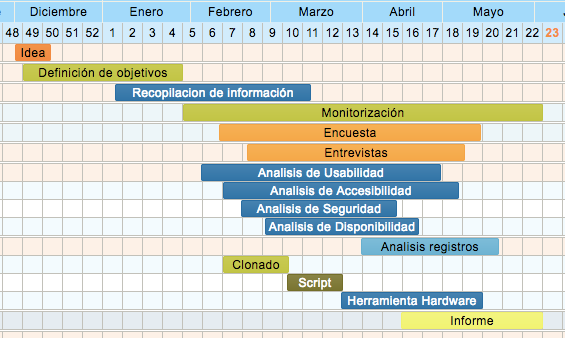
\includegraphics[width=0.8\textwidth]{../screenshots/temporizacion1}
\caption{Diagrama de Gantt con los tiempos estimados para el proyecto}
\label{fig:temporizacion1}
\end{figure}








\chapter{Metodología}

\section{Análisis general de la plataforma}
Se realizó un análisis general de la herramienta para conocer enteramente con qué nos encontramos, en qué plataforma está basada y si se han realizado desarrollos adicionales sobre la misma para adecuarlo a las necesidades de la UGR.

\section{Entrevistas personales}

Para recoger la mayor información posible sobre las opiniones de los usuarios de Prado2 se realizaron una serie de entrevistas personales de carácter informal con profesores, alumnos y administradores y así poder hacer una valoración global del estado actual de la plataforma, teniendo en cuenta a todos los actores implicados en la misma.

\bigskip
Algunas de estas entrevistas incluyeron un test de usabilidad que consistía en pedir a los usuarios que realizaran una tarea sencilla y ver cuánto tiempo tardaban en realizarla. 

\bigskip
Dicha tarea consistía en pedirles cambiar la imagen del perfil de Prado2. El test se basó en el test de usabilidad planteado por Steve Krug en su libro \textit{Don't make me think} \cite{stevekrug} y se pedía que partiendo de una página neutra, como puede ser la pagina de inicio de un buscador, entraran en Prado2 y localizaran desde donde podían cambiar su imagen de perfil.


\section{Encuesta a los usuarios}
Uno de los actores más importantes de cualquier plataforma web son sus usuarios por lo que queríamos conocer de primera mano sus opiniones, para ello se preparó un breve cuestionario online que fue difundido a través de la lista de correo general de la UGR.

\bigskip
La encuesta se realizó con la herramienta \texttt{Google Forms} y estuvo activa desde el 14 de Marzo hasta el 10 de Mayo de 2017, los primeros días se le dio difusión a través de grupos de mensajería y redes sociales. El 21 de Marzo se envió a la lista de correo infoUGR de la Universidad por parte del Tutor y el 23 de Marzo la DEIIT nos hizo el favor de enviarla a la comunidad de estudiantes de la ETSIIT ya que la lista infoUGR al estar en un buzón propio no suele tener la difusión que tienen los mensajes que van a la bandeja de entrada.

\bigskip
Dicho cuestionario constaba de varias preguntas preguntas cerradas de respuesta múltiple, ya que las mismas son más objetivas a la hora de hacer un análisis estadístico, también se incluyeron tres preguntas opcionales de respuesta abierta para que los usuarios pudieran exponer razonadamente sus opiniones.

Las preguntas eran las siguientes:

\begin{enumerate}

  \item \textbf{Selección del tipo de usuario} Se pregunta si el usuario es Estudiante, Profesor u otro tipo de miembro de la comunidad universitario, como por ejemplo, doctorandos.

  		\shadowbox{
\includegraphics[width=0.9\textwidth]{../screenshots/poll/01}}

  \item \textbf{Selección de la titulación} Se pregunta la titulación del usuario, ya que vimos que las opiniones variaban en base a la misma, el listado oficial de titulaciones lo obtuvimos del Portal de Transparencia de la UGR \url{http://transparente.ugr.es/}

  \shadowbox{
\includegraphics[width=0.9\textwidth]{../screenshots/poll/02}}

  \item \textbf{¿Con qué periodicidad accede a Prado2?} Es interesante saber  la periodicidad con la que los usuarios acceden a la plataforma, para además cotejarla con el análisis de los registros de moodle

  \shadowbox{
\includegraphics[width=0.9\textwidth]{../screenshots/poll/03}}

  \item \textbf{Califique las siguientes opciones según sus necesidades} Presentamos al usuario una serie de opciones de la plataforma extraídas de valoraciones personales de varios usuarios, dichas opciones son:

  		\begin{itemize}
  			\item \textbf{Acceso desde dispositivos móviles} La mayor parte de las quejas recibidas antes de empezar este proyecto era la dificultad para acceder desde dispositivos móviles y la falta de una aplicación nativa para dichos dispositivos.
  			\item \textbf{Insignias} Implementación del sistema de insignias de Mozilla Open Badges para otorgar a los alumnos reconocimiento digital de sus cualidades y logros.
  			\item \textbf{Blog de la asignatura} Permitir a las asignaturas mantener un blog dentro de la plataforma, dicho blog solo está accesible para los alumnos de la asignatura.
  			\item \textbf{Blog de los alumnos} Permitir a los alumnos mantener un blog dentro de la plataforma, las publicaciones de dicho blog se pueden configurar para que sean visibles solo para otros alumnos de la misma asignatura o para todos los usuarios de la plataforma.
  			\item \textbf{Mensajería interna} Se debe permite la comunicación entre profesores y alumnos sin salir de la misma.
  			\item \textbf{Estadísticas de uso} Permitir a los alumnos y profesores acceder a las estadísticas de uso de la plataforma.
  			\item \textbf{Calificaciones} Permitir a los alumnos acceder a las calificaciones de sus tareas y exámenes de la asignatura.

		\end{itemize}

		\shadowbox{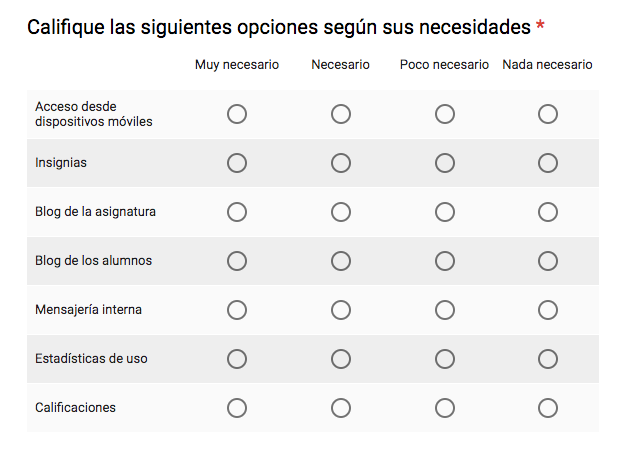
\includegraphics[width=0.9\textwidth]{../screenshots/poll/04}}


  \item \textbf{Actividades y recursos} Presentamos la lista de actividades que puede crear un profesor en una asignatura para ver cuáles son las más utilizadas (las actividades marcadas con * son actividades desarrolladas expresamente para Prado2).


        \begin{itemize}
            \item \textbf{Auto-selección de Grupo *} Esta actividad permite a los alumnos seleccionar su grupo de prácticas al inicio del curso.

            \item \textbf{Base de datos}: Les permite a los participantes crear, mantener y buscar dentro de un banco de entradas de registros.

            \item \textbf{Chat}: Les permite a los participantes tener una discusión sincrónica en tiempo real.

            \item \textbf{Consulta}: Un profesor hace una pregunta y especifica una variedad de respuestas de opción múltiple.

            \item \textbf{Control de Asistencia *}: Esta actividad permite controlar la asistencia a clase.

            \item \textbf{Cuestionario}: Permite al profesor diseñar exámenes, que pueden ser calificados automáticamente.

            \item \textbf{Encuestas predefinidas}: Para recolectar datos de los estudiantes, para ayudar a los profesores a conocer sus alumnos y reflexionar sobre su enseñanza.

            \item \textbf{Foro}: Permite a los participantes tener discusiones asincrónicas.

            \item \textbf{Glosario}: Permite a los participantes crear y mantener una lista de definiciones, a semejanza de un diccionario

            \item \textbf{Herramienta Externa}: Permite a los participantes interactuar con recursos y actividades de enseñanza compatibles con LTI en otros sitios web.

            \item \textbf{Paquete SCORM}: Permite que se incluyan paquetes SCORM como contenido del curso.

            \item \textbf{Lección}: Para proporcionar contenido en formas flexibles.

            \item \textbf{Taller}: Habilita la evaluación por pares.

            \item \textbf{Tarea}: Permite a los profesores calificar y hacer comentarios sobre archivos subidos y tareas creadas en línea y fuera de línea

            \item \textbf{Wiki}: Una colección de páginas web donde cualquiera puede añadir o editar.

            \item \textbf{Archivo}: Son materiales que podemos poner a disposición del alumnado en diferentes formatos: documentos de texto, imágenes, vídeos, audios, archivos comprimidos, etc.

            \item \textbf{Carpeta}: Se utilizan para poner a disposición del alumnado múltiples archivos agrupados en un ítem.

            \item \textbf{Clase grabada (GA3) *}: Esta actividad permite subir una clase grabada con el sistema GA3 para su posterior visualización.

            \item \textbf{Etiqueta}: Se utilizan para insertar pequeñas secciones de texto, imágenes o elementos multimedia entre los distintos bloques de contenido del curso.

            \item \textbf{Libro}: Recursos multi-página con aspecto similar a un libro. Los maestros pueden exportar sus Libros como paquete IMS (el administrador debe permitir que el rol de maestro pueda exportar IMS)

            \item \textbf{Página}: Permiten añadir contenido directamente en Moodle, mediante el editor de texto disponible.

            \item \textbf{Paquete de contenido IMS}: Es un tipo de formato de archivo estándar basado en una serie de especificaciones que facilitan la reutilización de contenidos en distintos sistemas sin necesidad de convertirlos a otro formato.

            \item \textbf{URL}: Permite agregar un enlace a un sitio web.

        \end{itemize}
		\shadowbox{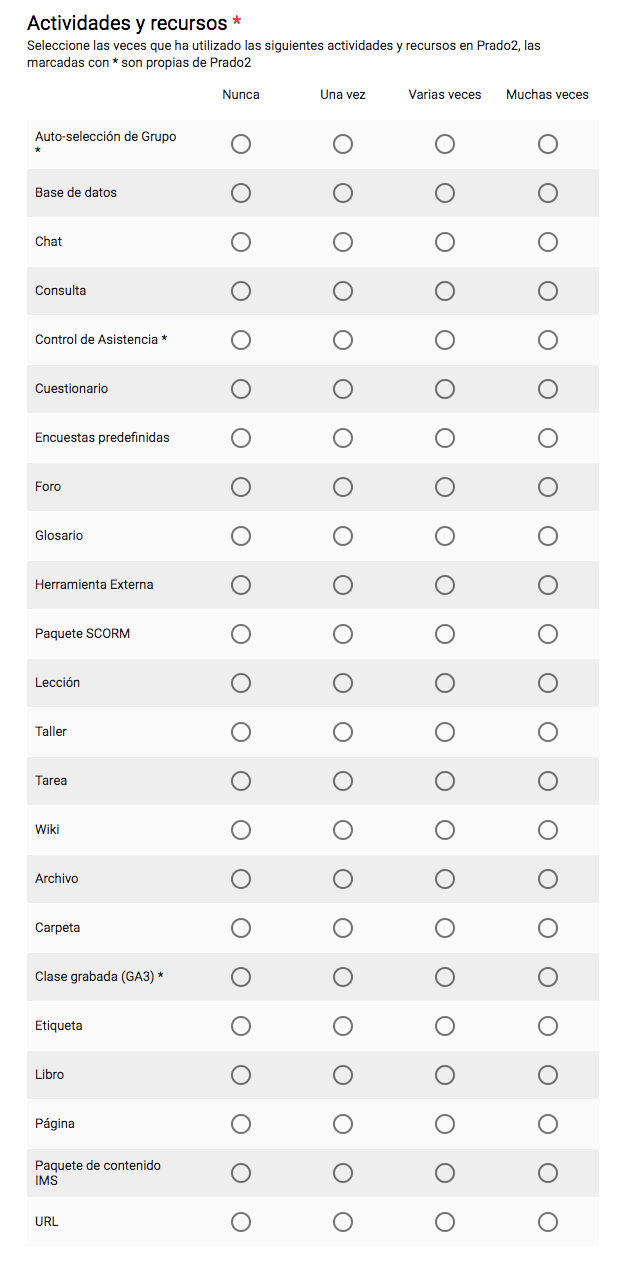
\includegraphics[width=0.9\textwidth]{../screenshots/poll/05}}


  \item \textbf{¿Cómo calificaría Prado2?} Presentamos al usuario los aspectos mas importantes para calificar la plataforma, dichos aspectos son:

  		\begin{itemize}
  			\item \textbf{Usabilidad} Define si un sistema es sencillo de usar, facilita la lectura, presenta funciones y menús sencillos, por lo que es cómodo su uso.
  			\item \textbf{Accesibilidad} Grado en el que todas las personas pueden utilizar el servicio, independientemente de sus capacidades técnicas, cognitivas o físicas.
  			\item \textbf{Seguridad} Define lo robusto que es un sistema frente a ataques informáticos.
  			\item \textbf{Disponibilidad} Disponibilidad: Medida que indica cuanto tiempo está disponible el sistema y lo resistente que es frente a caídas.
  			\item \textbf{Valoracion General} La valoración de la plataforma en su conjunto.

		\end{itemize}

    \shadowbox{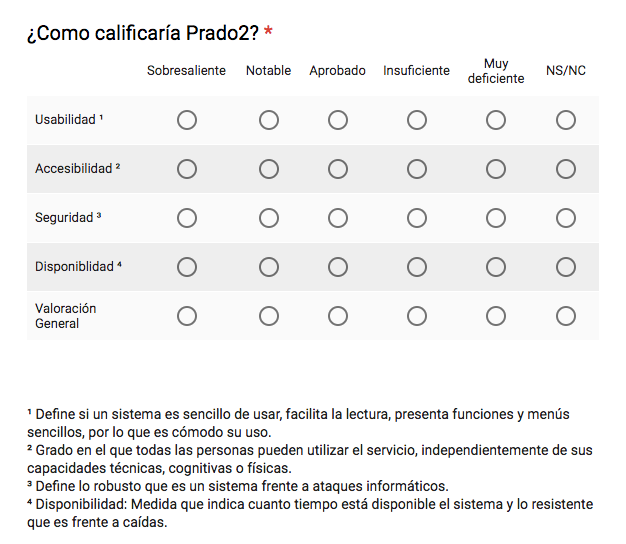
\includegraphics[width=0.9\textwidth]{../screenshots/poll/06}}

  \item \textbf{¿Con cúales de las siguientes plataformas de la UGR ha trabajado?} Presentamos al usuario una lista con las plataformas de docencia más importantes de la UGR:

  		\begin{itemize}
  			\item DECSAI
            \item Tutor
            \item SWAD
            \item Tablón de docencia
            \item Prado 1 - CEVUG (Moodle)
            \item Prado 2 (Moodle)
            \item Otro
		\end{itemize}

  \shadowbox{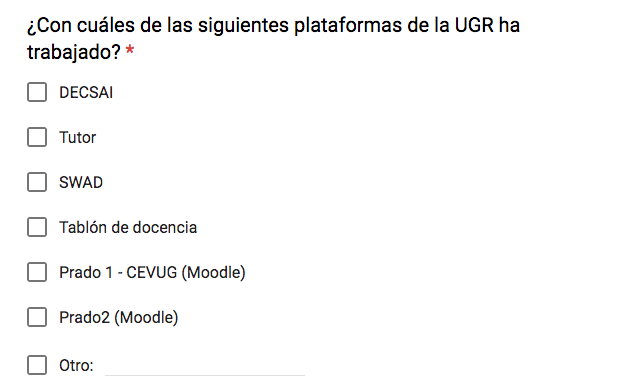
\includegraphics[width=0.9\textwidth]{../screenshots/poll/07}}

  \item \textbf{De las siguientes plataformas de la UGR ¿Cuál prefiere?} Presentamos al usuario una lista con las plataformas de docencia más importantes de la UGR:

  		\begin{itemize}
  			\item DECSAI
            \item Tutor
            \item SWAD
            \item Tablón de docencia
            \item Prado 1 - CEVUG (Moodle)
            \item Prado 2 (Moodle)
            \item Otro
		\end{itemize}

    \shadowbox{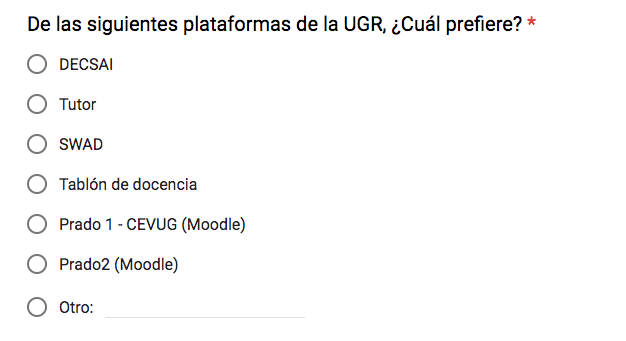
\includegraphics[width=0.9\textwidth]{../screenshots/poll/08}}

  \item \textbf{¿Ha encontrado algún error que debería ser subsanado en Prado2?} Permitimos al usuario expresar su opinión detallada.

  \shadowbox{
\includegraphics[width=0.9\textwidth]{../screenshots/poll/09}}


  \item \textbf{Indique si hay alguna función adicional que le gustaría ver en Prado2} Permitimos al usuario expresar su opinión detallada.

  \shadowbox{
\includegraphics[width=0.9\textwidth]{../screenshots/poll/10}}

  \item \textbf{Indique cuál es la funcionalidad que más le gusta de Prado2} Permitimos al usuario expresar su opinión detallada.

  \shadowbox{
\includegraphics[width=0.9\textwidth]{../screenshots/poll/11}}

  \item \textbf{E-mail} Permitimos al usuario proporcionarnos su dirección de e-mail para futuros contactos.

  \shadowbox{
\includegraphics[width=0.9\textwidth]{../screenshots/poll/12}}

  \item \textbf{Comentarios adicionales} Permitimos al usuario expresar su opinión detallada
  
  \shadowbox{
\includegraphics[width=0.9\textwidth]{../screenshots/poll/13}}

\end{enumerate}

\section{Análisis de registros propios de la plataforma}

La plataforma moodle provee de mecanismos para registrar el uso de la misma en diversas tablas de registro, particularmente la versión utilizada usa la tabla \texttt{mdl\_log} (ver figura \ref{logtable}) para almacenar los registros de acceso de los usuarios. Cabe indicar que a partir de la versión 2.7 de moodle la tabla\texttt{mdl\_log}  ya no se utiliza y ha pasado a marcarse como obsoleta\cite{art_09} en favor de la tabla \texttt{mdl\_logstore\_standard\_log}.

Dicha tabla mantiene un registro de todas las interacciones de los usuarios en la página así que podemos extraer información interesante como el tiempo medio de la plataforma por parte de los usuarios o que actividades tienen mas uso. 

Como la tabla contenía información personal como puede ser el identificador del usuario y su dirección ip se optó por diseñar una consulta SQL que retornara los datos usando anonimizando los datos sensibles mediante una función hash.

\begin{figure}\centering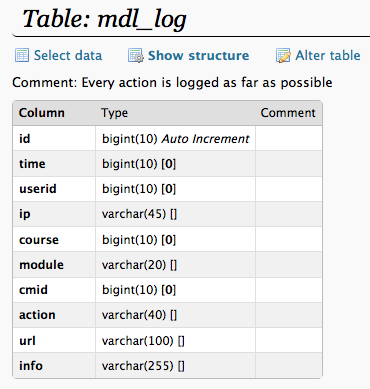
\includegraphics[width=0.8\textwidth]{../images/logtable}\caption{Tabla de log}\label{logtable}\end{figure}

\begin{lstlisting}
SELECT
    id, time, MD5(userid), MD5(ip), MD5(course), module, cmid, action, url, info
FROM
    mdl_log
\end{lstlisting}


Tras una reunión en el CEVUG con los responsables de Prado2 mantenida el 23 de Marzo de 2017 donde nos transmitieron su apoyo y colaboración acordamos realizar una petición formal de datos al CSIRC.

Una vez definida la consulta se realizó al CSIRC una petición formal de datos. Tras varios intentos infructuosos de realizar la petición de forma telemática por parte del tutor se optó por realizarla de forma presencial en papel.

El día 23 de Mayo nos remitieron desde el CEVUG una muestra de los datos de 2014 para ver si los datos eran correctos antes de darnos en fases los datos completos. La primera fase correspondiente a los datos de 2015 los tuvimos disponibles el 1 de Junio en un fichero csv\footnote{Los archivos CSV (del inglés comma-separated values) son un tipo de documento para representar datos en forma de tabla en las que las columnas se separan por comas.} de 500 megabytes conteniendo 3.119.094 registros.


\begin{lstlisting}
SQL> select  /*csv*/ l.id,l.time,rawtohex(sys.DBMS_OBFUSCATION_TOOLKIT.MD5(INPUT_STRING => l.userid)) userid_md5,rawtohex(sys.DBMS_OBFUSCATION_TOOLKIT.MD5(INPUT_STRING => l.ip)) ip_md5 ,l.course, substr(c.idnumber,0,14) course_code,substr(c.idnumber,0,3) tit, substr(c.idnumber,5,2) plan, substr(c.idnumber,8,2) cea, l.module,l.cmid, l.action, l.url, l.info from p_log l, p_course c where (l.course=c.id and l.userid>10 and REGEXP_LIKE(c.idnumber, '^[0-9]') and  l.time>1420070400 and l.time<1451606400);

\end{lstlisting}

Con los datos recogidos y basándonos en el excelente articulo\cite{art_02} de James Ballard que aunque se centra en en el análisis de la nueva tabla de log de las versiones 2.7 y superiores nos sirvió de base con la que crear una serie de consultas en lenguaje R que procesara los datos para sacar conclusiones de los mismo. Dichas consultas se adjuntan en el anexo.

\section{Análisis de usabilidad de la plataforma}

Una vez obtenida la información
Para esta tarea primeramente se tuvieron en cuenta toda la información extraída de las entrevistas personales y se procedió a ver si realmente era usable.

\section{Análisis de accesibilidad de la plataforma}

Se analizó mediante diversas herramientas si la plataforma era accesible, esta tarea la ampliamos para que incluyera tanto la accesibilidad para personas como discapacidad como la accesibilidad desde dispositivos móviles y el uso en otros idiomas.

\section{Análisis de seguridad}

Para analizar la seguridad de la plataforma se realizó una auditoría para ver que información sensible se podía extraer de la misma. Para la misma se analizaron las vulnerabilidades específicas de la versión instalada mirando en distintos repositorios de exploits así como en el propio listado de vulnerabilidades de moodle que se puede encontrar en \url{https://moodle.org/security/}

\bigskip
Asimismo se diseñó un ataque dirigido de secuestro de sesión \textit{(session hijacking)} y se intentaron robar las variables de sesión de moodle del tutor bajo su consentimiento expreso.

\section{Análisis de disponibilidad}

Para el análisis de  disponibilidad de la plataforma se optó por monitorizar la web mediante la herramienta StatusCake \cite{statuscake}.

\bigskip
Dicha herramienta va lanzando continuamente peticiones de conexión a la página desde diferentes centros de datos a lo largo del mundo y va registrando el tiempo que tarda en responder y el tipo de respuesta para saber si la página está operativa o caída.

\bigskip
Una de las cosas interesantes de esta herramienta es que se pueden configurar varios tipos de avisos por lo que si la plataforma sufría una interrupción del servicio nos lo notificaba por e-mail, así como nos notificaba cuando volvía a estar operativo.



\section{Clonado de la plataforma}

Con la información obtenida en en análisis general se planteó la posibilidad de poner un funcionamiento un clon de la plataforma en un servidor propio, en un primer contacto los administradores nos dijeron que lo mismo no sería posible por lo que se optó por realizar una instalación de la misma versión de moodle que hay actualmente en prado así como la plantilla utilizada haciendo las mínimas adaptaciones necesarias para que fuera lo más parecido posible a la instalación actual.

\section{Realización de scripts GreaseMonkey}

Para solventar los problemas de seguridad y accesibilidad se planteó realizar una serie de scripts en formato GreaseMonkey que mediante Javascript pudiera hacer los cambios mínimos para:

  		\begin{enumerate}
  			\item Forzar que la página se sirva mediante el protocolo https.
            \item Realizar simples cambios estéticos para mejorar la usabilidad.
        \end{enumerate}

\section{Herramienta hardware para robo de sesiones}

A modo de ejercicio práctico para ver el alcance de la seguridad de la plataforma se propuso crear un dispositivo hardware para cazar credenciales de usuarios a modo de honeypot utilizando un viejo router instalando el firmware OpenWRT \cite{openwrt} e instalando las herramientas necesarias para obtener los identificadores de sesión de los clientes conectados.




\chapter{Resultados}

\section{Análisis general de la plataforma}

La plataforma Prado usa la 2.6.4 de moodle aunque la última versión estable a 15 de mayo de 2017 es la 3.3. La rama 2.6 dejó de recibir actualizaciones de soporte hace 2 años. Para conocer la versión de prado se puede consultar la url \url{http://prado.ugr.es/moodle/lib/upgrade.txt}.

\bigskip
Prado2 usa como plantilla el tema Archaius \cite{moodletheme}, desarrollada por el programador colombiano Daniel Múnera Sánchez. Podemos ver la versión de la plantilla accediendo a \url{http://prado.ugr.es/moodle/theme/archaius/README.md} viendo que la versión instalada es del 11 de agosto de 2014, cuando dicho tema tiene versiones mas actualizadas que solucionan diversos problemas.

\bigskip
Nos pusimos en contacto con el desarrollador de la plantilla, y muy amablemente nos contestó a todas las dudas que teníamos sobre la misma. También nos confirmó que había abandonado el desarrollo de la plantilla por falta de tiempo con lo que no habrá más actualizaciones de la misma.

\bigskip
Al acceder a la url \url{http://prado.ugr.es/} nuestro navegador descargará un archivo index.html (ver figura \ref{redireccionhttp}) que le dirá al navegador que tiene que hacer una nueva petición para descargar la web desde el subdirectorio /moodle/, las redirecciones http están desaconsejadas y hay otras formas de resolver este problema utilizando una única petición htt, por experiencia propia esto deja entrever que se partió de una instalación rápida desempaquetando el fichero comprimido de moodle y empezando a trabajar desde ahí. Se podría entender que se ha dejado para dejar la referencia a que se está usando el paquete moodle pero se han eliminado todas las referencias a la misma, incluso los enlaces a su licencia cosa a la que obliga la GPLv3 que es la licencia de moodle.

\bigskip
Curiosamente Ágora \url{http://pefc5.ugr.es} que es la instalación de moodle que utilizan en la facultad de psicología resuelve esto con una redirección 302

\bigskip
En cuanto al motor de base de datos, desde el CEVUG nos comentaron que utilizaban Oracle por requerimiento del CSIRC, pues no daban soporte a ningún otro motor de base de datos y que habían que tenido que realizar diversas adaptaciones al código de moodle para que funcionara sobre este motor. Tras la recepción de los datos por parte del CEVUG analizando la consulta que lanzaron para obtener los datos pudimos certificar que efectivamente estaban usando Oracle pues la consulta hacía uso de funciones propias de Oracle pero que moodle soporta de forma nativa 4 motores de base de datos: MySQL, PostgreSqL, MSSQL y Oracle por lo que suponemos que las adaptaciones serían para automatizar la creación de cursos, alumnos y profesores.  


\begin{figure}
\centering
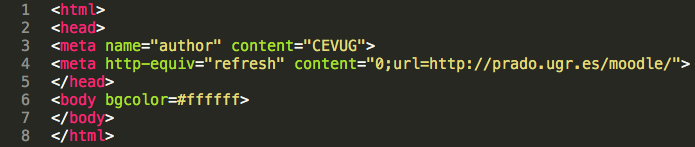
\includegraphics[width=1.0\textwidth]{../screenshots/redireccionhttp}
\caption{Redireccion HTTP al acceder a http://prado.ugr.es}
\label{redireccionhttp}
\end{figure}

\bigskip
Las versiones antiguas de moodle utilizaban la librería YUI desarrollada por Yahoo cuyo desarrollo se abandonó el 29 de agosto de 2014 \cite{art_01} y a partir de la 2.9 se comenzó a migrar a la librería jQuery. Aunque moodle 2.6 utiliza YUI la plantilla Archaius usa varias funciones de la librería jQuery 1.10.2 \url{https://prado.ugr.es/moodle/theme/jquery.php/core/jquery-1.10.2.min.js} que fue liberada el 3 de Julio de 2013 y que teniendo en cuenta que la librería está ya por su versión 3.2 vemos que está claramente obsoleta.

\bigskip
Se está utilizando Apache como servidor HTTP, notar que se oculta su versión haciéndolo mas seguro ante posibles ataques dirigidos, esto es un acierto.

\bigskip
El servidor tiene instalada la versión 5.4.45 que fue liberada el 3 de septiembre de 2015 y que como podemos ver en \url{http://php.net/supported-versions.php} ya no está soportada. En este caso hay dos problemas, por un lado el usar una versión tan anticuada de PHP y por otra no ocultar la versión, siendo muy fácil encontrar vulnerabilidades para dicha versión.

\section{Entrevistas personales}

Como ya hemos comentado se hicieron una serie de entrevistas informales en las que simplemente se anotaban los puntos de vista de los usuarios así como sus quejas y sugerencias y se culminaba con un pequeño test de usabilidad consistente en pedir a los usuarios que cambiaran su foto de perfil de Prado2. En el test participaron cerca de 30 personas, tanto profesores y usuarios de Prado2 como gente externa que nunca había visto la plataforma.

\bigskip
Para cambiar la imagen de perfil de prado dos la ruta correcta a seguir es: Administración - > Editar Perfil - > Imagen del Usuario y aunque puede parecer sencillo nadie bajó del minuto y medio mientras probaba erráticamente en varios sitios, hubo un estudiante del Grado en Ingeniería Informática que tardó más de 4 minutos.

\bigskip
Todos los usuarios repetían básicamente el mismo patrón, como se les pedía que cambiaran la imagen del perfil lo primero que hacían era hacer click en la imagen para ver si salía alguna opción de editar, lo que deja entrever lo lejos que está la plantilla actual del uso real que hacen los usuarios. 

\bigskip
Además los distintos usuarios nos hicieron notar los siguientes problemas y/o carencias con los que se habían encontrado:

\begin{enumerate}

\item No se puedes desmatricular de asignaturas de otros cursos o de las que el alumno ha cambiado de grupo

\item Aunque se entre en inglés hay muchas cosas que aparecen en castellano, de hecho están mezclados ambos idiomas

\item La ventana de solicitud de contraseña de prado2 (el IDP del CSIRC) coge la configuración de idioma del navegador del usuario en lugar de la que viene de prado, esto hace que si por ejemplo tu navegador está en inglés pero tu estás mostrando prado en español, al acceder al IDP la ventana se mostrará en inglés.

\item Hay que bajar los materiales de la asignatura uno a uno en lugar de dar una opción para descargar todo el conjunto

\item Si se está navegando por la miga de pan se llegan a mostrar unos listados de asignaturas con mas de mil registro haciendo inusable el seleccionar alguna

\item El menú superior de asignaturas es inusable por los profesores pues no saben a ciencia cierta a que asignatura están accediendo hasta que han hecho click ya que muchas asignaturas comparten nombre simplemente cambiando los profesores

\item No se notifican los cambios y/o novedades en la plataforma, encontrando a veces que algo que funcionaba de una determinada manera ha cambiado, provocando confusión.

\item Si un alumno contiene un carácter no ascii como pueden ser vocales acentuadas o una "ñ", a la hora de descargar los trabajos de dicho alumno la codificación del archivo será incorrecta y al desempaquetar el archivo .zip en sistemas windows aparece una carpeta vacía (en sistemas Linux no hay problema). En este caso el profesor recibió una queja del alumno por que no le habían calificado una serie de ejercicios y el profesor estuvo haciendo comprobaciones en varios sistemas y lo puso en conocimiento del CSIRC, donde le aseguraron que era problema de su equipo. 

\item En determinados listados no aparecen barras de desplazamiento horizontal por lo que aparece la información cortada, en otros listados al contrario dichas barras son tan largas que en numerosas  ocasiones se ha perdido la localización espacial de la fila y se ha puntuado al alumno incorrecto.

\item Hay diferentes vistas de la ventana "Mis cursos" con la consecuente confusión

\item No se notifica a los usuarios cuando hay material nuevo o modificado obligando a comprobar periódicamente el material uno a uno.

\item Las calificaciones finales no se muestran aunque el profesor las publique.

\item A la hora de mostrar las calificaciones salen trozos de pruebas ocultas de otros cursos y otros grupos sin rellenar.

\item No se notifica la convocatorias de exámenes.

\item El sistema de mensajería es complicado de encontrar y mucho mas complicado de usar, primeramente el profesor ha de marcar uno a uno los alumnos no habiendo una opción para seleccionarlos todos, luego en lugar de aparecer un botón que ponga "Enviar mensaje" aparece un desplegable cuya única opción es "Enviar mensaje" (ver imagen \ref{fig:pantallazoPradoenviarMensaje}), al darle a esa opción pasamos a una ventana donde podemos redactar el mensaje aunque las opciones de insertar elementos no funcionan correctamente. En la parte inferior de ese mensaje vemos que aparece de nuevo toda la lista de alumnos sin respetar los que se habían marcado previamente. Al enviar el mensaje el profesor no recibe una copia pese a haberse marcado, con lo que no puede comprobar que efectivamente se está enviado el correo a todos los alumnos. El editor de mensajes no deja copiar/pegar con el botón derecho del ratón aunque si que deja hacerlo mediante atajos de teclado y por último y no menos importante no permite editar el asunto del mensaje. Si además sucede algún problema al enviar mensajes a los alumnos nos podemos encontrar con un críptico mensaje de error como el de la figura \ref{fig:pantallazoPradoMensaje2} que reza "Algo ha ido mal al enviar mensajes a los usuarios seleccionados. Algunos pueden haber recibido el mensaje".


\begin{figure}[h!]
\centering
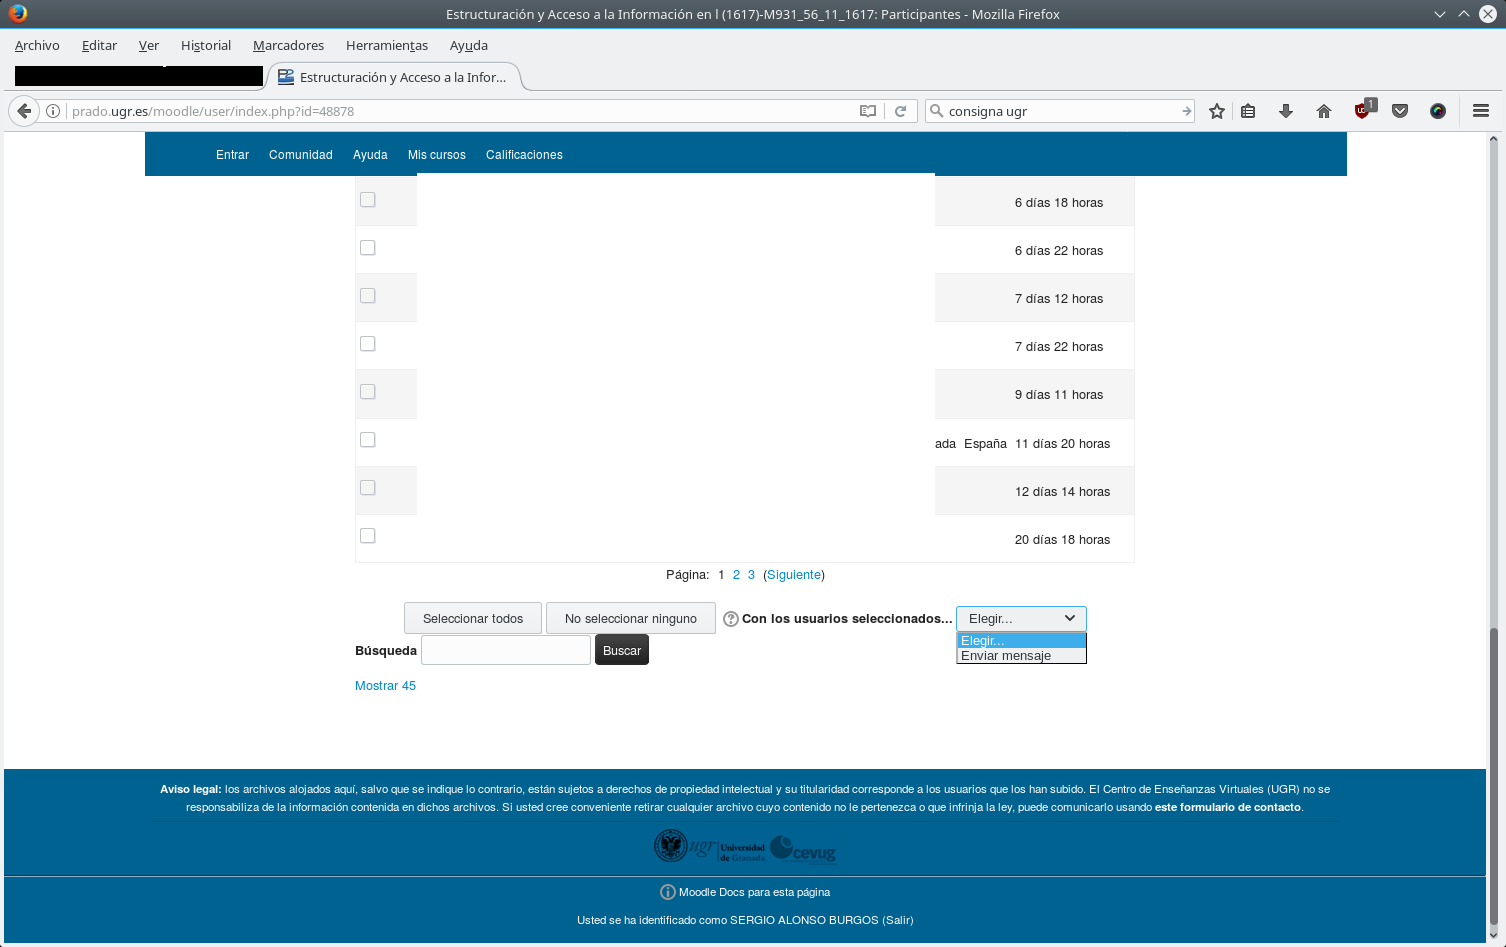
\includegraphics[width=0.8\textwidth]{../screenshots/pantallazoPradoenviarMensaje}
\caption{Vista principal del clon de Prado}
\label{fig:Lista desplegable Enviar Mensaje}
\end{figure}

\begin{figure}[h!]
\centering
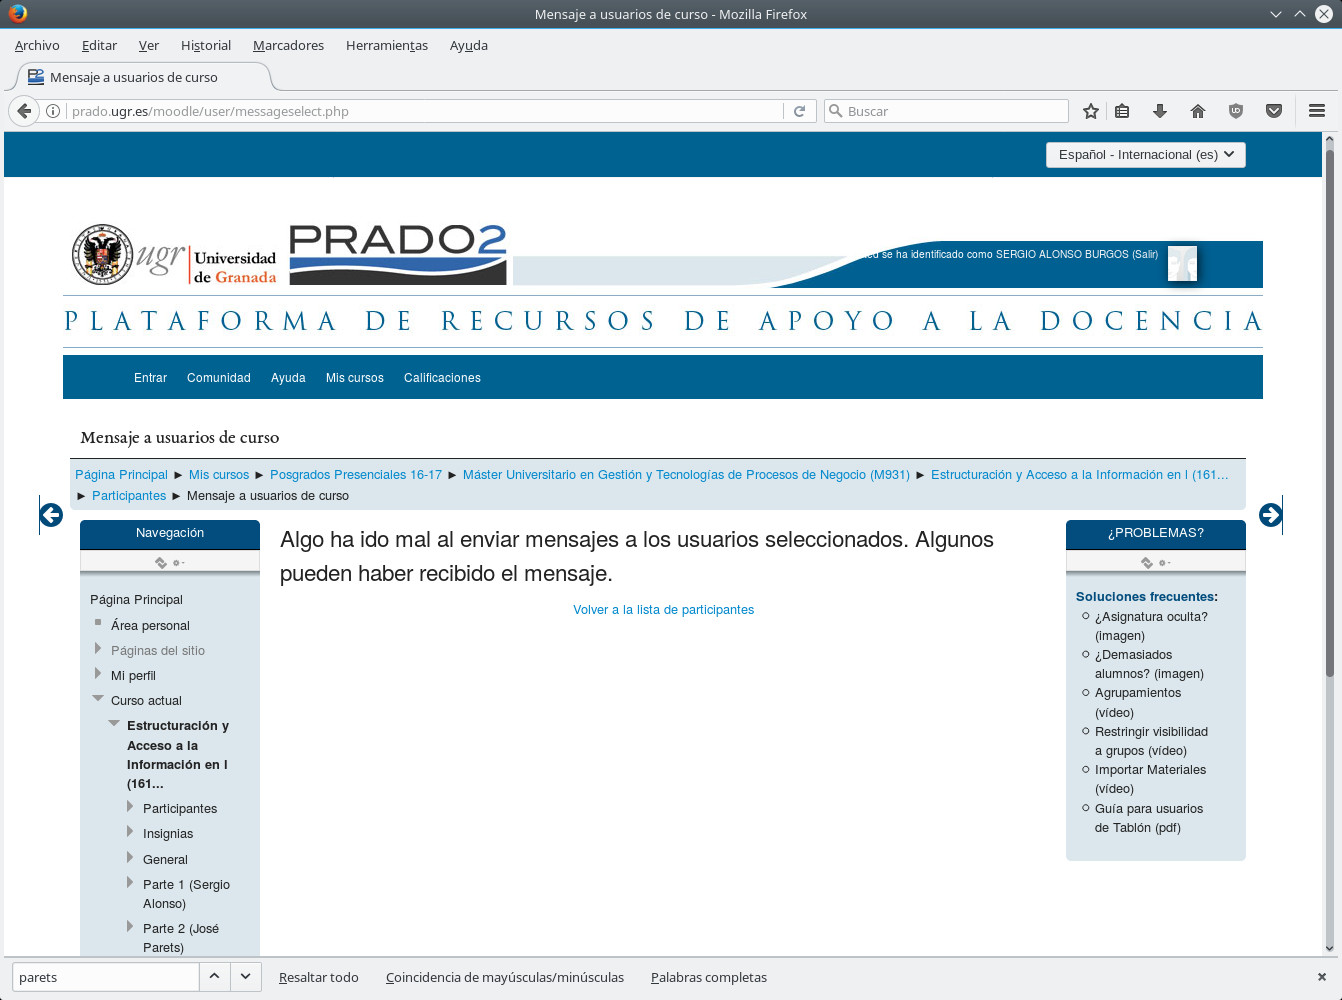
\includegraphics[width=0.8\textwidth]{../screenshots/pantallazoPradoMensaje2}
\caption{Error mostrado al enviar mensaje}
\label{fig:pantallazoPradoMensaje2}
\end{figure}


\item No hay una opción sencilla para crear un listado con los alumnos de cada grupo, opción que puede ser interesante, por ejemplo, para imprimir y llevar un control manual.

\item En la vista de grupos los nombres salen cortados y salen los apellidos de los alumnos pero no aparece el nombre, siendo un problema para alumnos con los mismos apellidos, además no se puede reordenar de ninguna forma.

\item El menú superior de Entrar, Comunidad, Ayuda, Mis cursos no tiene un sentido claro: La opción Entrar aparece siempre aunque la sesión esté iniciada, el menú Comunidad está accesible mas abajo y no tiene una importancia tal y como aparecer en ese menú, el menú Ayuda nos lleva a una pagina externa del CEVUG para abrir un ticket y el menú de cursos lleva a una vista que no es la misma que la de la página principal de Prado2.

\item La búsqueda de cursos suele tarda demasiado en responder.

\item Las novedades del curso y del sitio no parecen tener ninguna utilidad.

\item Aunque se configuren agrupamientos de alumnos, los mismos luego no se pueden utilizar para nada, de hecho no sirven ni para hacer un listado de alumnos por grupo.

\item No se entiende la utilidad del foro privado, quizá esa opción no debería estar, igual sucede con las insignias.

\item El árbol de navegación lateral es confuso y la estructura de bloques no es consistente, además en cada cambio de pagina se vuele a mostrar la vista por defecto, se puede hacer la prueba mostrando el bloque de calendario de la parte derecha haciendo click en cambiar de mes, vemos que se recarga la pagina ocultando de nuevo el bloque. Al entrar en la página aparecen a la izquierda 4 bloques diferenciados: Enlaces, Menú Principal, Navegación y Administración pero al entrar en cualquier opción los dos primeros desaparecen.

\item En los listados no se puede ordenar por rol del usuario, por lo que los distintos profesores de una asignatura aparecen mezclados con los alumnos.

\item Aunque se oculten los bloques laterales con las flechas que hay para tal cometido al recargar la página esos bloques vuelven a aparecer.


\item Si hago colapsar las columnas de navegación laterales (flechas izquierda y derecha), en cuanto pincho en otro enlace me vuelven a aparecer. Tengo que estar colapsándolas todo el rato.

\item Las herramientas de grupos/agrupamientos me han dado algo de trabajo. Creo que ya lo controlo, pero me da la sensación de que podrían ser más fáciles.
\item Si envío un mensaje a un estudiante a través de moodle, no puedo poner un 'Asunto'. Imagino que simplemente le sale en 'Asunto' el nombre de la asignatura, pero me gustaría poder poner algo más específico.
\item Todos los cursos pongo un cuestionario de valoración de la asignatura que los estudiantes pueden responder anónimamente. Moodle preserva el anonimato en las respuestas, pero no en el 'registro de actividad'. Es decir, se puede saber quiénes respondieron al cuestionario e incluso, si uno estuviera muy pendiente de cada actualización de respuestas, quién es responsable de cada respuesta. Creo que cuando una actividad se etiqueta como anónima, el acceso a la misma debería desaparecer del registro de actividad.
\item Al poner una fecha de inicio y fin de una actividad, debería aparecer por defecto el año en que estamos. En una ocasión me ocurrió que la actividad se daba por cerrada un año antes.
\item No sé de quién depende esto pero, por favor, que aparezcan en moodle todos los estudiantes matriculados en la asignatura, y sólo ellos.

\item Es una locura el tema de la matrícula de los estudiantes; me han escrito estudiantes para decirme que a pesar de estar en otro curso y no haberse matriculado nunca en mi asignatura, aparecen y, por tanto, les llegan los mensajes y tienen acceso a la plataforma. Por el contrario, hay muchos estudiantes que tengo que matricular manualmente porque, a pesar de estar en mi grupo, no aparecen!!! 

\item El problema de la adjudicación de grupos de alumnos en el master de educación. Aparecen los alumnos de todas las especialidades en la misma asignatura y todos los profesores pueden subir o borrar recursos de la plataforma, aunque no sean profesores de ese grupo en concreto.



-Las sesiones de usuario (sobre todo cuando se visualiza desde el smartphone) se mantienen de una forma muy rara, ha habido veces que se ha cerrado sin motivo alguno y hay que volver a iniciar sesión. Adicionalmente, se debería habilitar un botón para recordar la sesión.
-La usabilidad deja mucho que desear, la plataforma no es nada intuitiva.
-En general los profesores no saben utilizar la opción de elegir grupo, optando por pasar una hoja en papel y que cada uno se apunte donde quiera.
-No se muestra con claridad los archivos nuevos o novedades en general, de forma que el usuario tiene que estar buscando qué ha visto ya y qué no.
-La plataforma funciona con lentitud y las caídas son muy frecuentes, en ocasiones en horas críticas para la entrega de ejercicios (entre las 22:00 y las 00:00)
-La plataforma en general carece de estilo y orden alguno, las cosas están por medio sin una estructura de calidad.

  Estaba haciendo unas cosas del Departamento y he tenido que acceder a Prado. Entonces he caído en la cuenta de otras dos cosas que no tenía anotadas y para las que no hay opción directa en Prado: poner el horario de teoría y prácticas de la asignatura y poner el horario de tutorías del profesorado implicado (tampoco sale en la parte personal). En general, los datos de la asignatura (incluso objetivos, temario de teoría y temario de prácticas) y los del profesorado que la imparte, brillan por su ausencia. Dos puntos más, y gordos, a favor de SWAD.

  Todas esas cosas las he podido poner en Prado, pero en un archivo en pdf que yo me he creado con la presentación de la asignatura.


\end{enumerate}

\section{Encuesta a los usuarios}

Durante el tiempo que estuvo operativa la encuesta recibimos un total de 617 respuestas, como se puede apreciar en el gráfico la mayor parte de las respuestas se obtuvieron tras las peticiones de participación via e-mail.

    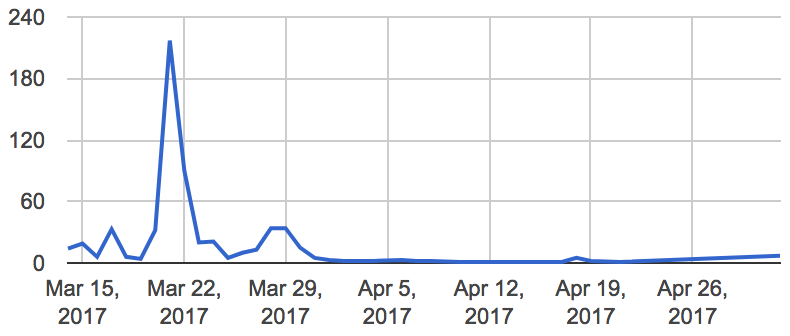
\includegraphics[width=0.8\textwidth]{../charts/00_fecha}
 	

\begin{enumerate}

  \item \textbf{Selección del tipo de usuario} 
  
  La mayor parte de los encuestados han sido alumnos superando el 83\% del ratio, casi un 15\% han sido profesores y el resto otro tipo de usuarios como pueden  ser estudiantes de doctorado y antiguos alumnos.
  
  
	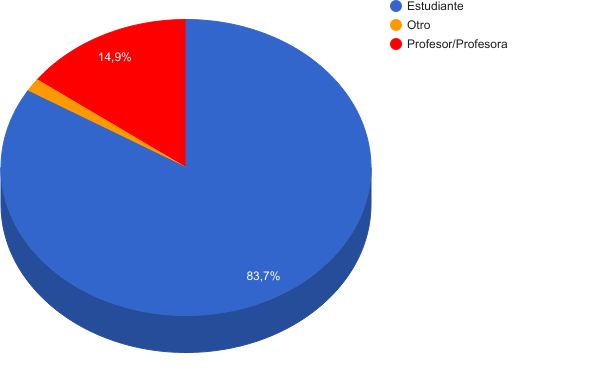
\includegraphics[width=0.8\textwidth]{../charts/01_esusted}
  

  \item \textbf{Selección de la titulación} 
  
  Debido al carácter de este proyecto esperábamos una mayoría de participantes de estudiantes de carreras impartidas en la ETSIIT como pueden ser el Grado de Ingeniería Informática, el Grado de Ingeniería en Tecnologías de Telecomunicación y el Doble Grado en Ingeniería Informática y Matemáticas, pero nos ha sorprendido ver la alta participación de otros estudios como pueden ser Administración y Dirección de Empresas, Medicina y Psicología por nombrar las titulaciones mas representativos de las casi 70 participantes.
  
  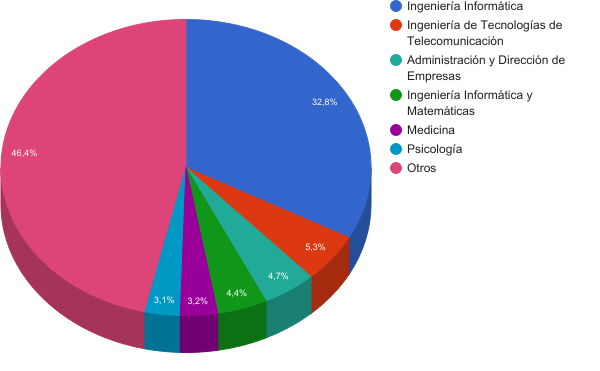
\includegraphics[width=0.8\textwidth]{../charts/02_titulacion}


  \item \textbf{¿Con qué periodicidad accede a Prado2?} 
  
  La mayoría de los usuarios acceden a la plataforma con mucha frecuencia lo que refuerza nuestra opinión de que por un lado se tiene que optimizar la plataforma para que esos accesos sean lo mas breves y satisfactorios posibles, muchos de estos accesos se reducirían si el sistema notificara vía e-mail o a través de un aplicación móvil si hay alguna actividad nueva en mis cursos. De igual manera se reduciría carga en el servidor si se supiera que los documentos subidos por el profesor no han subido cambios y no hubiera que descargarlos de nuevo para comprobarlo manualmente.

  
  
  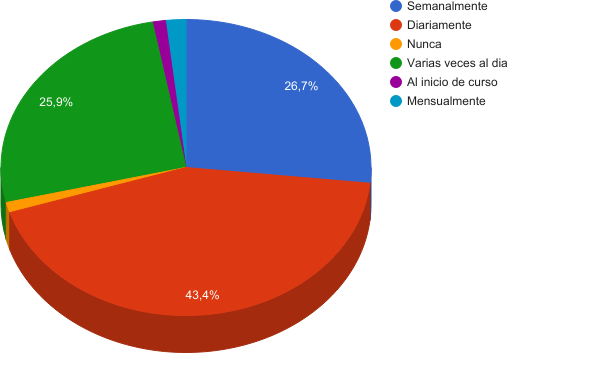
\includegraphics[width=0.8\textwidth]{../charts/03_periodicidad}

  
  \item \textbf{Califique las siguientes opciones según sus necesidades} 

Lo que mas piden los usuarios con diferencia es poder ver las calificaciones en Prado2, eso nos lo han hecho saber tanto en la opción de la encuesta como varios comentarios personales. Por otra parte muchos profesores nos han hecho saber que con el sistema actual tiene que hacer el trabajo por duplicado introduciendo las calificaciones en Prado2 y por otro lado en el sistema de actas de la UGR, cuando sería muchos mas cómodo poder generar en prado algún tipo de fichero CSV que les permitiera entregar las actas.

  
Casi todos los usuarios coinciden en que es vital el acceso desde dispositivos móviles, ya sea mediante una aplicación para smartphone como desde una web con un diseño adaptado a móviles ya que aunque el diseño actual tiene partes que si se adaptan para móviles no es apto para su uso ya que se hace inmanejable.

Los usuarios también creen necesario un sistema de mensajería interna para la comunicación entre profesores y alumnos.

En cambio, las opciones de Insignias, Blogs y Estadísticas no parecen ser vitales y de hecho mucha gente nos ha preguntado que utilidad tienen las Insginias pues no saben para que sirven.

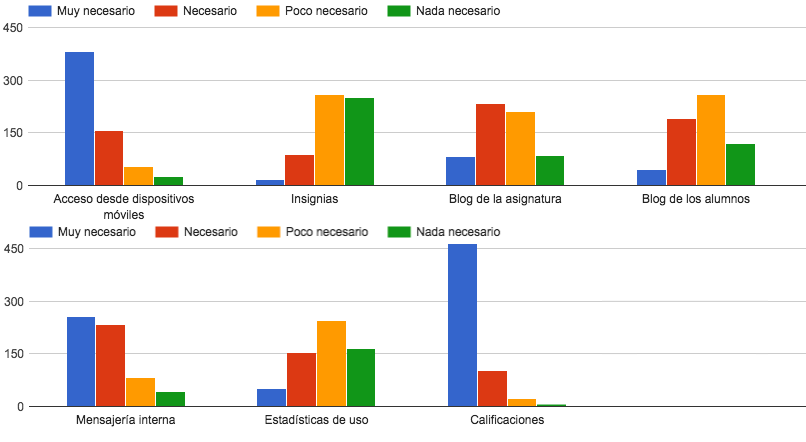
\includegraphics[width=0.8\textwidth]{../charts/04_califique} 

  \item \textbf{Actividades y recursos} 

En cuanto a actividades podemos ver que al igual que en las instalaciones de moodle de otras universidades las opciones mas usadas son las de agregar tareas y archivos, hay que tener en cuenta que hay actividades que básicamente son similares a agregar archivo, como puede ser carpeta, documento, página y libro. 

Aunque moodle tiene actividades que podrían ser muy útiles, como pueden ser los paquetes SCORM e IMS, el desconocimiento y/o la falta de formación hace que la gente ignore para que sirven.

Igual pasa con algunas tareas específicas creadas para la UGR como pueden ser las clases grabadas (GA3), aunque si hay tareas que son necesarias aunque tengan muy poca utilización como pueden ser la selección de grupo de prácticas al inicio del curso y el control de asistencia.


\begin{figure}[H]
\centering
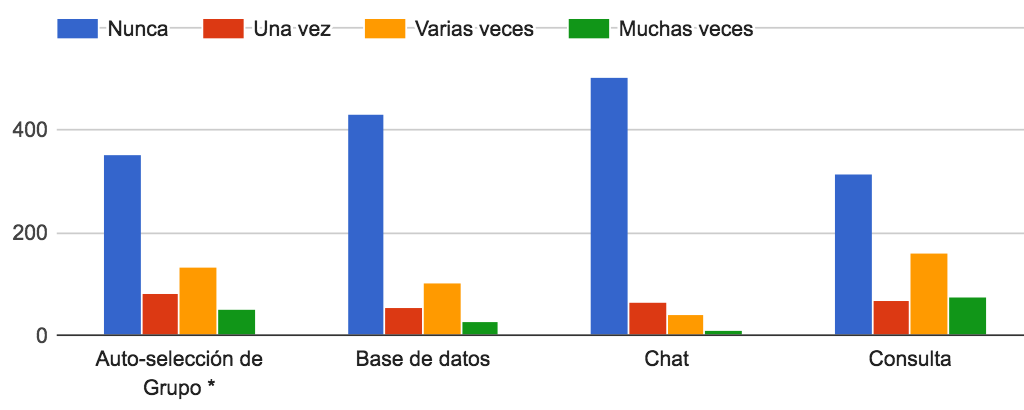
\includegraphics[width=0.8\textwidth]{../charts/05_actividades_01} 
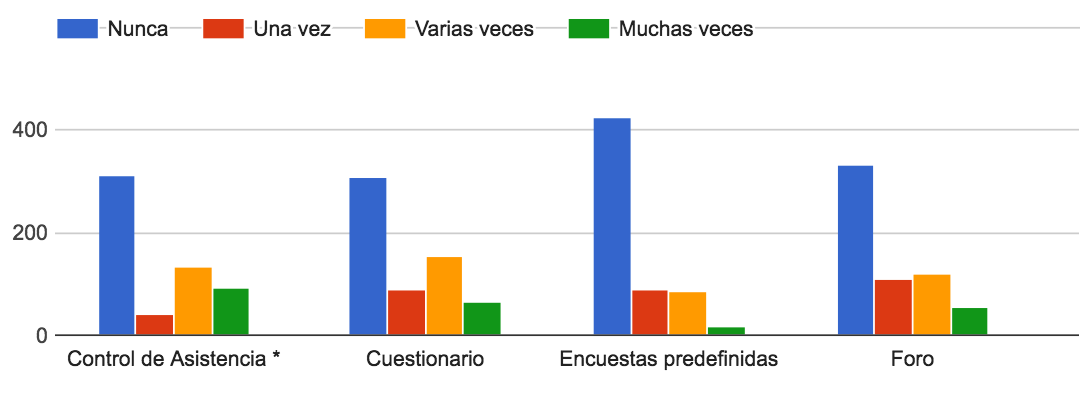
\includegraphics[width=0.8\textwidth]{../charts/05_actividades_02} 
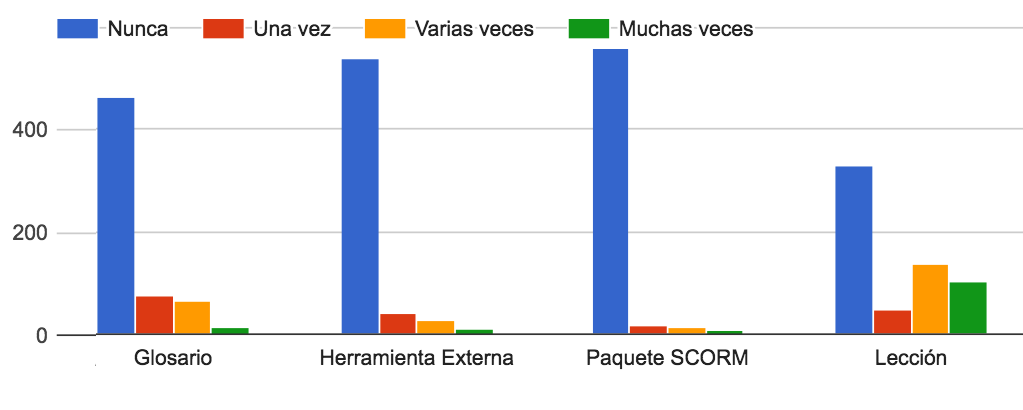
\includegraphics[width=0.8\textwidth]{../charts/05_actividades_03} 
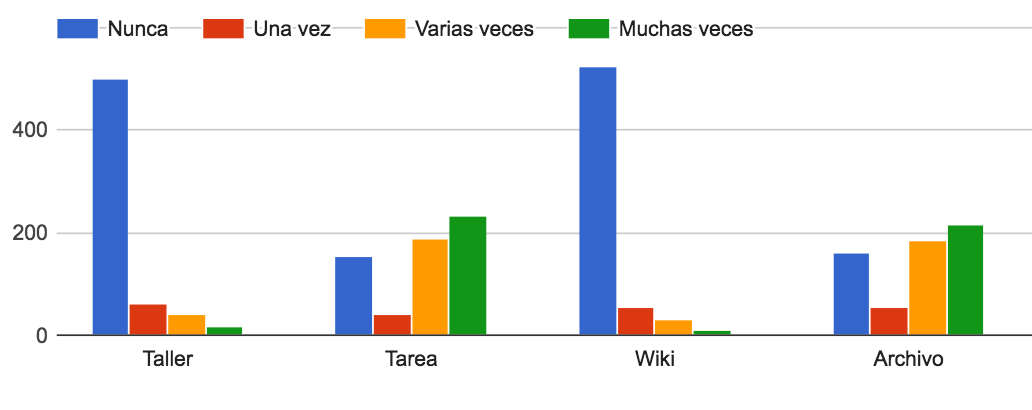
\includegraphics[width=0.8\textwidth]{../charts/05_actividades_04} 
\end{figure}
\begin{figure}[H]
\centering
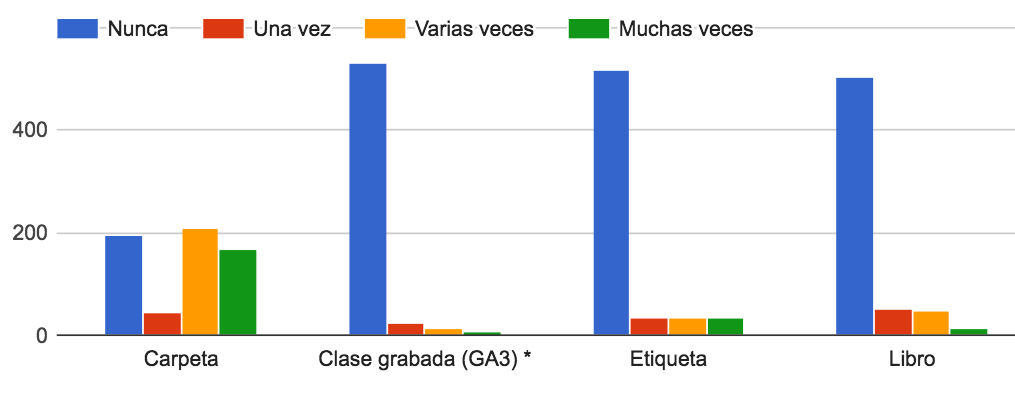
\includegraphics[width=0.8\textwidth]{../charts/05_actividades_05} 
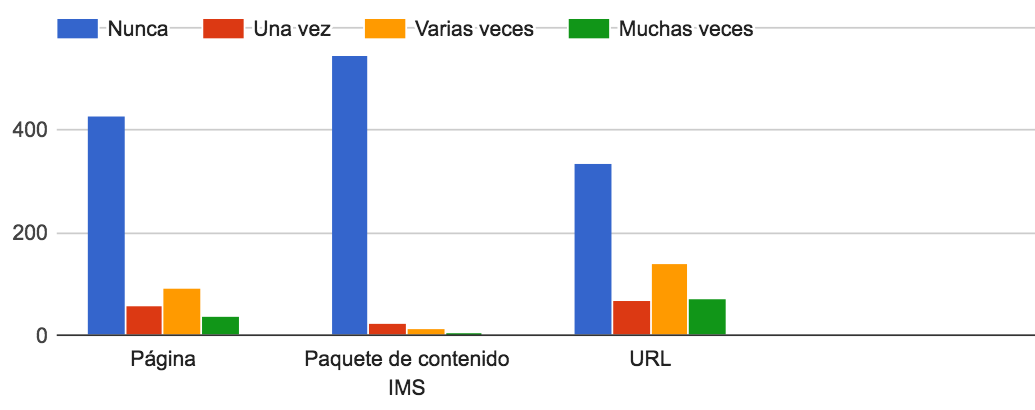
\includegraphics[width=0.8\textwidth]{../charts/05_actividades_06} 

\end{figure}

  \item \textbf{¿Cómo calificaría Prado2?}
  
  
A la hora de calificar prado han la mayoría de los usuarios han otorgado aprobado lo cual es una buena señal, aunque se piense que hay un descontento generalizado la gente entiende que una plataforma puede tener problemas y simplemente espera que se solucionen. Aun con el aprobado general, los usuarios si que encuentran en gran medida muy deficiente la usabilidad de la plataforma. En cambio el sentimiento general es el de que la plataforma es segura.

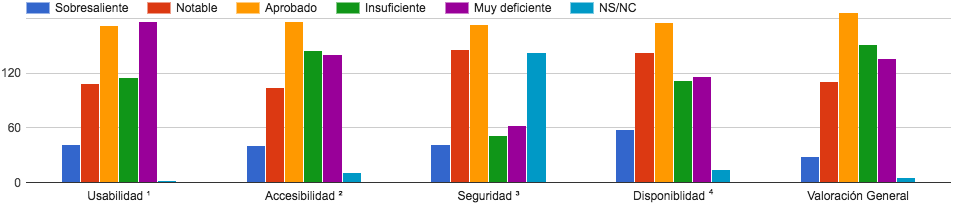
\includegraphics[width=0.8\textwidth]{../charts/06_calificaria}


  \item \textbf{¿Con cúales de las siguientes plataformas de la UGR ha trabajado?} 

Aquí hay tres ganadores claves, y son evidentemente las plataformas que mas se han usado en todo el ámbito UGR como pueden ser el Tablon de Docencia, SWAD y el propio Prado2, luego encontramos plataformas usadas solo en la ETSIIT como pueden ser Tutor y DECSAI y algunos otros como el antiguo moodle del CEVUG y Ágora que es otra instalación de moodle utilizada en la facultad de Psicología.

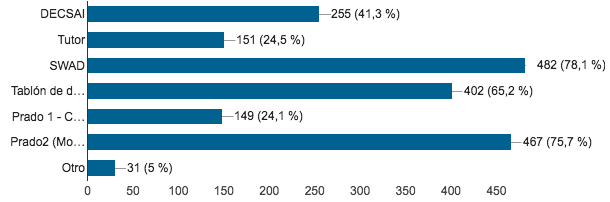
\includegraphics[width=0.8\textwidth]{../charts/07_plataformastrabajado}

  \item \textbf{De las siguientes plataformas de la UGR ¿Cuál prefiere?} 

A la hora de establecer la plataforma favorita está clara la prevalencia de SWAD ya que es una plataforma potente y con muchos años de uso aunque Prado2 también tiene una buena acogida y mas teniendo en cuenta la sensación de descontento generalizado que percibíamos antes de comenzar este proyecto, esto quiere decir que tampoco se va por mal camino con la plataforma actual. Curioso cuanto menos que el Tablón de Docencia, una arcaica plataforma utilizada en la UGR sigue teniendo sus partidarios pero como ya hemos comentado anteriormente una de las cosas con las que más cuesta lidiar en cuanto a la usabilidad es la resistencia de los usuarios al cambio, aunque este sea a mejor.

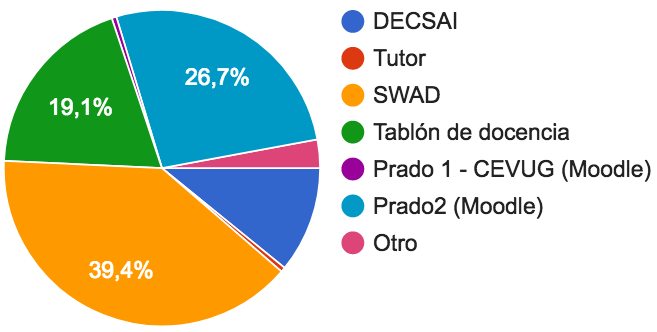
\includegraphics[width=0.8\textwidth]{../charts/08_plataformas_prefiere} 

  \item \textbf{¿Ha encontrado algún error que debería ser subsanado en Prado2?} 

Esta pregunta al ser de entrada libre se adjuntará en el listado en bruto de respuestas   

  \item \textbf{Indique cuál es la funcionalidad que más le gusta de Prado2} 

Esta pregunta al ser de entrada libre se adjuntará en el listado en bruto de respuestas

  \item \textbf{Comentarios adicionales} 
  
Esta pregunta al ser de entrada libre se adjuntará en el anexo VI
  
\end{enumerate}


\section{Análisis de registros propios de la plataforma}

Tras analizar los registros proporcionados por el CEVUG de los años 2015 y 2016 vemos que los resultados de la encuesta cuadran con los mismos.

No hemos analizado la muestra que nos proporcionaron de 2014 ya que fue en el curso 2015-2016 como se puede apreciar en la figura \ref{fig:distintonumerousuarios_2015}.

Lo primero a destacar son el notable incremento de peticiones del año 2015 al año 2016 que se puede apreciar en la tabla de la figura \ref{table:sumarioregistros}.

\begin{table}[H]
\centering
\begin{tabular}{|l|r|r|}
\hline
\textbf{Año}        & \textbf{2015}	& \textbf{2016} 		\\ \hline
Número de registros & 3.119.094     	& 20.243.312			\\ \hline
Usuarios únicos     & 19.448        & 51.283				\\ \hline
IPs distintas       & 115.349       & 370.580			\\ \hline
Cursos              & 1.266         & 8.414				\\ \hline
Módulos             & 32            & 32					\\ \hline
\end{tabular}
\caption{Sumario de los registros de los años 2015 y 2016}
\label{table:sumarioregistros}
\end{table}

En las figuras de la \ref{fig:actividadtotal_2015} a la \ref{fig:frecuenciausuarios_2016} podemos ver como el grueso de la actividad se lo llevan unos pocos usuarios, es decir, la inmensa mayoría interactúa muy poco con la plataforma. Presuponemos que este grueso de actividad pertenece tanto a los administradores como a un reducido círculo de profesores, hay que tener en cuenta que los logs registran cada click en alguna sección de Prado.

\begin{figure}[H]
\centering
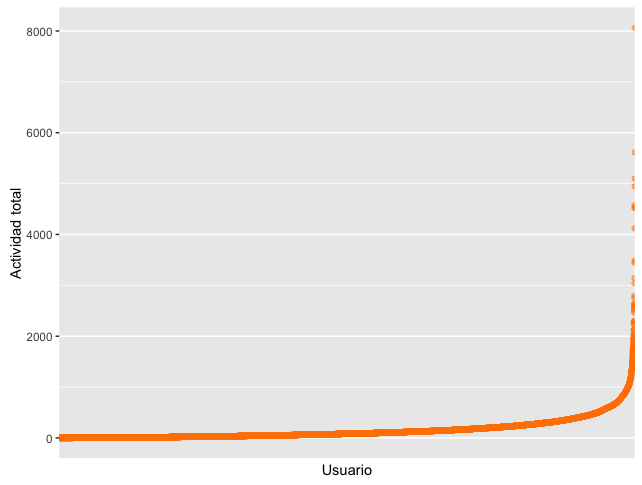
\includegraphics[width=0.9\textwidth]{../r/actividadtotal_2015}
\caption{Actividad total en 2015}
\label{fig:actividadtotal_2015}
\end{figure}

\begin{figure}[H]
\centering
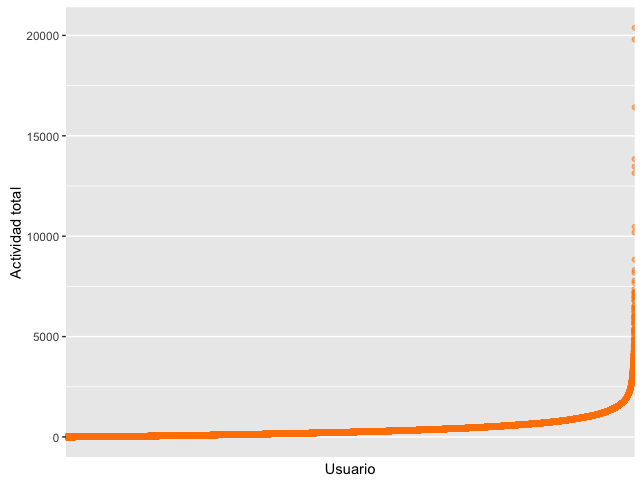
\includegraphics[width=0.9\textwidth]{../r/actividadtotal_2016}
\caption{Actividad total en 2016}
\label{fig:actividadtotal_2016}
\end{figure}

\begin{figure}[H]
\centering
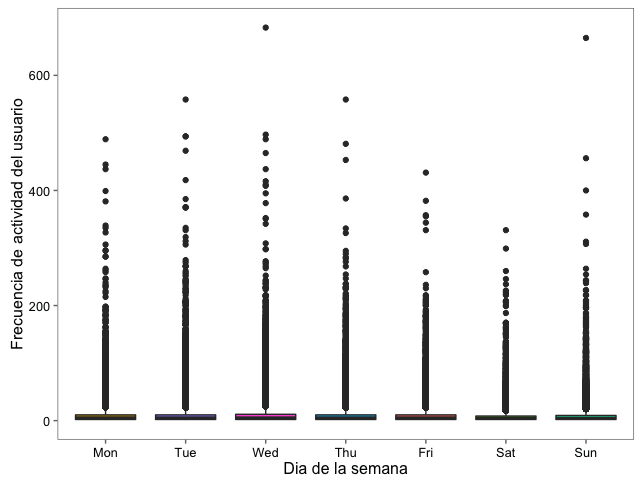
\includegraphics[width=0.9\textwidth]{../r/frecuenciaactividadusuario_2015}
\caption{Frecuencia de actividad de los usuarios en 2015}
\label{fig:frecuenciaactividadusuario_2015}
\end{figure}

\begin{figure}[H]
\centering
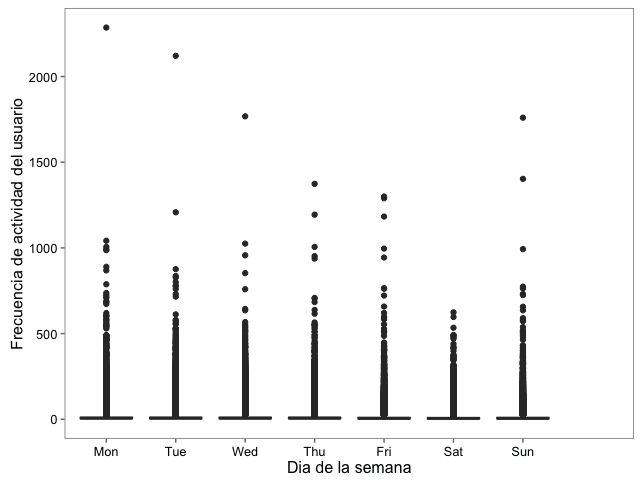
\includegraphics[width=0.9\textwidth]{../r/frecuenciaactividadusuario_2016}
\caption{Frecuencia de actividad de los usuarios en 2016}
\label{fig:frecuenciaactividadusuario_2016}
\end{figure}


\begin{figure}[H]
\centering
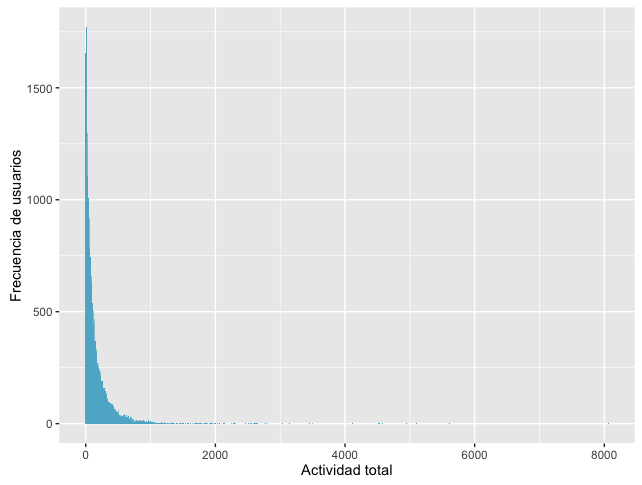
\includegraphics[width=0.9\textwidth]{../r/frecuenciausuarios_2015}
\caption{Frecuencia de usuarios en 2015}
\label{fig:frecuenciausuarios_2015}
\end{figure}


\begin{figure}[H]
\centering
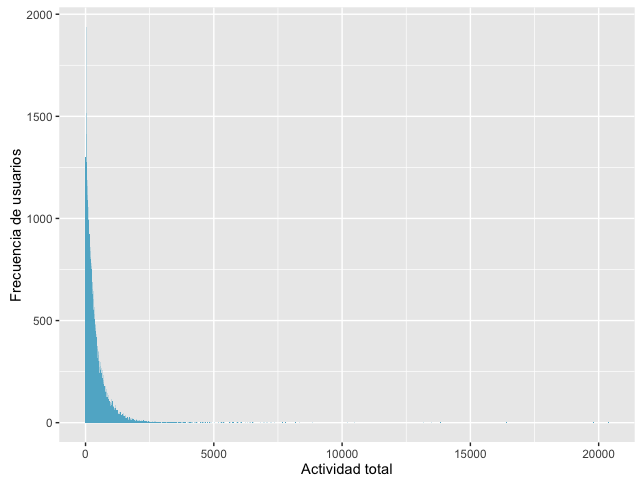
\includegraphics[width=0.9\textwidth]{../r/frecuenciausuarios_2016}
\caption{Frecuencia de usuarios en 2016}
\label{fig:frecuenciausuarios_2016}
\end{figure}

También vemos en las figuras \ref{fig:distintonumerousuarios_2015} y \ref{fig:distintonumerousuarios_2016} como los usuarios comenzaron a hacer uso de la plataforma en Septiembre de 2015 que es cuando oficialmente se comenzó a utilizar Prado.



\begin{figure}[H]
\centering
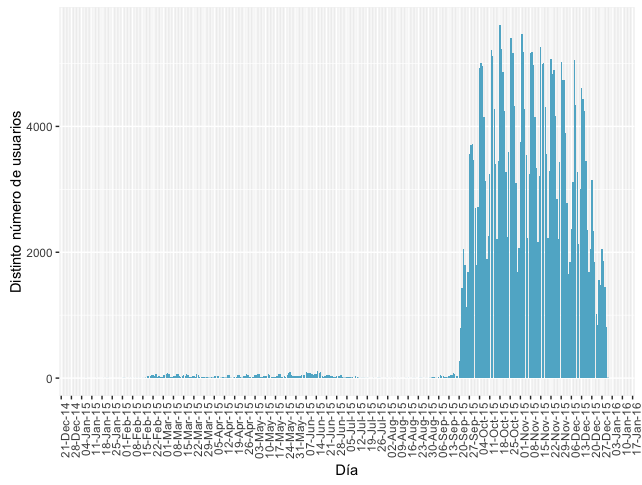
\includegraphics[width=0.9\textwidth]{../r/distintonumerousuarios_2015}
\caption{Interacciones de usuarios únicos en 2015}
\label{fig:distintonumerousuarios_2015}
\end{figure}

\begin{figure}[H]
\centering
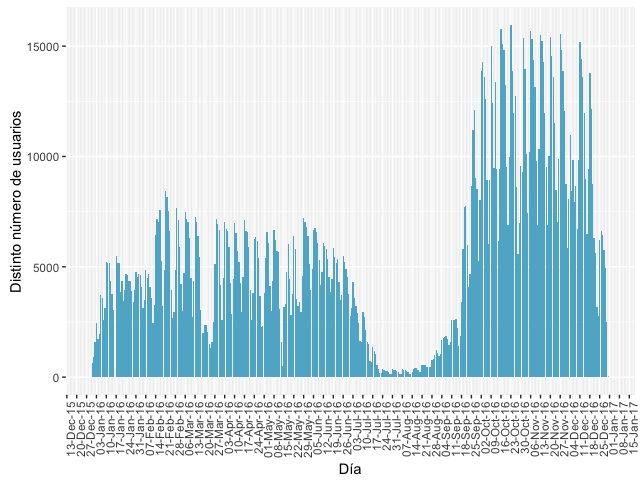
\includegraphics[width=0.9\textwidth]{../r/distintonumerousuarios_2016}
\caption{Interacciones de usuarios únicos en 2016}
\label{fig:distintonumerousuarios_2016}
\end{figure}


En las figuras \ref{fig:frecuenciaactividaddiaria_2015} y \ref{fig:frecuenciaactividaddiaria_2016} se percibe como la mayoría de los usuarios utilizan la plataforma en las horas lectivas, descenciendo la utilización como es evidente los fines de semana, también nos sirve para ver como la madrugada es la hora ideal para realizar cambios en la plataforma pues el a esas horas casi no hay usuarios usando Prado.

\begin{figure}[H]
\centering
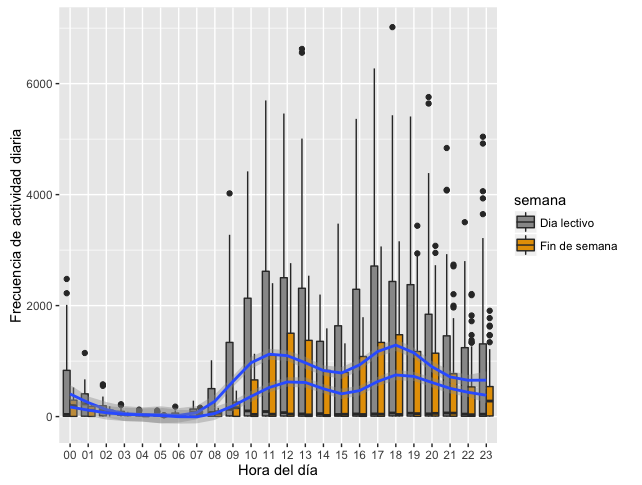
\includegraphics[width=0.9\textwidth]{../r/frecuenciaactividaddiaria_2015}
\caption{Frecuencia de actividad diaria en 2015}
\label{fig:frecuenciaactividaddiaria_2015}
\end{figure}

\begin{figure}[H]
\centering
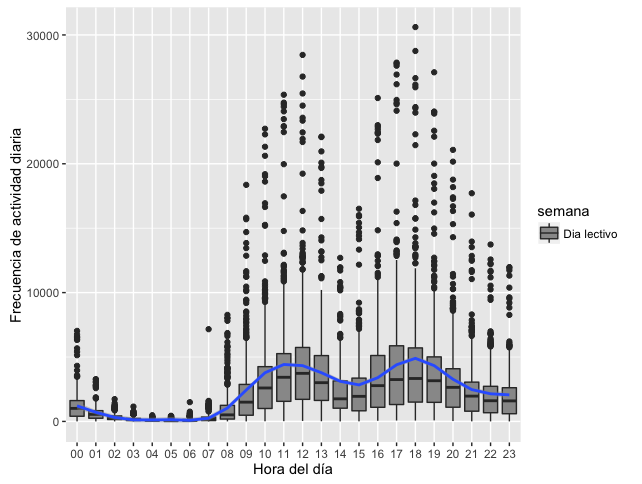
\includegraphics[width=0.9\textwidth]{../r/frecuenciaactividaddiaria_2016}
\caption{Frecuencia de actividad diaria en 2016}
\label{fig:frecuenciaactividaddiaria_2016}
\end{figure}


En cuanto a las actividades podemos ver en las figuras \ref{fig:usoactividades_2015} y \ref{fig:usoactividades_2016} así como en la tabla \ref{table:usoactividades_2015} que tal y como concluimos en la encuesta la gran mayoría de las actividades disponibles en moodle no tienen apenas uso. Hay que destacar que la actividad 'course' se refiere a cada vez que un usuario ve contenido de un curso acaparando la mitad de las interacciones, la actividad 'user' se crea cada vez que se ve el perfil de un usuario o profesor y la actividad 'assign' es para uso interno de moodle. Exceptuando estos tres casos vemos como las mas usados los cuestionarios y los archivos.

\begin{figure}[H]
\centering
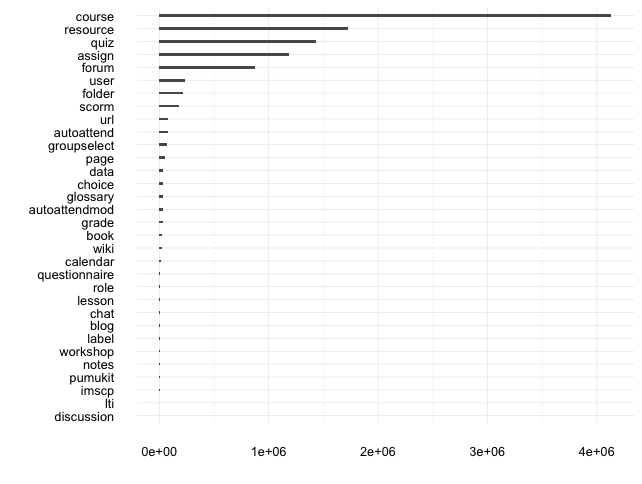
\includegraphics[width=0.9\textwidth]{../r/usoactividades_2015}
\caption{Uso de actividades en 2015}
\label{fig:usoactividades_2015}
\end{figure}

\begin{figure}[H]
\centering
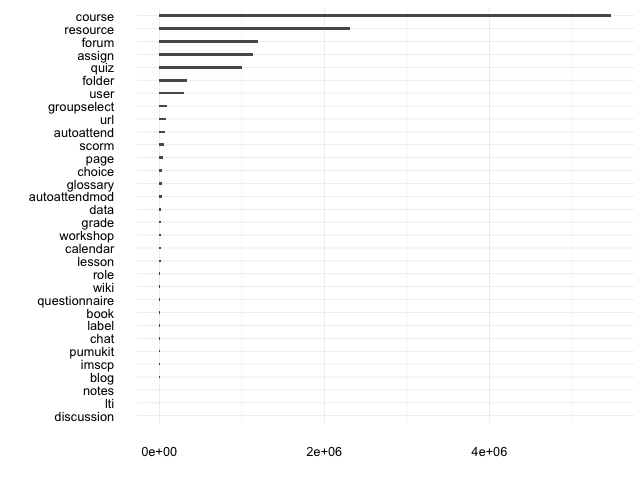
\includegraphics[width=0.9\textwidth]{../r/usoactividades_2016}
\caption{Uso de actividades en 2016}
\label{fig:usoactividades_2016}
\end{figure}

\begin{table}[H]
\centering
\begin{tabular}{|l|r|r|}
\hline
\textbf{Módulo} & \textbf{2015} & \textbf{2016} \\ \hline
course          & 1204043       & 8631749       \\ \hline
quiz            & 480975        & 1967505       \\ \hline
resource        & 464898        & 3680181       \\ \hline
assign          & 381096        & 1985887       \\ \hline
forum           & 233528        & 1905834       \\ \hline
user            & 81118         & 473303        \\ \hline
folder          & 65733         & 499643        \\ \hline
scorm           & 33459         & 205890        \\ \hline
url             & 25720         & 139415        \\ \hline
autoattend      & 25530         & 112115        \\ \hline
groupselect     & 25518         & 132941        \\ \hline
page            & 22382         & 79816         \\ \hline
choice          & 11514         & 58419         \\ \hline
autoattendmod   & 11020         & 47220         \\ \hline
glossary        & 9244          & 50541         \\ \hline
lesson          & 6702          & 14140         \\ \hline
wiki            & 6040          & 26199         \\ \hline
calendar        & 4988          & 23273         \\ \hline
questionnaire   & 4961          & 13241         \\ \hline
data            & 4525          & 51868         \\ \hline
book            & 4485          & 31140         \\ \hline
grade           & 2809          & 46357         \\ \hline
role            & 2306          & 16770         \\ \hline
blog            & 1665          & 4616          \\ \hline
chat            & 1351          & 7267          \\ \hline
label           & 1282          & 7014          \\ \hline
notes           & 1174          & 3362          \\ \hline
imscp           & 396           & 2789          \\ \hline
pumukit         & 305           & 4717          \\ \hline
discussion      & 118           & 344           \\ \hline
workshop        & 117           & 18395         \\ \hline
lti             & 92            & 1357          \\ \hline
\end{tabular}
\caption{Tabla detallada del uso de actividades en 2015 y 2016}
\label{table:usoactividades_2015}
\end{table}


\section{Análisis de usabilidad de la plataforma}

Analizamos la plataforma como un usuario normal para ver con que problemas se podía encontrar a la hora de usar Prado. Nos hemos centrado en los problemas de usabilidad con fácil solución y que harían la experiencia de usuario mucho más placentera.

\bigskip
En nuestro análisis hemos encontrado los siguientes problemas:

\begin{itemize}

\item Aparece la información para iniciar sesión en la cabecera y en el pié de la página, esto es redundante, debería aparecer solo en la cabecera.
\item El selector de idioma ocupa una gran parte de la pantalla siendo un elemento de uso poco común. De hecho como veremos más adelante la traducción al inglés brilla por su ausencia, lo ideal en estos casos es colocar los enlaces para cambiar el idioma en el pié de página. Hay que tener en cuenta que la plataforma detecta el idioma del navegador para seleccionar Español o Inglés. Además debería poner 'Castellano' en lugar de 'Español - Internacional'.
\item El título 'PLATAFORMA DE RECURSOS DE APOYO A LA DOCENCIA' no debería aparecer como una imagen, ya que además de no estar traducida hace que no todos los dispositivos la muestren bien al ser una imagen demasiado ancha.
\item La ventana de login muestra una imagen con la ruta https hacia el proveedor de identidad del CSIRC, un poco mas abajo nos encontramos un botón con la misma ruta pero con http. El IDP automáticamente redirige a https, este botón debería ocultarse. El acceso para administradores también debería ocultarse.
\item Debajo del banner de título aparece un menú con fondo azul en el que siempre aparece la opción 'Entrar' aunque ya hayamos iniciado la sesión en la plataforma.
\item La opción 'Comunidad' no tiene un uso tan importante como para aparecer ahí, quizá debería estar como un enlace en el pie. Además, podemos acceder al mismo desde el panel lateral.
\item La opción 'Ayuda' lleva a una página externa del CEVUG para solicitar asistencia, al tener un diseño distinto debería abrirse en una ventana nueva.
\item Con la sesión iniciada se muestran los cursos del alumno, pero al haber cursos con el mismo nombre hay que ir probando uno a uno con lo cual esta opción tampoco tiene utilidad.
\item Si se está dentro de un curso también vemos la opción 'Calificaciones', esta opción se puede ver desde el panel lateral y teniendo en cuenta que la mayoría de los profesores no ponen las calificaciones en prado quizá esta opción debería ocultarse.
\item En resumidas cuentas, este menú superior se podría ocultar sin ningún tipo de problema, ganando muchísimo espacio en la pantalla.
\item El banner central de información acapara toda la atención obligando al usuario a desplazarse para ver la información de los cursos que quiere ver. Dicho banner no muestra información útil con lo que quizá merecería quitarlo o por lo menos darle la opción a los usuarios de ocultarlo.
\item Aunque se permite ocultar los paneles laterales al recargar la página se vuelven a mostrar, debería memorizarse el estado seleccionado.
\item Al desplegar las secciones de cada panel lateral ocurre lo mismo que al ocultarlos, no se recuerda cual se tenía abierto. Esto resulta particularmente molesto al hacer uso del calendario en el panel derecho, pues al cambiar de mes se recarga la página ocultando la sección.
\item El panel de la izquierda no sigue un orden lógico, según se va navegando por la página tiene entre 2 y 4 secciones principales aunque contenga la misma información. Pasa lo mismo en el derecho al entrar en una asignatura.
\item El panel derecho muestra una sección de 'Problemas' con información para los profesores que los alumnos no deberían de ver.
\item Al ver nuestro perfil no debería mostrarse la opción 'Personalizar esta página' ya que esto es lo que se usa para editar los cursos. Esto lleva a confusión al usuario pues piensa que esta opción es para editar su perfil y no es así.
\item Las insignias deberían ocultarse pues no se están utilizando.
\item Hay diversas vistas diferentes de 'Mis cursos', lo cual es bastante confuso.
\item Una vez dentro de un curso el foro de novedades se debería ocultar por defecto a no ser que el profesor lo active.
\item En la vista principal de la asignatura, para ver los archivos hay que desplegar primero las diferentes opciones, quizá sería mejor mostrar un árbol para poder desplegarlo todo de una vez en lugar de uno en uno.
\item Al entregar una tarea muchas veces se olvida de enviar para calificación, lo ideal sería que por defecto al crear una tarea sea el envío automático para calificación.
\item No se puede ver si han habido cambios en los archivos subidos por el profesor, ni la fecha de subida ni ninguna información. De hecho, el nombre del archivo no tiene por qué coincidir con el texto que aparece en Prado, aumentando la confusión.
\item No se pueden descargar todos los archivos de una asignatura de golpe, hay que ir uno a uno.
\item Cuando un profesor está en modo edición puede agregar archivos de forma sencilla arrastrándolos sobre la ventana de cursos, pero la web no lo explica. En la plantilla por defecto de moodle si que sale una notificación informando de esta funcionalidad. Esto se debería mostrar ya que facilita mucho la tarea de subir archivos a la plataforma.
\item Cuando un profesor va a agregar una actividad el menú que sale es enorme, quizá se debería mostrar los mas utilizados, dejar el resto ocultos y permitir mostrarlo en una vista avanzada.
\item La vista de 'Todos los cursos' se debería ocultar, pues es imposible utilizar un desplegable con mas de 1000 opciones.
\item La vista 'Novedades del sitio' no muestra nada y al seleccionarla cambia de posición en el panel lateral, lo ideal sería ocultarla.
\item Se muestran varias asignaturas iguales, esto es confuso. Aunque internamente se creen para facilitar la administración lo ideal sería agruparlas en la misma vista para los alumnos.
\item El sistema de mensajería contiene un desplegable con la opción 'Enviar mensaje', para una sola opción sería mas sencillo un botón.

\end{itemize}

\section{Análisis de accesibilidad de la plataforma}

Los resultados de los análisis automáticos de accesibilidad de la página principal de Prado (ver figuras \ref{fig:tawdis}, \ref{fig:tenon} y \ref{fig:htmlcodesniffer}) indican que la plataforma tiene algunos puntos que corregir para cumplir con el estándar AA de accesibilidad. No se ha podido analizar de forma automática las páginas internas pues dichas herramientas no pueden acceder a la Plataforma porque hay que autentificarse. El resultado de dicho análisis automático es positivo pues la gran mayoría son pequeños detalles como asignación de etiquetas \texttt{alt}\footnote{Las etiquetas 'alt' se usan en las imágenes como “alternate text”, es decir, un texto que describe la imagen.} en imágenes. 

\bigskip
El test TAW nos indica que los colores de la plataforma pueden llegar a generar confusión y que sería adecuado un esquema de colores que permita distinguir de forma mas fácil la información importante así como las secciones principales.

\begin{figure}[H]
\centering
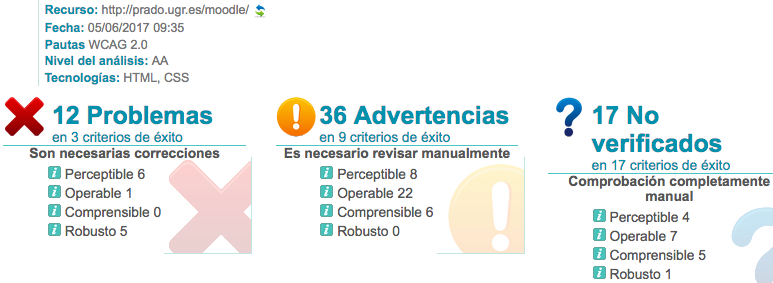
\includegraphics[width=0.9\textwidth]{../screenshots/tawdis}
\caption{Resultados de usabilidad con TAW}
\label{fig:tawdis}
\end{figure}

\begin{figure}[H]
\centering
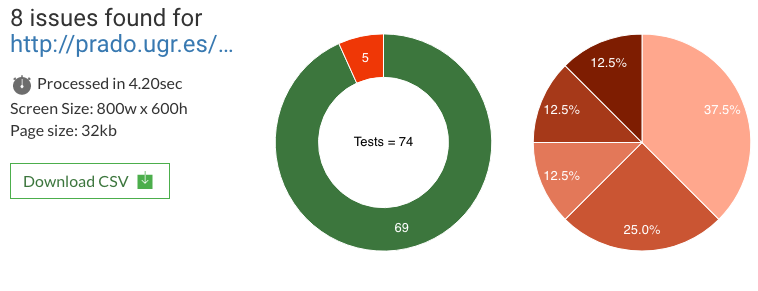
\includegraphics[width=0.8\textwidth]{../screenshots/tenon}
\caption{esultados de usabilidad con tenion.io}
\label{fig:tenon}
\end{figure}

\begin{figure}[H]
\centering
\includegraphics[width=0.6\textwidth]{../screenshots/htmlcodesniffer}
\caption{esultados de usabilidad con HTML CodeSniffer}
\label{fig:htmlcodesniffer}
\end{figure}


\bigskip
Aunque la plantilla utilizada es responsive\footnote{El diseño web responsive o adaptativo es una técnica de diseño web que busca la correcta visualización de una misma página en distintos dispositivos, desde ordenadores de escritorio a tablets y móviles}, los cambios realizados en la misma hacen que sea bastante incómoda de utilizar. Por un lado la vista principal debería mostrar mis cursos sin obligar a desplazarnos hacia abajo para obviar el mensaje de bienvenida. Al acceder a información como pueden ser calificaciones o entregas al no estar correctamente adaptado hay desplazarse horizontalmente y se pierde la noción de donde se está exactamente.

\bigskip
En la figura \ref{fig:capturamovil2} podemos ver como la ventana de inicio de sesión muestra una imagen que no está adaptada, con un botón mas abajo que realiza la misma función dando lugar a confusión, el acceso para personal técnico tampoco debería visualizarse y en la cabecera vemos como hay mucho espacio desperdiciado sin mostrar nada.

\bigskip
La plantilla tiene un menú 'hamburguesa' debajo de la imagen de perfil pero el ajuste realizado a la misma hace que se muestre parcialmente impidiendo su correcta utilización.


\begin{figure}[H]
\centering
\includegraphics[width=0.5\textwidth]{../screenshots/capturamovil2}
\caption{Captura desde un teléfono móvil}
\label{fig:capturamovil2}
\end{figure}

\bigskip
La plataforma moodle está disponible en más de 100 idiomas pero en Prado se ha optado por habilitar castellano e inglés. El problema es que gran parte del contenido añadido a la plantilla, la ayuda y la información de los cursos se ha introducido de forma forzada en castellano con lo que el uso en inglés de la plataforma es prácticamente imposible. Varios alumnos de intercambio nos han hecho llegar sus quejas a la hora de manejarse en la plataforma, ya que no entienden que seleccionando la opción de idioma inglés la mayor parte de la interfaz y el contenido aparezca en castellano, creándoles confusión ya que muchos desconocen el castellano.

\bigskip
Si un usuario selecciona el idioma inglés, al ir a la página del IDP del CSIRC para iniciar sesión no se respetará la selección del usuario sino que se obtendrá el idioma del navegador. Esto tendría una solución bastante sencilla pues bastaría pasarle a la url el parámetro \texttt{\&language=<codigo\_iso>} en la llamada al proveedor de identidad.


\section{Análisis de seguridad}

Lo primero que nos llama la atención al realizar la auditoría de seguridad es que la página funciona sobre http, probamos a cargar la página con https y vemos que la página tiene instalado un certificado válido. El motivo de no forzar el protocolo https quizá sea por incompatibilidades de la plantilla, ya que hemos leíd que han arreglado problemas relativos a esto\cite{art_11}. 

\bigskip
Miramos el código fuente de la página y vemos que se están enlazando de manera absoluta hacia http los archivos CSS, esto es lo que hace que la página no se vea correctamente al acceder por https ya que el navegador bloquea las conexiones no https por seguridad. Esto es algo que se resolvería de forma bastante sencilla y evitaría el problema de secuestro se sesión.

\bigskip
Una vez lanzado el programa ettercap le pedimos al tutor que se conectara a Prado y a los pocos segundos obtuvimos el resultado que se puede ver en la figura \ref{fig:ettercap}, en unos pocos segundos y aun estando dentro de una red wifi con cifrado WPA2 pudimos realizar el ataque de ARP Spoofing sin ningún problema. Finalmente obtuvimos las variables de sesión \textbf{MOODLEID1\_}, \textbf{SimpleSAMLSessionID-sp} y \textbf{SimpleSAMLAuthToken}, las cuales copiamos en nuestro navegador con un editor de cookies y de inmediato podíamos navegar suplantando la identidad del tutor.

\bigskip 
Hay que tener en cuenta que para iniciar sesión se utiliza el IDP del CSIRC, que si funciona a través de https por lo que en ningún momento podríamos capturar la contraseña del usuario como si se podría hacer si la página de login funcionara a través de http.

\bigskip
También es un pequeño problema de seguridad el permitir acceder a ficheros README, CHANGELOG y demás, pues esto permite a un posible atacante conocer la versión que se está ejecutando y realizar un ataque utilizando vulnerabilidades conocidas. Si la plataforma se mantuviera constantemente actualizada esto no sería un problema, pero si se va congelar en una versión antigua y sin soporte lo mejor es 'fortificar' la instalación para evitar males mayores.

\begin{figure}[H]
\centering
\includegraphics[width=1.0\textwidth]{../screenshots/ettercap}
\caption{Resultados del ataque mediante ettercap}
\label{fig:ettercap}
\end{figure}



\section{Análisis de disponibilidad}

Como ya hemos indicado anteriormente el 30 de enero de 2017 comenzamos a monitorizar la disponibilidad de Prado2 con la herramienta StatusCake. Como podemos ver en los periodos de disponibilidad de la figura \ref{fig:statuscake1} es una web que realmente goza de una buena disponibilidad por periodos de hasta incluso 40 días. Aunque podemos ver algunos tramos en los que la página no está accesible, estos periodos suelen ser de una duración razonable y a unas horas en las que no se espera que haya demasiados usuarios utilizando la plataforma.

\begin{figure}[h!]
\centering
\includegraphics[width=0.8\textwidth]{../screenshots/statuscake1}
\caption{Disponibilidad medida por StatusCake}
\label{fig:statuscake1}
\end{figure}

\bigskip
Pero vemos como el 13 de marzo de 2017 hubo algún tipo de problema que se tardó bastante en solucionar y que mantuvo la plataforma sin acceso mostrando un mensaje (ver figura \ref{fig:pradocaido}) que tampoco daba a los usuarios demasiada información del problema. El mayor problema de esta caída fue el desconocimiento de los usuarios de qué estaba pasando.

\begin{figure}[h!]
\centering
\includegraphics[width=0.8\textwidth]{../images/pradocaido}
\caption{Mensaje de error mostrado por Prado2}
\label{fig:pradocaido}
\end{figure}

\bigskip
Lo ideal en un servicio con tanto volumen de usuarios y tan crítico es informar a los usuarios de posibles cortes en el servicio. Por ejemplo, SWAD suele avisar con una notificación a todos los usuarios de futuros cortes del servicio (ver imagen \ref{fig:paroprogramadoswad}), ya que aunque el servicio se suspenda de madrugada al tener tantos usuarios siempre puede afectar a una gran parte de ellos. 

\begin{figure}[H]
\centering
\includegraphics[width=0.8\textwidth]{../images/paroprogramadoswad}
\caption{Aviso de parada programada en SWAD}
\label{fig:paroprogramadoswad}
\end{figure}

\bigskip
En el caso de no poder prever un problema de de este tipo es recomendable al menos avisar a los usuarios por una vía alternativa como puede ser el correo institucional o las redes sociales. En el caso de la caída de Prado del día 13  de marzo aunque mucha gente alertaba en la red social Twitter de que tenían problemas para acceder a la plataforma no se recibió ninguna respuesta de la UGR hasta el restablecimiento del servicio como podemos ver en la imagen \ref{fig:tweet}. 



\begin{figure}[H]
\centering
\includegraphics[width=0.8\textwidth]{../images/tweet}
\caption{Tweet avisando del restablecimiento del servicio}
\label{fig:tweet}
\end{figure}

\bigskip
Como podemos ver en la imagen \ref{fig:statuscake2} el tiempo de respuesta del servidor es bastante bueno, ya que aunque lo ideal suelen ser 200 milisegundos en cargar la página principal Prado2 suele responder en un rango que va desde los 400 milisegundos, que está muy bien, a los 3 segundos, que se puede considerar dentro de lo aceptable. Quizá reseñar que en caso de alta demanda como puede ser el inicio del curso puede ser interesante contar con sistema de balanceo de carga para evitar los problemas que nos han comentado algunos usuarios que se han encontrado a la hora de registrarse en un grupo de prácticas, ya que al haber tanta gente conectada al mismo tiempo el sistema se ha visto colapsado. 



\begin{figure}[H]
\centering
\includegraphics[width=0.8\textwidth]{../screenshots/statuscake2}
\caption{Tiempo de respuesta medido por StatusCake}
\label{fig:statuscake2}
\end{figure}


\section{Clonado de la plataforma}

Se creó el subdominio \url{http://prado.ernesto.es} en mi servidor personal y se instaló la versión 2.6.4 de moodle, luego se procedió a instalar el tema Archaius  (ver imagen \ref{fig:archaius} y a copiarle los estilos CSS en el fichero /theme/archaius/style/custom.css, copiar la imagen de cabecera (ver imagen \ref{fig:cabeceraprado} y en un tiempo mínimo teníamos funcionando un sistema casi idéntico al prado original (ver imagen \ref{fig:pradoernesto} donde agregamos unas cuantas asignaturas así como alumnos y profesores para probar las distintas opciones de moodle.

\begin{figure}[H]
\centering
\includegraphics[width=0.8\textwidth]{../screenshots/cabeceraprado}
\caption{Imagen cabecera de Prado}
\label{fig:cabeceraprado}
\end{figure}

\begin{figure}[H]
\centering
\includegraphics[width=0.8\textwidth]{../screenshots/pradoernesto}
\caption{Vista principal del clon de Prado}
\label{fig:pradoernesto}
\end{figure}

\begin{figure}[H]
\centering
\includegraphics[width=0.8\textwidth]{../screenshots/archaius}
\caption{Captura del tema Archaius sin modificaciones}
\label{fig:archaius}
\end{figure}




\section{Realización de script GreaseMonkey}

Cuando comenzamos el proyecto pensamos en el desarrollo de una herramienta que corrigiera algunas de las carencias mas importantes de la plataforma. 

\bigskip
Como ya habíamos comprobado previamente la página no se mostraba correctamente por https porque habían rutas absolutas a elementos http y el navegador las bloqueaba por considerarlas inseguras pero si cambiábamos las urls de esos elementos la página se visualizaba correctamente.

\bigskip
Para ello escribimos un código que buscaba todas las urls que comenzaran por http y las reemplazaba por https haciendo uso de expresiones regulares. Este código funcionaba correctamente pero al hacer los cambios una vez cargada daba una sensación extraña y mucha sensación de lentitud. Aparte de esto hicimos varias pruebas y vimos que aunque la página se recargara sobre https el servidor de identificación de sesión del a ugr (\url{https://idp.ugr.es/simplesaml/module.php/core/loginuserpass.php} devolvía los valores a una página http, por lo que siempre se podían capturar los valores devueltos aunque el resto de la sesión fuera sobre un canal seguro. 

\bigskip
Además, pudimos comprobar que haciendo unos cambios mínimos en nuestro clon propio de la plataforma esta se devolvía siempre de forma correcta por https sin tener que recurrir a parches externos y siendo una mejor solución.

\bigskip
Por hacer una ultima prueba quisimos probar si sería posible hacer cambios estéticos en la plataforma por lo que inyectamos el código \texttt{\$( '.block' ).css( 'display' , 'block' );} que simplemente le dice mediante javascript que despliegue todos los bloques laterales de la página lo cual hacía que la navegación fuese un poco menos caótica pero al igual que lo anterior sin llegar a ser una solución del todo viable y limitándose a un simple parche temporal así que finalmente descartamos el desarrollo del script, de todas formas hemos considerado incluir lo desarrollado en los anexos.


\section{Herramienta hardware para robo de sesiones}

Para desarrollar la herramienta utilizamos un viejo router Huawei HG556a de Vodafone al que le instalamos el firmware libre OpenWRT \cite{openwrt}. 

\bigskip
Una vez instalado el firmware configuramos dos interfaces inalámbricas virtuales. La primera interfaz se configuró en modo cliente que conectamos a la red \textit{eduroam} haciendo uso de los certificados pertinentes y mi cuenta personal de usuario de la UGR. La segunda interfaz se configuró en modo punto de acceso, creando una red wifi sin contraseña de nombre \textit{eduroam\_pruebas} y agregamos las reglas necesarias a iptables para que redirigiera el trafico de una interfaz a otra por lo que los clientes que se conectaban a la red wifi \textit{eduroam\_pruebas} realmente estaban saliendo a internet por la red \textit{eduroam} pero con la salvedad de que podíamos espiar el tráfico que pasaba por la red. A este tipo de dispositivos de les denomina \textit{honeypot} (tarro de miel). 

\bigskip
Instalamos el programa \textit{ettercap} que utilizamos durante la auditoría de seguridad y lo configuramos para empezar a capturar información. A los pocos minutos de empezar a capturar nos dimos cuenta que el limitado espacio del dispositivo iba a ser un problema, pues el HG556a cuenta con sólo 16MB de ROM y 64MB de RAM a todas luces insuficiente para una captura de este tipo así que conectamos una unidad USB de 16GB, la montamos como lectura/escritura y solucionamos el problema del espacio. 

\bigskip
Una vez vimos que el sistema funcionaba probando a secuestrar nuestras sesiones fuimos a la sala de libre acceso que hay al lado de la biblioteca de la ETSIIT en la que habían unos 15 estudiantes, conectamos el aparato, lo disimulamos entre unas mochilas y volvimos a comprobar que todo funcionaba correctamente y podíamos capturar nuestras variables de sesión si nos conectábamos a prado a través de esta red. 

\bigskip
Hicimos un poco de ingeniería social comentando en voz alta que estaban probando una nueva red wifi que se llamaba \textit{eduroam\_pruebas} que iba mucho más rápida y nos pusimos a esperar. En dos horas que estuvimos en la sala contabilizamos un total de 37 clientes conectados al router, de los cuales 18 se conectaron a prado y de todos ellos pudimos capturar sus variables de sesión. 

\bigskip
Evidentemente aunque vimos los valores de las variables de sesión en ningún momento hicimos uso de ellas para suplantar la identidad de nadie, ya que no contábamos con la autorización debida, todo fue un ejercicio confirmar nuestras sospechas de que era realmente fácil realizar un ataque a la plataforma.





\chapter{Conclusiones y recomendaciones}

Después de realizar este informe la principal conclusión a la que se puede llegar es que si bien \texttt{moodle} podría ser una base idónea para desarrollar el sistema de gestión de la docencia online de la Universidad de Granada pensamos que se deberían realizar una serie de cambios y ajustes para adecuarlo a las necesidades propias de la Universidad.

\bigskip
Quiero hacer hincapié en el gran esfuerzo realizado por los profesionales del \textit{CEVUG} y no quiero que este análisis se entienda como una crítica hacia su excelente trabajo. Con mi experiencia como desarrollador web puedo afirmar que no es fácil tener en cuenta los miles de detalles requeridos para personalizar, adaptar y optimizar una plataforma y mas cuando se trabaja a contrarreloj solucionando problemas lo que en muchos casos no permite mas que hacer un ajuste ``temporal'' que perdura en el tiempo indefinidamente. Por ello este informe, aunque dirigido a ellos como ayuda para optimizar la plataforma quizá debería servirles para hacer ver a los responsables que algo tan importante como la plataforma web de apoyo a la docencia debería tener más medios.

\bigskip
Sólo como nota, para gestionar su cuenta de twitter la policía nacional de España cuenta con un equipo de 8 personas a tiempo completo. Prado, que evidentemente es mas complejo y requiere muchísimo más trabajo actualmente no cuenta con ningún desarrollador y las tres personas a cargo solo realizan tareas de administración de la plataforma y sin dedicación a tiempo completo.

\bigskip
La filosofía del software libre no se limita a distribuir software de forma gratuita, la idea es que al estar disponible el código fuente la gente pueda participar en el proyecto realizando modificaciones y mejoras. Si por el contrario nos limitamos a hacer uso del software sin aportar nada a la comunidad de desarrolladores estamos haciendo un flaco favor y además al venir esto de una institución donde se imparte conocimiento el efecto es aun mayor. Por lo pronto se debería mostrar de forma claro tanto que se está usando \texttt{moodle} como un enlace a su sitio original así como su licencia, cosa a la que de hecho obliga la licencia GPLv3 bajo la que está liberado \texttt{moodle}.

\bigskip
Es evidente que en el estado actual y con los recursos existentes no es fácil competir con otras plataformas con muchos años a sus espaldas como puede ser SWAD, por eso quizá no sea mala idea que, en lugar de intentar acercarse a lo ya existente, se planteara otro objetivo como puede ser la simplicidad. Como ya hemos visto la mayor parte de los usuarios necesitan un pequeño porcentaje de funciones. ¿Por qué no ocultar el resto? Imaginemos \texttt{Prado2} como una plataforma basada en cinco pilares fundamentales: Documentos, Tareas, Cuestionarios, Calificaciones y Mensajería. Si ocultamos el resto de opciones tendríamos un sistema bastante más simple que el actual y seguramente sería suficiente para el 95\% de los usuarios.

\bigskip
Una vez realizada esta simplificación ya se podrían empezar a agregar funciones en base a su necesidad, pero sin olvidarnos de la máxima de la plataforma, que sería la simpleza.

\bigskip
Decía Javier Krahe en una canción: \textit{'...en Villatripas de Abajo se suple con desparpajo por parte del vecindario la falta de monetario...'}. Y partiendo de esa idea se podría resolver la falta de recursos del \textit{CEVUG} creando en la ETSIIT una asignatura sobre programación de plataformas tipo \texttt{moodle} y que los propios alumnos fueran mejorando la plataforma.

\newpage
En cuanto a futuras mejoras de la plataforma \texttt{Prado2} vamos a clasificarlas las mejoras sugeridas en carácter urgente, recomendado y opcional:

\section{Mejoras de carácter urgente}

\begin{itemize}
	\item Configurar \texttt{Prado2} para que sirva todo el contenido exclusivamente vía HTTPS, para esto solo hay que activar la opción en la configuración de \texttt{moodle} y se conseguiría solucionar el problema de seguridad del secuestro de sesiones.

	\item Actualizar la versión de moodle, ya que en un entorno web en constante evolución no es admisible quedarse en versiones anticuadas que a la larga pueden acarrear serios problemas de seguridad y compatibilidad.

	\item Dejar todos los menús laterales visibles, ya que la implementación actual del template no respeta los anteriormente abiertos y crea mucha confusión al usuario al perder la orientación espacial de donde se encuentra.
\begin{lstlisting}[language=html]
# regla css para mostrar desplegados todos los paneles
.block {
	display: block;
}
\end{lstlisting}

	\item Ocultar las vistas no necesarias como ``Todos los cursos''.
	\item Ocultar para los alumnos el menú lateral derecho de ``Problemas''
	\item Mostrar el mensaje de información a la hora de editar un curso para saber que se pueden arrastrar ficheros directamente.
	\item Ocultar la barra superior de idioma y poner en su lugar un enlace en el pie de la página si finalmente se traduce la plataforma al inglés, si no se va a realizar dicha traducción lo mejor sería ocultar la opción.
	\item Ocultar el menú superior o poner unas opciones mas útiles.
	\item Simplificar el interfaz del sistema de mensajería.
	\item Ocultar el banner central, o mostrarlo solamente a los usuarios no identificados.
	\item Utilizar una redirección 301 en \url{http://prado.ugr.es/index.html} configurando el archivo \texttt{.htaccess} ya que esto reduciría las peticiones al servidor.
\begin{lstlisting}
# redirección 301
Redirect 301  /index.html https://prado.ugr.es/moodle/index.php
\end{lstlisting}

	\item Revisar que el script de sincronización entre la base de datos institucional y prado todo esté funcionando con UTF-8 para no encontrar problemas con los nombres de los alumnos.


	\item Bloquear en el fichero \texttt{.htaccess} el acceso a ficheros \texttt{README} y \texttt{CHANGELOG} y otros ficheros auxiliares como medida de seguridad.
\begin{lstlisting}
# ocultar archivos .txt, readmes, etc..
<IfModule mod_rewrite.c>
    RewriteCond %{REQUEST_URI} !/robots\.txt$ [nocase]
    RewriteRule \.txt$  -  [forbidden,last]
    RewriteRule \.xml$  -  [forbidden,last]
    RewriteRule \.md$  -  [forbidden,last]
</IfModule>
\end{lstlisting}


\end{itemize}


\section{Mejoras de carácter recomendado}

\begin{itemize}
	\item Desactivar las insignias.
\begin{figure}[H]
\centering
\includegraphics[width=1.0\textwidth]{../screenshots/desactivar_insignias}
\caption{Desactivar insignias}
\end{figure}
	\item Instalar una plantilla con un diseño mas sencillo.
	\item Desactivar las actividades menos utilizadas o al menos no mostrarlas todas a la hora de crear una nueva actividad.
	\item Instalar el plugin ``material download moodle plugin''\cite{moodleplugin} para permitir descargar todos los contenidos de un curso de golpe.
	\item Desactivar los blogs de la asignatura.
\begin{figure}[H]
\centering
\includegraphics[width=1.0\textwidth]{../screenshots/desactivar_blogs}
\caption{Desactivar blogs}
\end{figure}
\end{itemize}

\section{Mejoras de carácter opcional}
\begin{itemize}
	\item Activar los servicios web XML de \texttt{moodle} y utilizar el código fuente de las aplicación Android e iOS propias de \texttt{moodle} para desarrollar unas versiones propias que hagan uso del \textit{IDP} del \textit{CSIRC}.
	
	
\begin{figure}[H]
\centering
\includegraphics[width=1.0\textwidth]{../screenshots/habilitar_serviciosweb}
\caption{Habilitar servicios web}
\end{figure}

	\item Unificar las vistas de curso para verlo todo de un vistazo.

\end{itemize}

\section{Temporización final}

En la figura \ref{fig:temporizacion2} podemos ver un diagrama con los tiempos empleados para el desarrollo de este proyecto.

\bigskip
La temporización final difiere de la que planificados debido a diversas causas, como por ejemplo el tiempo que tardamos en recibir los datos de \texttt{Prado2} por parte del CEVUG, lo que conllevó que no se pudieran realizar más análisis de tipo estadístico sobre el uso de la plataforma.

\begin{figure}[H]
\centering
\includegraphics[width=1.3\textwidth,angle=90]{../screenshots/temporizacion2}
\caption{Diagrama de Gantt con los tiempos invertidos en el proyecto}
\label{fig:temporizacion2}
\end{figure}

Los hitos más importantes en el desarrollo de este proyecto han sido los siguientes:

\begin{itemize}
	\item Septiembre 2014 - Primera contacto con \texttt{Prado2}

    \item Octubre 2016. Empieza a gestarse la idea de realizar un TFG sobre \texttt{Prado2}.

    \item Noviembre 2016. Se sientan las bases del proyecto. Se empiezan a recoger sugerencias de los usuarios.

    \item Enero 2016. Comenzamos a monitorizar la disponibilidad plataforma.

    \item Febrero 2016. Se lanza la encuesta a los usuarios de Prado.

    \item Marzo 2017 - Contactamos con los administradores de \texttt{Prado2} para ver puntos de actuación en común y ver su punto de vista sobre la plataforma.

    \item Abril 2017. Se comienza a redactar la memoria.

    \item Mayo 2017. El \textit{CEVUG} nos proporciona los ``logs'' de Prado.

    \item Junio 2017. Defensa final del proyecto

\end{itemize}

\section{Conclusiones sobre el proyecto}

La elaboración de este informe me ha supuesto un gran esfuerzo al tener que utilizar múltiples disciplinas para poder obtener la información. He tenido que aplicar conocimientos de seguridad, de programación, de análisis estadístico, de configuración de sistemas e incluso conocimientos en materia de hardware. Todo ello en su conjunto es lo que me ha permitido hacer un análisis tan exhaustivo de la plataforma.

\bigskip
También ha supuesto un esfuerzo bastante grande el difundir la encuesta, realizar las entrevistas y conseguir obtener los datos de la plataforma, parte de la que tengo que agradecer el esfuerzo y perseverancia del tutor, pues si no hubiera sido imposible conseguirlos.

\bigskip
El desarrollar la memoria proyecto en LaTeX ha sido muy satisfactorio a nivel personal, pues era una tecnología que conocía desde hace tiempo pero que nunca había llegado a usar.

\bigskip
Y para terminar, me gustaría que el esfuerzo y tiempo invertido en este informe ayude a sus administradores a mejorar la plataforma \texttt{Prado2}.



\chapter{Anexos}

\section{Respuestas a las preguntas de texto libre de la encuesta}

\texttt{\textbf{Aviso:} Para respetar la opinión de los participantes de la encuesta se han agregado todos los comentarios recibidos sin excepción. Queremos dejar claro que los mismos no reflejan nuestra opinión y que no nos responsabilizamos del contenido de los mismos.}

\subsection{¿Ha encontrado algún error que debería ser subsanado en Prado2?}

\begin{enumerate}
\item A veces intentas loguearte vía móvil y aunque pongas los datos correctamente te lleva de nuevo a la pantalla de inicio.
\item A veces no se encuentra disponible por mantenimiento. Se agradecería que avisaran con antelación de que no se va a poder acceder.
\item A veces se queda colgado completamente y me duplica los cursos, por ejemplo.
\item Absolutamente todo, PRADO2 es un sin sentido que vuelve loco a profesores y alumnos. Complicaciones a la hora de acceder a una asignatura, a pesar de que el profesor haya dado de alta.
\item Además si como en mi caso, se dió de baja de un grado, aparecen las asignaturas a pesar de la anulación de la matrícula.
\item Al poner una fecha de inicio y fin de una actividad, debería aparecer por defecto el año en que estamos. En una ocasión me ocurrió que la actividad se daba por cerrada un año antes.
\item Aplicación móvil. Mejor interfaz. Mayor velocidad
\item Básicamente todo, diseño, funcionalidad, cambios de grupo, etc, si lo queren poner de verdad que copien a swad, que es el que debería estar.
\item Cuándo te matriculas en un grupo de prácticas no te deja cambiarte de grupo en caso de que te hayas equivocado.
\item Debería ser más sencillo integrar los N grupos de teoría y prácticas en uno solo. Sobre todo cuando, como es mi caso, un solo profesor imparte todos los grupos de la asignatura. En estos casos, ¿qué sentido tiene que me vea con N copias de la asignatura en ``mis cursos''?
\item Demasiados.
\item Dependiendo del ordenador que uso se ve la pantalla principal de acceso, como si estuviera mal codificada. En cuanto los mensajes que recibo, entro para leerlos y sigo teniendo el aviso de mensaje nuevo cada vez que entro. Por otro lado, aunque se que no es error de Prado2, siguen apareciendo asignaturas de otros años, cuando ya han sido cursadas, esto incomoda, sería mas funcional que solo salieran las asignaturas que se están realizando en el momento.
\item Desde Chrome en mi dispositivo movil no puedo acceder a las asignaturas. Al hacer login me vuelve a la pagina de inicio una y otra vez para volver a loguearme. Desde otros navegadores sí puedo. Desde el móvil es muy complicado pulsar en el icono de ajustes (las tres barritas azules) por lo que ver las calificaciones es casi imposible porque desaparece al hacer scroll.
\item Desde el navegador de mi móvil no puedo acceder, ya que me al loguearme me redirecciona a la página principal, como si no hubiera accedido, y nunca puedo comprobar calificaciones
\item Desde mi móvil samsung con el navegador no puedo entrar a prado. Introduzco la contraseña entra y cuando le pulso a cualquier categoría o apartado se desconecta mi sesion
\item Dificil cambiar entre las diferentes asignaturas y una vez que hay muchas es dificil manejarse entre ellas, ademas de que en algunas asignaturas existen varios grupos(comun, profesor en concreto, profesor de practicas...). Tambien deberia mejorar su interfaz en dispositivos moviles ya que ahi si que es costoso cambiar entre asignaturas o ver las calificaciones, ...
\item Dificil de manejar, debería tener una opción en la que el alumno pudiera escribir datos personales que el profesor pidiera de forma libre
\item El inicio de sesión desde Android puede volverse tedioso e interrumpirse numerosas veces
\item El problema de la adjudicación de grupos de alumnos en el máster de educación. Aparecen los alumnos de todas las especialidades en la misma asignatura y todos los profesores pueden subir o borrar recursos de la plataforma, aunque no sean profesores de ese grupo en concreto.
\item El sistema de mensajeria dentro de prado es muy lioso, y al escrubir mensajes los profesores no saben responder y luego no se encuentran con facilidad donde puedes encontrarlo.
\item El tema de las calificaciones de las tareas on line. Las tareas valen por ejemplo 0.5 puntos, y no se encuentra esa puntuación
\item El tiempo de.espera para publicar en los foros
\item El usuario y contraseña no se queda registrado. Hay que conectarse cada vez que se usa.
\item En general la usabilidad es muy mala
\item En general los profesores no saben utilizar la opción de elegir grupo, optando por pasar una hoja en papel y que cada uno se apunte donde quiera.
\item En una ocasión probé a poner una práctica en la que había que usar el chat, pero los alumnos me dijeron que era muy poco funcional. Al parecer, costaba seguir una conversación, resultan preferibles los foros.
\item Es imposible acceder a los mensajes una vez leídos.
\item Es incomprensible
\item Es lento y en el fin de semana se solía caer el sistema y la entrega de prácticas en esos días era un caos
\item Es muy difícil acceder y usar a los foros, además, las novedades no aparecen todas en un tablón conjunto y los profesores no tienen forma de saber cuándo nos llegan o no los mensajes que nos dejan.
\item Es muy lento. Es incómodo el proceso de añadir información (scroll en la pantalla)
\item Es muy pesado para personas que tenemos que acceder a los archivos a diario la cantidad de menús por los que hay que pasar y lo poco visuales que son (listas con enlaces).
\item Es muy poco intuitivo, es muy difícil encontrar cómo utilizar un recurso
\item Es poco intuitivo. La carga de las páginas, al guardar y modificar un contenido, induce a pensar que uno se ha equivocado. La carga suele ser lenta y anárquica.
\item Es una locura el tema de la matrícula de los estudiantes; me han escrito estudiantes para decirme que a pesar de estar en otro curso y no haberse matriculado nunca en mi asignatura, aparecen y, por tanto, les llegan los mensajes y tienen acceso a la plataforma. Por el contrario, hay muchos estudiantes que tengo que matricular manualmente porque, a pesar de estar en mi grupo, no aparecen!!! 
\item Escribir a los compañeros de mi clase y que llegue a ellos y no a todo el mundo
\item Espero que eliminen Prado el próximo curso.
\item Existen muchos errores en la herramienta, principalmente de usabilidad. Empezando por la parte en la que se pone texto blanco sobre fondo blando, a los menús sin AJAX, etc etc
\item Falla al cargar el CSS, se cierra la sesión con Google Chrome en Android
\item Fallos en la versión para móvil, por ejemplo, no se puede acceder a las calificaciones.
\item Hacer la búsqueda de mensajes más fácil
\item Hay algunas funciones inaccesibles o difíciles de encontrar en dispositivos móviles.
\item Hay muchos errores más pero ese me parece importante
\item Hay profesores que no saben como hacer publicos los archivos
\item Incorporación en asignaturas/grupos de cursos pasados o en los que no estoy matriculado
\item La barra de menú en el móvil no funciona
\item La organización de los archivos y temas es muy liosa. Que se eliminen las asignaturas que ya has cursado en otros cuatrimestres.
\item La plataforma en general carece de estilo y orden alguno, las cosas están por medio sin una estructura de calidad.
\item La plataforma funciona con lentitud y las caídas son muy frecuentes, en ocasiones en horas críticas para la entrega de ejercicios (entre las 22:00 y las 00:00)
\item La página se cae demasiado.
\item La usabilidad deja mucho que desear, la plataforma no es nada intuitiva.
\item Las herramientas de grupos/agrupamientos me han dado algo de trabajo. Creo que ya lo controlo, pero me da la sensación de que podrían ser más fáciles.
\item Las sesiones de usuario (sobre todo cuando se visualiza desde el smartphone) se mantienen de una forma muy rara, ha habido veces que se ha cerrado sin motivo alguno y hay que volver a iniciar sesión. Adicionalmente, se debería habilitar un botón para recordar la sesión.
\item Llegan mensajes del TFG a todos los grados y cursos.
\item Los correos por parte de los profesores se envían a toda la lista de alumnos de esa asignatura cuando, dicha asignatura, depende de varios profesores y no se tiene clase con todos ellos.
\item Los errores que he encontrado los he comunicado al CEVUG y los han resuelto rápidamente.
\item Los mayores problemas que creo que se deberian subsanar son todos de usabilidad. No es para nada intuitivo.
\item Los mensajes de los profesores desaparecen una vez abiertos
\item Los profesores suben archivos y no se nos notifica a los alumnos
\item Menu global en version movil dificil de acceder
\item Muchas veces la página se queda colgada
\item Muchos
\item Muy desorganizada la plataforma
\item Muy necesario que al acceder a la plataforma, nos aparezcan las nuevas notificaciones. No que ahora tenemos que estar accediendo asignatura por asignatura revisando si hay novedades y documentos y mensajes nuevos enviados por profesores.
\item Más agilidad en los mensajes
\item NO
\item Nada intuitivo
\item No
\item No avisar de la subida de nuevos archivos
\item No deja cambiarte de grupo una vez que entras en uno
\item No hay cojones a eliminar asignaturas. El orden general de las asignaturas es lioso. Se reciben mensajes de asignaturas en las que no estás (ni has estado nunca) matriculado. Es complicadísimo mandar mensajes.
\item No hay notificaciones claras en la página principal de las novedades.
\item No poder incluir profesores en los cursos en calidad de profesor
\item No puedo acceder desde el móvil
\item No se borran las asignaturas ya aprobadas como ocurría en el tablón de docencia.
\item No se borran los cursos de las asignaturas una vez finalizado su uso trimestral o anual.
\item No se muestra con claridad los archivos nuevos o novedades en general, de forma que el usuario tiene que estar buscando qué ha visto ya y qué no.
\item No se puede acceder correctamente desde Chrome en dispositivos móviles.
\item No sé de quién depende esto pero, por favor, que aparezcan en moodle todos los estudiantes matriculados en la asignatura, y sólo ellos.
\item No sé.
\item No.
\item Notificaciones
\item Parece un sabotaje del trabajo del profesor, supongo que por falta de personal
\item Por ahora no
\item Prado2 es un error en sí
\item Privacidad
\item Que los alumnos puedan borrar los cursos que ya no necesitan
\item Que no avisa a los profesores de que su asignatura no está visible a los alumnos
\item Que no exista como aplicación para móvil y que a veces no me deje entrar.
\item Que no se borran las asignaturas que ya no estas matriculado
\item Quitar automáticamente alumnos que se han dado de baja de la asignatura
\item SE BLOQUEA EN OCASIONES
\item Se cae con cierta frecuencia.
\item Se cae constantemente
\item Si
\item Si envío un mensaje a un estudiante a través de moodle, no puedo poner un 'Asunto'. Imagino que simplemente le sale en 'Asunto' el nombre de la asignatura, pero me gustaría poder poner algo más específico.
\item Si hago colapsar las columnas de navegación laterales (flechas izquierda y derecha), en cuanto pincho en otro enlace me vuelven a aparecer. Tengo que estar colapsándolas todo el rato y es un incordio.
\item Si, me siguen apareciendo asignaturas en las cuales no estoy matriculado
\item Sí, a los dobles grados se nos duplican las asignaturas, de forma que al final tenemos la misma asignatura duplicada, haciendo de prado2 una extensa llanura.
\item Sí. Al acceder desde Android (en una tablet) me cerraba sesión al elegir asignatura o justo después de haberla iniciado.
\item Sí. Sólo nos llegan notificaciones al correo de las novedades, pero muchos profesores cuelgan temario sin poner en novedades nada y no hay forma de saber si hay alguna novedad salvo que se mire detenidamente
\item TODO
\item Tantos que no caben en este espacio
\item Tendría que ser mucho más accesible en todos los aspectos, solo para iniciar sesión tienes que buscar donde hacerlo.
\item Todos los cursos pongo un cuestionario de valoración de la asignatura que los estudiantes pueden responder anónimamente. Moodle preserva el anonimato en las respuestas, pero no en el 'registro de actividad'. Es decir, se puede saber quiénes respondieron al cuestionario e incluso, si uno estuviera muy pendiente de cada actualización de respuestas, quién es responsable de cada respuesta. Creo que cuando una actividad se etiqueta como anónima, el acceso a la misma debería desaparecer del registro de actividad.
\item Usa un lenguaje casi críptico, poco natural, es difícil de entender qué significa cada cosa.
\item Varios, ya los reporte y se corrigieron.
\item demasiado complicado
\item la accesibilidad falla y hay que repetir el proceso de acceso
\item la adaptabilidad a dispositivos moviles, vision y descarga de pdfs desde la version movil
\item no
\item ¿Uno solo?
\end{enumerate}


\subsection{Indique si hay alguna función adicional que le gustaría ver en Prado2}
\begin{enumerate}
\item (1) Autoselección de grupo: poder tener un número diferente de alumnos en cada grupo. (2) Cuando hay alteraciones de matrícula, debería informarse en PRADO (por ejemplo, si hay alumnos que ya no están matriculados, debería aparecer un mensaje al logearse para que de forma cómoda se puedan eliminar de prado o mantenerlos durante un tiempo). Creación automática de grupos/agrupamientos para distintas convocatorias
\item App para móviles
\item Cada día es más necesaria una aplicación para Android e iOS para la visualización de la sesión sin necesidad de entrar a internet e iniciar sesión cada vez (para empezar se podría implementar un simple WebView, y poco a poco ir haciéndola más nativa de cada plataforma).
\item Chat grupal.por clases
\item Creo que debería haber algún tipo de app, que mande notificación cuando los profesores suban algún archivo o calificación
\item Creo que debería haber algún tipo de app, que mande notificación cuando los profesores suban algún archivo o calificación
\item Debería habilitarse una entrada para entregas de tareas con turnitin
\item Demasiadas.
\item Descargar todo el material de las asignaturas con un solo botón.
\item Desconocen el concepto de user friendly
\item Diseño móvil que funcione correctamente.
\item El diseño en general es mejorable. Es muy dificil encontrar las cosas.
\item El problema de una asignatura, ligada a muchos grupos o cambios de estudio. Lo mejor una sola lista y no multitudes.
\item Eliminar asignaturas, maletín, notificaciones cuando se suben nuevos ficheros y un largo etcétera.
\item Eliminar una asignatura ya cursada desde el perfil estudiante
\item En el antiguo tablón de docencia aparecía una especie de reloj cuando había alguna novedad, me gustaría ver en Prado algo similar.
\item Estabilidad y que cuando se suban las notas, suban cosas importantes como un comentario en una practica previamente entregada o una notificacion que por ejemplo el profesor no puede asistir a clase, que se notifiquen al correo ugr
\item Evaluación profesorado
\item Fotografías de alumnos
\item Función antiplagio con en Turnitun o Ephorus
\item HACERLO SENCILLO Y PRÁCTICO PARA USUARIOS NO EXPERTOS
\item Incluir el Correo UGR dentro de Prado2
\item Integración con Jupyter Notebooks
\item Interfaz responsive en móvil
\item La de reprogramarlo
\item La desmatriculación de asignaturas, una vez superada o pasado el año.
\item La función de creación de Web Quest
\item La introducción de las calificaciones lleva muchísimo tiempo.
\item Las asignaturas que hemos cruzado o caambiado de magricula no desaparecen sino que se genera una lista muy larga de asignaturas donde es bastante dificil encontrar la que necesitas en el momenco concreto. Seria útil si pudieramos o quitar o mas bien ocultas las asignaturas las que no nos hace falta. Asimismo, espablecer el orden en el que aparecerian o deliberamente, o automatico segun la frecuencia en la que usamos la asignatura concreta. Gracias por oportunidad de expresar nuestra opinion y espero que las sujerencias razonables y logicas se tendran en cuenta.
\item Libreria temática
\item Los pos-it de avisos (urgentes), como en swad
\item ME GUSTARÍA LA FUNCIÓN DESTROY PLATAFORM
\item Mayor personalización del panel que muestra las asignaturas, poder borrar u ocultar de la lista las asignaturas que en un determinado momento no interesen.
\item Me encantaría entrar un día en Prado y ver que no existe, que es el antiguo SWAD o tablón de docencia.
\item Me gustaría que no apareciesen las asignaturas ya superadas
\item Me gustaría ver menos cosas y mas útiles y accesibles. Llevo 4 años usando Prado y aun no se acceder a la mayoria de las cosas del jaleo que hay montado. Mas simple como DECSAI sería mejor.
\item Me gustaría, que cuando suban los profesores documentos a la plataforma, en cada una de las asignaturas salga una alarma en el título de la asignatura (menú principal), y luego al pinchar en ella, otra alarma en el documento, actividad o tema donde haya habido cambios nuevos, como pasaba en el tablón de docencia. Es muy molesto tener que meterte 3 veces al día en asiganatura por asignatutura y pestañitas de temas o actividades, uno por uno, para ver si alguien ha subido algo nuevo; les quita mucho tiempo a los estudiantes.
\item Mejor ordenacion de asignaturas, tal vez por año o por tipo en algo parecido a carpetas o apartados. La mensajeria podria mejorar muchisimo todavia. Swad ya implementa todas estas cosas de una forma mucho mas comoda, arriba cañas
\item Mejor usabilidad con respecto al mapa web del sitio. Confusión cuando se va de una carpeta a otra.
\item Más que función , que funcione
\item Módulos de corrección de programación tipo CodeRunner
\item Nada
\item Necesita un reforma en general
\item Ninguna
\item No
\item No notifica cuando hay nuevos archivos subidos por los profesores. Debería tener un sistema de notificaciones para estos casos.
\item No puedo responder a esta pregunta seriamente.
\item Notificaciones (documentos/mensajes no vistos)
\item Notificaciones de subida de documentos por parte de profesores, y notificaciones por calificaciones.
\item Notificaciones en tiempo real y eliminarme de asignaturas ya aprobadas
\item Notificaciones, indicacion de material nuevo y modificado, mejor acceso a mensajes
\item Notificación al correo sobre las novedades
\item Notificación de documentos subidos por profesores
\item Notificación de las nuevas publicaciones en prado
\item Personalización de los grupos en los posgrados y practicum.
\item Poder descargar todos los archivos a la vez
\item Poder eliminar asignaturas ya cursadas. Cada vez que se accede a ``mis cursos'', aparecen todas las matriculadas de otros años
\item Poder migrar asignaturas a SWAD
\item Poder subir mas de un archivo a la tarea
\item Por asignatura debería haber solamente una carpeta.
\item Que anunciase si se han subido documentos nuevos como hacía SWAD
\item Que cada grupo tuviera una asignatura sin tener que hacer subgrupos ni nada por el estilo. Como estaba en el tablón de docencia por ejemplo.
\item Que las asocisciones puedan añadir cursos o actividades que ellos realicen y los estudiantes puedan acceder
\item Que los alumnos puedan darse de baja de las asignaturas que ya no tengan.
\item Que no se cierre cada X, y que sea más fácil entrar. Que sea más accesible desde móviles o que haya una aplicación.
\item Que salga una notificacion al lado de la asignatura que tenga nuevo contenido.
\item Que se pudieran ver en la página principal todas las asignaturas que se estan cursando
\item Que se viera bien en el móvil, que mande notificaciones con cada vez que el profesor suba algo o lo deje ver,.....
\item Que sea amigable
\item Que sea swad
\item TUTORIAS ON LINE
\item Test de la asignatura. (Batería de preguntas/ejercicios)
\item Tiene un formato poco práctico, demasiado cargado. Me gustaría que fuese más simple.
\item Un aviso de los nuevos ficheros, Ordenar las asignaturas en la portada.
\item Un resumen de calificaciones detallado, ademas de un calendario que se mas facil de acceder
\item Una aplicación móvil
\item Una configuración de la interfaz mayor por parte del usuario, un calendario donde aparezcan la fecha de entrega de trabajos y/o exámenes.
\item Una notificación cuando haya alguna novedad, como había en el tablón de docencia.
\item Una nuevo sistema fácil de usar y ayude a los profesores y estudiantes.
\item Una opción para descargar en formato .zip, en lugar de ir descargando cada archivo individualmente
\item Una pestaña de Notificaciones
\item Uso con frecuencia las bandejas de entrega para los trabajos de los estudiantes. Para descargarlos en mi ordenador, tengo que ir recorriéndolos uno por uno y pinchando en cada documento. ¿No podría habilitarse una función del tipo 'Descargar todo' para bajarse los documentos de esa bandeja de una sola vez?
\item Version movil
\item Ya que se envían al correo la participación en los foros, también sería util que se enviara una notificación cada vez que el profesor/a cuelga algo nuevo.
\item Zona de notificaciones generales
\item chat directo,
\item integrar los N grupos de teoría y prácticas en uno solo ;)
\item me gustaría que las que tiene funcionasen bien.
\item ninguna
\item no
\item notificaciones de temario añadido
\item poder dar de alta non-editing teachers
\item poder descargar carpetas
\item poder seleccionar el grupo de clase
\item quitar asignaturas ya cursadas
\item ver los mensajes como si un gestor de correo electrónico se tratase y el botón de acceso más accesible
\item volver a tablon de docencia
\item ¿Hasta qué punto los alumnxs pueden subir materiales para compartir con el resto de la clase por PRADO2 y no hacerlo a través del profesorado?
\end{enumerate}

\subsection{Indique cuál es la funcionalidad que más le gusta de Prado2}
	
\begin{enumerate}
\item Actividades
\item Al menos los cuestinarios y entregas que son de trabajo sobre la pagina web ejemplo, fundamentos del software se guardan los cambios automáticamente
\item aviso de mensajes por email
\item Calificaciones
\item Cantidad de archivis
\item Centralización de todas las asignaturas.
\item Clasificación temas
\item Comunicación bidireccional con el alumno, confidencial y versátil
\item Comunicación on line con el alumnado y registro de actividades
\item Cuestionarios autoevaluables
\item cuestionarios y tareas
\item Depende, en el sentido de dentro de lo malo que me gusta mas, se puede decir que dentro de una asignatura no esta mal la ordenacion si se lleva a cabo bien. Sin embargo hay que decir que parece ser(tampoco lo se con certeza) que parte del profesorado todavia no sabe usar bien las herramientas que ofrece prado, he vivido muchos casos en los que el profesor/a despues de un par de clases con complicaciones en el control de asistencia han renunciado y han recurrido al papel y boli lo cual es vergonzoso no para el profesorado si no para prado2
\item El almacenamiento de lecciones.
\item El calendario aunque faltan detalles que pulir
\item El envio directo al correo de notificaciones cuando hay algun cambio
\item El listado de asignaturas
\item El orden de la plataforma
\item El profesor puede avisar a toda la clase con un sólo mensaje.
\item El que tenga un foro interno.
\item El sistema de evaluación online
\item Entrega de documentos.
\item Entrega de tareas y poder calificarlas y que el alumno puedo visualizarlas individualmente
\item Es sencillo, cómodo y muy intuitivo
\item Facilidad de edición y flexibilidad de organización de contenidos
\item Foro
\item Foros
\item He renunciado a usarla. A lo mejor necesita manuales más grandes que Hamlet
\item La accesibilidad a los documentos facilitados por los profesores
\item La capacidad para hacer cuestionarios de las asignaturas
\item La clasificación del temario.
\item La clasificación por temas en las asignaturas, asistencia y calificaciones
\item La compartición de material y las tareas
\item La copia de seguridad integral de un curso (y la restauración en otro momento).
\item la encuensta
\item La entrega de tareas con comentarios
\item La facilidad para entregar las tareas
\item La forma de las calificaciones y adjuntar archivos.
\item La forma en la que se hacen las entregas de trabajos
\item La gestión de calificaciones
\item La limpieza
\item La llegada de los mensajes de los profesores
\item La opción GA3 es bastante innovador, aunque no sé si por derechos de autor o no, no se permite la descarga del vídeo para su visualización offline.
\item La organización de las calificaciones.
\item La posibilidades de edición de la información que da HTML
\item La tarea y los cuestionarios son las funcionalidades que más me gustan.
\item La visibilidad de la plataforma, los temas, tareas, etc.
\item Las carpetas y archivos. Me basto con ellos perfectamente para poner cualquier archivo que necesito: audios, libros, presentaciones, etc. Las funciones específicas, en ese sentido, a mí no me resultan útiles, pero eso es algo personal
\item Las entregas de ejercicios funciona bien. Es lo mejor que tiene.
\item Las notificaciones al correo ugr cuando se añade un archivo
\item Las novedades, porque te llegan al correo institucional
\item Los cuestionarios
\item Los foros me resultan muy útiles.
\item Los foros y las bandejas de entrega son sin duda las más prácticas.
\item Mayor organización dentro de las asignaturas al clasificarse por ejemplo por temas.
\item Nada
\item ninguna
\item Ninguna es mejor que las de otras plataformas como SWAD.
\item Ninguna, porque encima de todo se cae para dos por 3
\item Ninguna.
\item no
\item no hay ninguna especial, dentro de las utilidades que uso
\item No hay tal funcionalidad. Prado2 es inútil.
\item no lo sé
\item No me aporta más de lo que podía hacer en SWAD
\item No me gusta la plataforma en sí
\item No me gusta.
\item No soy capaz de ver funcionalidad en la plataforma al ser tan poco usable.
\item NS/NC
\item Poder acceder a los contenidos independientemente de la hora.
\item poder acceder a todas las asignaturas desde un boton
\item Poder acceder al material de clase.
\item Poder colgar materiales, tareas, recibir los trabajos y el foro
\item Poder entregar las tareas a través de dicha plataforma así como llevar un control del curso(calificaciones, asistencia, trabajos, etc.).
\item Poder enviar prácticas fácilmente y saber cuál es el plazo para entregarlas.
\item Podría ser el de calificaciones y subida de ejercicios o trabajos pero ningún profesor hace uso de ello.
\item Posibilidan de acceso al material ofrecido por el profesor y autoevaluaciones.
\item Prado2 no tiene funcionalidades fuera de lo común con respecto a otras plataformas.
\item Pruebas multirespuesta randomizadas
\item Pruebas virtuales
\item Que dentro de la asignatura el docente puede clasificar los temas por carpetas. Es más fácil de ver todo.
\item Que puedes ponerte en contacto con los profesores de las asignaturas y puedes obtener su correo institucional
\item Que se accede con el correo de la facultad, por poner algo.
\item Que te avisa a veces por correo cuando suben algo.
\item Revisar una entrega con el profesor directamente, pero no lo utiliza nadie.
\item Se pueden subir temas organizados en bloques dentro de cada asignatura.
\item Sección de calificaciones, es clara
\item Su organización
\item Su permanencia. Ya está claro que va a quedarse hasta el fin de los tiempos.
\item Su seguridad y el aviso de mensajes nuevos.
\item subir los temas
\item Subir y bajar archivos y comunicar.
\item Tareas
\item versatil
\end{enumerate}

\subsection{Comentarios adicionales}

\begin{enumerate}
\item A mi me gusta más que las otras plataformas que he usado, es más sencilla y completa en cierto modo.
\item A mi me parece que la plataforma es muy útil pero su uso, sometido a actualizaciones constantes (lógicas y necesarias), se hace a veces insufrible. Entiendo que falta soporte, no necesariamente por medio de persona, sobre todo cuando se cambia de versión y el entorno es radicalmente nuevo. Esta necesidad de apoyo se hace perentoria cuando se tiene en cuenta lo poco intuitivo que es el uso de moodle en muchísimas situaciones. Así se consigue que el uso de moodle no sea todo lo rico que debiera ser. La formación que se da es para mínimos y normalmente se plantean problemas que exceden esa formación.
\item A pesar de la crítica anterior (los N grupos por asignatura), aprecio el trabajo para intentar satisfacer tantos y tantos requisitos de tantos y tantos profesores ¡tan peculiares! ;)
\item Ademas de prado, como ya he mencionado, tambienhe probado swad y decsai. He de decir que ambas me parecen mucho mas intuitivas y faciles asi como rapidas. Tanto para el profesorado como para el alumnado. Diria que swad ahora mismo es mucho mas potente que prado en muchos sentidos (si esque tiene hasta una especie de twitter, viva cañas de nuevo) e incluso con la ``simpleza'' que alberga decsai, el cual simplemente tiene entregas, asistencia, archivos y calificaciones (dicho un poco en bruto) es mucho mas comodo de usar, no entiendo el por que de intentar unificar todo en prado si ni siquiera es capaz de llevar a muchos usuarios a la vez ( ha habido muchos dias en los que iba muy lento) mientras que el twitter de swad se dedica a subir estadisticos de lo chulo que esta ver el pico de actividad cuando se dan notas o situaciones parecidas sin problema ninguno
\item Algunas asignaturas me aparecen hasta tres veces, y el profesor cuelga archivos indistintamente en un grupo o en otro sin distinguir en qué grupo estoy matriculado.
\item Algunas opciones de uso común tienen varios pasos intermedios que creo innecesarios
\item Algunos de los documentos que suben los profesores no aparecen. En general no es ``amigable"
\item Bastante mala en cuanto a diseño. Muy mejorable el apartado de visualización en smartphones.
\item Caótico y desastroso sin duda.
\item Creo que aún le faltan muchas modificaciones para llegar a ser una plataforma de fácil uso y más util que las que había anteriormente.
\item Creo que ha sido un paso atrás respecto a SWAD. Esta misma tenia aplicación móvil desde hace años. Aparte de que era mucho mas intuitiva.El diseño de la pagina es horrible, y al principio resulta complicado de entender, todo lo contrario a otras plataformas como eran el tablón de docencia y swad.
\item Creo que no han acertado con esta plataforma
\item Creo que PRADO necesita: (1) interfaz usable, la que tiene es de lo peor que he visto (continuamente plegando/desplegando menús, texto/espacios muy grandes lo que implica scrolling continuamente, hace tiempo que no lo uso desde móvil y no sé si se ha arreglado pero antes funcionaba muy mal, configuración por defecto más funcional ... ahora aparecen un montón de bloques que no se usan asíduamente) (2) una capa que haga usable el sistema de calificaciones (poner notas a trabajos, calcular la nota final, etc), lo que hay ahora es muy potente pero es una tortura usarlo. Creo que un porcentaje muy alto del PDI usa sistemas de evaluación similares por lo que podría simplificarse (3) más recursos, a veces es extremadamente lento (4) que las tareas de mantenimiento no se hagan en horario lectivo, alguna vez he tenido previsto un examen y ¡sorpresa! no estaba operativo ... (5) Al comenzar nuevo curso debería automatizarse al máximo la creación del curso en base al curso anterior (6) La disponibilidad de los cursos debería ser inmediatemente posterior a la aprobación del POD y no pocos días antes de comenzar el curso (no sé qué plazos hay ahora).
\item Creo que sería buena idea que una vez que se finalice una asignatura, se elimine automáticamente o te deje desinscribirte de forma manual para poder acceder a los cursos de interés más fácil y rápidamente, ya que si se amontonan los cursos, algunos de ellos se ''ocultan'' y se tarda ligeramente más en poder acceder a cursos que necesitas consultar más periódicamente y otros cursos que no utilizas se encuentran más accesibles.
\item Creo que todavía le falta desarrollo, porque para mi parecer faltan muchas cuestiones que deben de quedar más claras para poder utilizarla con una mayor eficacia. 
\item Debería existir una opción para que los alumnos pudieran quitarse de grupos de asignaturas y no fueran los profesores los que lo hicieran.
\item Debería ser más simple. Tareas teoría y sus fechas de entregas, tareas prácticas y sus fechas de entregas, apartado de teoría, calificaciones, correo interno. Echo en falta que el estudiante pueda borrarse de alguna asignatura en la que aparece matriculado ya que si el profe al empezar nuevo curso no nos borra la lista de asignaturas matriculadas es horrible! Y más ahora que tenemos las asignaturas repetidas por profe de teoría y por profe de Prácticas. Es un rollo esta plataforma no es nada intuitiva y con tanta información que maneja cuesta mucho encontrar las cosas.
\item Deberían eliminarla, o por lo menos no intentar implementarla como plataforma digital obligatoria para todas las carreras, ya que por ejemplo SWAD aunque parezca más rudimentaria en cuanto a apariencia, su manejo y accesibilidad son muy sencillos, facilitando mucho el trabajo.
\item Desde que está prado2 sólo hace que entorpecer el funcionamiento adecuado de descarga de apuntes y subida de trabajos. Últimamente está casi siempre caída, funciona lenta, no es intuitiva, tiene muchas cosas inservibles... Swad o decsai son mucho más intuitivas y simples para cualquier persona de la comunidad universitaria y mucho más eficientes.
\item devolvernos tablón de docencia
\item Echo de menos el tablón de docencia por su sencillez, a pesar de su aspecto rudimentario. Prado2 es muy poco práctico, muy desordenado, tiene menús inservibles por todos lados, incómodo de navegar, poco intuitivo, y para colmo aparecen muchísimas asignaturas de las que no estoy matriculado y de las cuales también recibo notificaciones por correo electrónico. Envié un reporte a Prado2 y me contestaron que era el profesor quien me tenía que dar de baja de las asignaturas que no estuviera matriculado. Pero los profesores o no saben hacer eso o no quieren hacerlo porque les dé igual. 
\item El estado actual de la plataforma yo no lo veo válido como para estar ahora mismo en producción y que sea la plataforma oficial de la UGR. Casi parece estar más en una fase temprana (muy temprana) de desarrollo que un proyecto acabado. La interfaz es muy poco intuitiva, la versión web para móviles es muy muy mala, etc. En definitiva, hay muchas cosas que mejorar y mucho camino por recorrer. Creo que ya hay otras alternativas como plataformas de la UGR que funcionan mucho mejor en términos de usabilidad, disponibilidad, facilidades de uso, etc.
\item El profesorado NO sabe usar Prado2 en la inmensa mayoría de los casos
\item El rendimiento y la robustez de prado es ridícula. 
\item El sistema de acceso es lento... primero, pantalla de Prado; luego, salto al sistema de identificación; otro salto más a la página principal de Prado; luego otra más para acceder a los cursos... Si se pudiera acceder a la identificación desde el propio Prado se ahorrarían una cantidad de clics importante. 
\item Eliminen Prado2 y dejen Swad, la estupidez humana demuestra que es infinita con este tipo de cambios que no sirven de nada y hace que todo vaya un poco peor.
\item en comparacion con el tablon de docencia este medio lo veo obsoleto, lento y falto de criterio...sigo apostando por el Tablon de Docencia mas agil y dinamico para nosotros los estudiantes
\item En menos de la mitad de las asignaturas los profesores han sido capaces de darnos acceso a la información a la primera, entiendo que los profesores deben preocuparse de aprender a manejar la web pero quizás se debería hacer el uso un poco más sencillo para ellos, ya que los que sufrimos esos problemas, al final, somos los alumnos.
\item En mi opinión, es un poco complicada por el tema de no tener notificaciones visibles en la pantalla principal, como si se veían en la plataforma Swad. Por lo demás no me parece una mala plataforma.
\item Es bastante horrible, nada intuitivo y hay cosas que no llego a ver después de dar mil vueltas. Ves muchas cosas innecesarias y no ves las necesarias. Echo mucho de menos el tablón de docencia que, con sus carencias, al menos resultaba más simple e intuitivo. El SWAD está mucho mejor diseñado.
\item es mala, cumple funciones, pero intermitentemente, con errores, muy poco intuitiva
\item Es necesario seguir formando a estudiantes y profesores en todas las funciones posibles de prad2
\item Es una plataforma muy potente, pero el tiempo de enseñanza es corto y no tenemos tiempo (por mi parte) para utilizar ese potencial; sobre todo si damos clases presenciales. Se trata de doble trabajo, lo que conduce a una reducción del uso de la plataforma.
\item Es una plataforma no apta para usuarios normales.
\item Espero que se cree una nueva web el año que viene. Si no es así usaré Facebook. Cuesta mucho comprender que hayan quitado el Tablón de docencia para hacer esto. Gracias.
\item Esta encuesta se podria haber realizado usando el plugin SEPUG que permite rellenarla por movil y desde prado. Además como encuesta general dispondría de mas visibilidad
\item Estaria bien una aplicacion movil
\item Estaría bien que todos los profesores usaran Prado, pero algunos se resisten. ¿No pueden hacerlo obligatorio?
\item Está por resolver dar respuesta al funcionamiento de algunas asignaturas, donde la casuística de grupos de cabecera, grupos de prácticas y profesorado y alumnado que trabajan en cada uno de ellos es muy diversa, no siendo suficiente la propuesta actual de asignatura común y asignatura particular.
\item Hay que hacer dos accesos lo cual ralentiza las gestiones.
\item La docencia, al menos en el tablón de docencia, era mucho más intuitiva que en prado 2; aquí tienes que pasar un rato dando vueltas por todas las pestañas para conseguir ubicar algo, porque en ningún momento te queda claro dónde estás tú o dónde está los documentos, o si estás o no dado de alta en una asignatura.
\item La forma de acceder a una asignatura tienes que leer toda la lista, deberían de replantear la visualización de la misma ,es decir un nuevo diseño intuitivo y más ágil y rápido
\item La herramienta ``Mensajes'' creo que es mejorable, y la designación-identificación de las asignaturas también. Enhorabuena de cualquier caso.
\item La idea de la implementación de Prado2 me pareció muy buena (como usuario de Moodle en apoyo a la docencia desde 2010 la estaba esperando). La idea de su obligatoriedad, al aparecer en sustitución de Swad y Tablón de Docencia, no me parece tan buena, habida cuenta la escasa buena acogida que aprecio en mi entorno de trabajo.
\item La información de apoyo, ayudas y tutoriales a las personas usuarias de la plataforma es escasa y hostil (p.e., yo me he enterado en mar-17 que existen formularios para peticiones al Cevug en relación con la plataforma).
\item La mayoria de profesores no conoce su funcionamiento: no saben como darte de alta/baja en sus asignaturas ni como darte acceso a los alumnos a los archivos que ellos mismos suben a la plataforma. Deberian de realizar algun curso previo antes de implantar una nueva plataforma de uso diario en UGR
\item La organización es pésima
\item La peor plataforma con la que he tenido el ``placer'' de pelearme. Habría que darle un premio al que hizo la interfaz. Mejor dos, por si va corto.
\item La plataforma en sí está bien, sin más. Creo que para la institución que es la UGR necesita una plataforma mucho más dinámica y moderna (al igual que la plataforma de correo electrónico). Por ejemplo, de forma similar a otras plataformas que he usado en otros centros educativos, podría implementarse como página principal un calendario en el que los profesores puedan añadir tareas, fechas de entrega, calendario de exámenes, y estén disponibles las opciones para los alumnos de ver esos mensajes, tenerlos en forma de calendario para una mejor organización y claridad, y tener la posibilidad de hacer las entregas de aquellos trabajos o documentos que haya que entregar al profesor a partir de la plataforma, en el evento creado en ese mismo calendario por el profesor. También sería interesante la idea de poder usar Prado2 a nivel de alumno como plataforma de almacenamiento de documentos, algo así como un ``google drive'' de la universidad. Espero que les sirva de ayuda, esta es mi opinión.
\item La plataforma es un buen apoyo, pero ir aprendiendo todas las funcionalidades requiere tiempo y práctica. Si van a introducir cambios, por favor, que no impliquen reaprenderlo todo de nuevo. Gracias.
\item la utilización de Prado 2 es poco clara e incomoda. No me gusta nada
\item Larga vida a swad.
\item Las interfaces son poco intuitivas. Las funciones parecen que están escondidas, no invitando al usuario a explorar sus funcionalidades.
\item Le falta mucho por mejorar para que sea mucho más práctica
\item Lo dicho arriba
\item Lo siento, pero no, no cuela, prefiero SWAD.
\item mas formacion a los profesores que no tienen ni idea de como funciona
\item Me gustaría poder trabajar más cómodamente con los agrupamientos. Si en una asignatura se trabaja de forma colaborativa en la parte común en lugar de cada profesor en la asignatura correspondiente a su grupo, se genera mucho caos. Por ejemplo, si se quiero mandar un mensaje sólo a mis alumnos, tengo que seleccionarlos uno a uno o crear un foro para mi agrupamiento, cuando se trataba de un simple mensaje. De igual forma, los mensajes en los foros restringidos a los agrupamientos llegan a todos los profesores de la asignatura, lo que genera mucha confusión. Por otra parte, en los libros de calificaciones de los estudiantes aparecen como columnas todas las tareas creadas, incluso si eran para agrupamientos en los que ese alumno no está, lo cual hace que el libro de calificaciones pierda el valor que puede tener para el profesor pues ya no puede comprobar de un vistazo cómo va ese alumno, sino que hay que navegar en una tabla amplísima. Además, resulta difícil importar las calificaciones desde ficheros csv, muchas veces da error aunque el fichero esté bien formado, incluso si está en UTF-8 como se pide.
\item Me gustaría que cada vez que los profesores subieran algo en la plataforma aparecieran en forma de notificaciones, parecido a como era en Swad.
\item Me resulta complicada en general, sobre todo para las calificaciones. Hay diferentes herramientas que no he podido utilizar y que eran mucho más fáciles en swad, creo que deberían poner muchas cosas como en dicha plataforma. Subir archivos era más fácil, poner las evaluaciones y calificaciones también, crear las noticias y eventos próximos para los alumnos también, etc.
\item Mi opinión principal es que la UGR debería de elegir definitivamente 1 sola plataforma de apoyo a la docencias y que solo exista esa.
\item Muchos profesores señalan que se hacen un lío con la plataforma, especialmente a la hora de subir varios archivos a la vez.
\item Muy deficiente
\item Muy necesario que al acceder a la plataforma, nos aparezcan las nuevas notificaciones. No que ahora tenemos que estar accediendo asignatura por asignatura revisando si hay novedades y documentos y mensajes nuevos enviados por profesores.
\item Muy poco accesible, compleja de usar, imposible usar desde dispositivos móviles, no te notifica cuando los profesores suben archivos o calificaciones a la plataforma.
\item Necesita amplias mejoras para ser realmente útil
\item no me resulta cómodo ni rápido
\item No sirve para nada. Los alumnos se quejan constantemente de su ineficiencia. Es necesario subsanar los errores o volver a las plataformas anteriores. Un cordial saludo
\item No soy fanático de ninguna otra plataforma, simplemente, por comodidad y sencillez, Decsai resulta ganadora, en cambio, SWAD, la veo mucho mas ``potente'' y muy completa cuando los profesores saben hacer uso de ella. 
\item No sé para qué sirve
\item No veo de mucha utilidad y poco practico tener que ir tema por tema y asignatura por asignatura para tener que saber si los profesores han publicado nuevos archivos. Nadie usa la función de poner las notas de las practicas ni de examenes.
\item Para mi es un sistema adecuado para la enseñanza virtual pero para la presencial es demasiado complejo y se pierde mucho tiempo en cuestiones sencillas
\item Para mi gusto, una auténtica basura. El diseñador tenía nula idea
\item Para ser la herramienta principal de una Universidad le falta mucho por trabajat
\item PD: la encuesta debería ser una (1) encuesta por usuario (1), debido a que hay mucho TROLL por ahí en la universidad de granada (UGR)
\item POR FAVOR, CONVIÉRTANLO EN UNA HERRAMIENTA NO EN UN FIN EN SI MISMO.
\item Por lo demás, la verdad es que la plataforma funciona genial. Un par de necesidades concretas que he tenido (impedir que los alumnos vieran los resultados de unas encuentas, acción que sólo se podía hacer desde el servicio de informática) la verdad es que me han atendido de manera impecable.
\item porque se diseñan plataformas tan poco eficientes? bastaria con poner una sola que sea util , de facil acceso, intuitiva y eficaz, como lo es swad, mejorar lo que hay y no estar todo el dia cambiando de plataformas, aplicaciones,... como si tuvieramos tiempo de estar aprendiendo, modificando, adaptando.... me niego... y por favor, las respuestas de la confeccion de esta encuesta parece que debe ser un programa que da las ordenes en ingles, y yo no tengo porque saber ingles, hay mas programas de encuentas que te an las ordenes en español!!!
\item Prado2 es actualmente una plataforma que le queda mucho por desarrollar y también que los profesores den el paso en su aprendizaje. Como posibles mejoras también me gustaría añadir la posibilidad de eliminar los directorios que se encuentran a la derecha y a la izquierda ya que no lo usan prácticamente nadie y no son nada intuitivos.
\item Prado2 necesita mejorar, y mucho, el acceso desde dispositivos móviles. Además de que las funciones están demasiado mal organizadas para mi gusto. Buscar funcionalidades en los menús a veces es muy engorroso.
\item preferia tablon de docencia miles de veces antes
\item Prefiero el antiguo Tablón de Docencia al actual sistema de Prado2.
\item Puesto que esta plataforma permite método de evaluación online debería tenerse en cuenta y regularse oficialmente el tiempo límite de realización de la prueba, los intentos, así como el tiempo que permanece disponible al alumnado debido a que pueden surgir distintos fallos (desconexión a la hora de estar realizando la prueba, lentitud del sistema operativo, avería del dispositivo, etc) ya que muchos profesores no lo tienen en cuenta. Debería (en estos casos) haber algún sistema de notificación que avise al profesor en cuestión de que ha ocurrido un fallo durante la realización de la prueba.
\item Que fuese como tablón de docencia era más cómodo y rapido
\item Que le den a Prado. Viva SWAD.
\item Que no se tenga que pasar por diversas pantallas para logarse. Es tedioso.
\item Que quiten el prado 2 y pongan swad de una vez, no se el interes que hay detrás de prado.
\item Que vuelva SWAD, era mucho mas sencilla y estable
\item Quizás la mala experiencia con PRADO va relacionada por el poco provecho que le sacan los profesores, aunque en general, no la veo una página estable para accesos multiplataforma
\item Resulta muy ineficiente, especialmente, para la gestión de grupos de prácticas
\item Sería muy práctico que la página cargase más rápido.
\item Sigo sin entender por que una facultad de Informática utiliza esto, que tiene mucha menos funcionalidad que SWAD o DECSAI incluso.
\item Sinceramente, no sé qué tenía de malo la plataforma SWAD que no se pudiese solucionar y haya sido necesaria la completa migración de la mayoría de la comunidad universitaria a una nueva plataforma docente, con la línea de aprendizaje que ello conlleva y teniendo en cuenta que al usuario estándar no le gusta que le cambien las cosas.
\item Su diseño brilla por su ausencia
\item Suerte con el TFG
\item Suerte!
\item SWAD es mucho mejor, este nuevo sistema es un atraso total
\item Tablón de docencia muchísimo más rápido y fácil de usar. Los profesores lo entendían, con Prado2 hay algunos profesores que no saben usarlo y te ves negro para que te pasen los apuntes. 
\item También hay asignaturas en las que cada profesor que la imparte tiene su propia 'sección', lo cual es muy lioso.
\item Un sistema que supone una gran pérdida de tiempo para el Profesorado; es un sistema que solo tiene sentido para clases virtuales, pero no para clases presenciales
\item Una plataforma de PRADO2 para Android y iPhone sería bastante útil
\item Una plataforma impuesta a todo un colectivo es de esperar que tenga una mejor usabilidad y debe estar mejor diseñada. En mi caso y en el de otros usuarios de Swad el cambio ha implicado un retroceso.
\item Usad SWAD por Dios. Mucho más rápido, seguro e intuitivo.
\item Usen SWAD
\item Varias veces se queda sin funcionalidad porque muchos alumnos entran a la misma vez.
\item Viva el Betis
\item ¡Qué vuelva SWAD! ;)
\item ¿Hasta qué punto es viable crear una App para PRADO2?
\item ¿Por qué se inutiliza lo que funcionaba y uno había aprendido? ¿Por el copyright? Patético
\item ¿Sería posible que actualizasen la versión de moodle de PRADO para que podamos disfrutar (tanto profesores como alumnos) de las mejoras de versiones posteriores?Esto beneficiaría no sólo por la interfaz sino porque es mucho más fácil hacer uso de las herramientas de moodle
\end{enumerate}




\newpage
\section{Scripts GreaseMonkey}

\subsection{Código fuente Prado HTTPS fixer}

\begin{lstlisting}
// ==UserScript==
// @name         Prado HTTPS fixer
// @namespace    http://www.ernesto.es/
// @version      0.1
// @description  Make Prado Secure Again!
// @author       Ernesto Serrano
// @match        *://prado.ugr.es/moodle/*
// @grant        none
// @require     js/jquery-ui-1.8.16.custom.min.js
// @resource    customCSS css/ui-darkness/jquery-ui-1.8.16.custom.css
// @require  http://ajax.googleapis.com/ajax/libs/jquery/1.8.3/jquery.min.js
// @require  https://gist.github.com/raw/2625891/waitForKeyElements.js
// ==/UserScript==

// Codigo fix https
if (location.protocol != 'https:')
{
 location.href = 'https:' + window.location.href.substring(window.location.protocol.length);
}

var links,thisLink;
links = document.evaluate("//a[@href]",
    document,
    null,
    XPathResult.UNORDERED_NODE_SNAPSHOT_TYPE,
    null);

for (var i=0;i<links.snapshotLength;i++) {
    var thisLink = links.snapshotItem(i);
    thisLink.href = thisLink.href.replace(RegExp('http://prado\\.ugr\\.es/(.*)'), 'https://prado.ugr.es/$1');    
}

for (var el of document.querySelectorAll("img[src]")) {
  el.src = el.src.replace(RegExp('http://prado\\.ugr\\.es/(.*)'),'https://prado.ugr.es/$1');
}

for (var i=0;i<document.styleSheets.length;i++) {    
    $('link[href="'+document.styleSheets[i].href+'"]').attr('href', document.styleSheets[i].href.replace(RegExp('http://prado\\.ugr\\.es/(.*)'), 'https://prado.ugr.es/$1'));
}

[].forEach.call( document.querySelectorAll("script[src]"), function( e ) {
    e.src = e.src.replace(RegExp('http://prado\\.ugr\\.es/(.*)'), 'https://prado.ugr.es/$1');
});
// Fin codigo fix https
\end{lstlisting}	

\subsection{Código fuente Prado Tuner}
\begin{lstlisting}	
// ==UserScript==
// @name         Prado Tuner 
// @namespace    http://www.ernesto.es/
// @version      0.1
// @description  Make Prado Great Again!
// @author       Ernesto Serrano
// @match        *://prado.ugr.es/moodle/*
// @grant        none
// @require     js/jquery-ui-1.8.16.custom.min.js
// @resource    customCSS css/ui-darkness/jquery-ui-1.8.16.custom.css
// @require  http://ajax.googleapis.com/ajax/libs/jquery/1.8.3/jquery.min.js
// @require  https://gist.github.com/raw/2625891/waitForKeyElements.js
// ==/UserScript==

// Desplegamos todos los bloques laterales
$( document ).ready(function() {
     $('.block').css('display', 'block');
});
\end{lstlisting}

\newpage
\section{Scripts en R}
\begin{lstlisting}
library(ggplot2)
require(scales)
library(dplyr)
library(tidyr)
library(magrittr)
library(RColorBrewer)
library(ggthemes)
library(zoo)

setwd("/Users/ernesto/Downloads/data_prado")

#mdl_log <- read.csv('log_mod.csv')
mdl_log <- read.csv('log2015.csv')


#campos "ID","TIME","USERID_MD5","IP_MD5","COURSE","COURSE_CODE","TIT","PLAN","CEA","MODULE","CMID","ACTION","URL","INFO"

### Setup additional date variables
mdl_log$time <- as.POSIXlt(mdl_log$TIME, tz = "Europe/Madrid", origin="1970-01-01")
mdl_log$day <- mdl_log$time$mday
mdl_log$month <- mdl_log$time$mon+1 # month of year (zero-indexed)
mdl_log$year <- mdl_log$time$year+1900 # years since 1900
mdl_log$hour <- mdl_log$time$hour
mdl_log$date <- as.Date(mdl_log$time)
mdl_log$week <- format(mdl_log$date, '%Y-%U')
mdl_log$dts <- as.POSIXct(mdl_log$date)
mdl_log$time <- as.POSIXct(mdl_log$time) #la convertimos a POSIXct

mdl_log$dts_str <- interaction(mdl_log$day,mdl_log$month,mdl_log$year,mdl_log$hour,sep='_')
mdl_log$dts_hour <- strptime(mdl_log$dts_str, "%d_%m_%Y_%H")
mdl_log$dts_hour <- as.POSIXct(mdl_log$dts_hour)

#mdl_2015 <- subset(mdl_log, year == 2015)

mdl_2015 <- subset(mdl_log, TIME > 1441058400 & TIME < 1467324000)

mdl_2016 <- subset(mdl_log, TIME > 1441058400 & TIME < 1467324000)

mdl_todo <- subset(mdl_log, TIME > 1441058400 & TIME < 1467324000)


#d <- tbl_df(mdl_log)
d <- tbl_df(mdl_2015)
d <- tbl_df(mdl_2016)
d <- tbl_df(mdl_todo)

d <- tbl_df(mdl_log)
#d %>% mutate(time = as.POSIXct(time))
#d %>% mutate(TIME = as.POSIXct(time))

daily <- group_by(d, USERID_MD5, dts) %>% summarise(Total = n())
daily$dow = as.factor(format(daily$dts, format="%a"))

ggplot(daily, aes(dow, Total)) +
geom_boxplot(aes(fill=dow)) +
scale_x_discrete(limits=c('Mon','Tue','Wed','Thu','Fri','Sat','Sun')) +
theme_few() +
xlab('Dia de la semana') + ylab('Frecuencia de actividad del usuario') +
guides(fill=FALSE)

hourly <- group_by(d, dts_hour) %>% summarise(Total = n())
hourly$dow = as.factor(format(hourly$dts, format="%a"))
hourly$hr = format(hourly$dts_hour, format="%H")
hourly$semana = 'Dia lectivo'
hourly[hourly$dow=='Sat'|hourly$dow=='Sun',]$semana = 'Fin de semana'

cbPalette <- c("#999999", "#E69F00", "#56B4E9", "#009E73",
"#F0E442", "#0072B2", "#D55E00", "#CC79A7")

ggplot(hourly, aes(hr,Total)) +
geom_boxplot(aes(fill=semana)) +
geom_smooth(aes(group=semana)) +
scale_fill_manual(values=cbPalette) +
xlab('Hora del día') + ylab('Frecuencia de actividad diaria')

udaily <- group_by(d, dts) %>% summarise(users = n_distinct(USERID_MD5))

ggplot(udaily, aes(dts, users)) +
geom_bar(stat="identity", fill="#60B3CE") +
scale_x_datetime(breaks = date_breaks("1 week"),
minor_breaks = date_breaks("1 day"),
labels = date_format("%d-%b-%y")) +
scale_color_manual(values=cbPalette) +
theme(axis.text.x = element_text(angle = 90, hjust = 1)) +
labs(x="Día", y="Distinto número de usuarios")

utotal <- group_by(d, USERID_MD5) %>% summarise(Total = n())

ggplot(utotal, aes(reorder(USERID_MD5, Total), Total)) +
geom_point(alpha=0.5, color = "#FF8300") +
scale_x_discrete(breaks=NULL) +
xlab('Usuario') + ylab('Actividad total')

ggplot(utotal, aes(Total)) +
geom_histogram(binwidth=10, fill="#60B3CE") +
xlab('Actividad total') + ylab('Frecuencia de usuarios')

ggplot(actividades2015, aes(y=Total, x=reorder(Modulo,Total))) +geom_bar(stat="identity", width=0.2)  +theme_minimal() + coord_flip() + labs(x="", y="")

\end{lstlisting}	
	


\backmatter
\begingroup
	\setlength\parindent{0pt}
	\chapter{Glosario de términos}

\textbf{Usabilidad}: facilidad con que las personas pueden utilizar una herramienta particular o cualquier otro objeto fabricado por humanos con el fin de alcanzar un objetivo concreto. La usabilidad es un término que no forma parte del diccionario de la Real Academia Española (RAE), aunque es bastante habitual en el ámbito de la informática y la tecnología.
\bigskip

\textbf{Accesibilidad}: grado en el que todas las personas pueden utilizar un objeto, visitar un lugar o acceder a un servicio, independientemente de sus capacidades técnicas, cognitivas o físicas. Es indispensable e imprescindible, ya que se trata de una condición necesaria para la participación de todas las personas independientemente de las posibles limitaciones funcionales que puedan tener.
\bigskip

\textbf{Seguridad de la información}: conjunto de medidas preventivas y reactivas de las organizaciones y de los sistemas tecnológicos que permiten resguardar y proteger la información buscando mantener la confidencialidad, la disponibilidad e integridad de datos y de la misma.
\bigskip

\textbf{Disponibilidad}: medida que nos indica cuánto tiempo está disponible ese equipo o sistema operativo respecto de la duración total durante la que se hubiese deseado que funcionase.
\bigskip


\textbf{MOOC}: Acrónimo en inglés de Massive Open Online Course, son cursos en línea dirigidos a un amplio número de participantes a través de Internet según el principio de educación abierta y masiva.
\bigskip

 \textbf{Auditoría de seguridad}: estudio que comprende el análisis y gestión de sistemas llevado a cabo por profesionales para identificar, enumerar y posteriormente describir las diversas vulnerabilidades que pudieran presentarse en una revisión exhaustiva de las estaciones de trabajo, redes de comunicaciones o servidores.
\bigskip

 \textbf{WCAG}: Pautas de Accesibilidad para el Contenido Web (WCAG) 2.0 (traducción al castellano de Web Content Accessibility Guidelines 2.0) son una serie de normas de accesibilidad Web definidas por el World Wide Web Consortium (W3C).
\bigskip




\textbf{SCORM}: (del inglés Sharable Content Object Reference Model) es un conjunto de estándares y especificaciones que permite crear objetos pedagógicos estructurados. Los sistemas de gestión de contenidos en web originales usaban formatos propietarios para los contenidos que distribuían.
\bigskip

\textbf{Mozilla Open Badges}: es un programa de la Fundación Mozilla con el que conseguir reconocimiento digital por las cualidades y logros que obtenemos fuera del ámbito académico, facilitando que quien lo desee pueda emitir, ganar y mostrar insignias en la web a través de una infraestructura técnica.
\bigskip

\textbf{Blog}: es una contracción de web log. Los blogs son una forma de revista (journal) en línea usada por millones de personas en el mundo para expresarse a sí mismas y comunicarse con familiares y amigos.
\bigskip

\textbf{Fundación Mozilla}: organización sin ánimo de lucro que produce software libre.
\bigskip

\textbf{Frontend}: es la interfaz de la aplicación, es la parte de la aplicación que el usuario utiliza para comunicarse con la misma.
\bigskip

\textbf{Backend}: es el motor de una aplicación, se encarga de realizar las funciones en segundo plano que se encargan de que la aplicación funcione.
\bigskip

\textbf{URL (Uniform Resource Locator)}: nombre y con un formato estándar que permite acceder a un recurso de forma inequívoca.
\bigskip

\textbf{HTML (HyperText Markup Language)}: lenguaje de marcado que se utiliza para la realización de páginas web.
\bigskip

\textbf{JavaScript}: lenguaje de programación orientado a objetos interpretado que se utiliza principalmente para cargar programas desde el lado del cliente en los navegadores web.
\bigskip

\textbf{JSON (JavaScript Object Notation)}: formato de texto plano usado para el intercambio de información, independientemente del lenguaje de programación.
\bigskip

\textbf{ettercap}: Ettercap es un sniffer. Soporta direcciones activas y pasivas de varios protocolos (incluso aquellos cifrados, como SSH y HTTPS). También hace posible la inyección de datos en una conexión establecida y filtrado al vuelo aun manteniendo la conexión sincronizada gracias a su poder para establecer un Ataque Man-in-the-middle(Spoofing).
\bigskip

\textbf{Expresión regular}: Una expresión regular, a menudo llamada también regex, es una secuencia de caracteres que forma un patrón de búsqueda, principalmente utilizada para la búsqueda de patrones de cadenas de caracteres u operaciones de sustituciones
\bigskip

\textbf{Exploit}: (del inglés exploit, 'explotar' o 'aprovechar') es un fragmento de software, fragmento de datos o secuencia de comandos y/o acciones, utilizada con el fin de aprovechar una vulnerabilidad de seguridad de un sistema de información para conseguir un comportamiento no deseado del mismo.
\bigskip

\textbf{GreaseMonkey}: Extensión que incorporan algunos navegadores web para poder inyectar código Javascript en un determinado sitio web para modificar su apariencia y/o comportamiento.
\bigskip

\textbf{LaTeX}: sistema de composición de documentos que permite crear textos en diferentes formatos (artículos, cartas, libros, informes...) obteniendo una alta calidad en los documentos generados.
\bigskip


\textbf{SSH (Secure SHell)}: protocolo que permite conectarse a máquinas remotas mediante conexiones seguras de red.
\bigskip

\textbf{RSA}: sistema criptográfico de clave pública usado para la seguridad de transferencia de datos.
\bigskip

\textbf{SSL (Secure Sockets Layer)}: serie de protocolos criptográficos que proporcionan comunicaciones seguras por una red.
\bigskip


\textbf{iptables}: Iptables es un poderoso firewall integrado en el kernel de Linux y que forma parte del proyecto netfilter.
\bigskip



\textbf{WireShark}: Es un analizador de protocolos utilizado para realizar análisis y solucionar problemas en redes de comunicaciones, para desarrollo de software y protocolos, y como una herramienta didáctica.
\bigskip

\textbf{StatusCake}: Es un servicio web que permite monitorizar la disponibilidad de servicios online.
\bigskip

\textbf{R}: Entorno y lenguaje de programación con un enfoque al análisis estadístico. Se trata de uno de los lenguajes más utilizados en investigación por la comunidad estadística, siendo además muy popular en el campo de la minería de datos, la investigación biomédica, la bioinformática y las matemáticas financieras. 
\bigskip

\textbf{Google Forms}: Google Forms es una herramienta que permite recopilar información de los usuarios a través de una encuesta o un cuestionario personalizado. La información se recoge y se conecta automáticamente a una hoja de cálculo. La hoja de cálculo se rellena con las respuestas de encuesta y cuestionario.
\bigskip

\textbf{Google SpreadSheet}: Es un servicio vía web de hojas de cálculo, realizado en tecnología AJAX.
\bigskip



\textbf{YUI}: Yahoo User Interface(YUI), una serie de bibliotecas escritas en JavaScript, para la construcción de aplicaciones interactivas cuyo desarrollo se descontinuó el 29 de agosto de 2014



\textbf{Módulo}: fragmento de un programa desarrollado para realizar una tarea específica.
\bigskip

\textbf{Balanceo de carga}: técnica de configuración de servidores que permite que la carga de trabajo total se reparte entre varios de ellos para que no disminuya el rendimiento general de la infraestructura.
\bigskip


\textbf{MySQL}: sistema de gestión de bases de datos relacional desarrollado bajo licencia dual GPL/Licencia comercial por Oracle Corporation.
\bigskip

\textbf{Hash}: también llamadas funciones de resumen son algoritmos que consiguen crear a partir de una entrada (ya sea un texto, una contraseña o un archivo, por ejemplo) una salida alfanumérica de longitud normalmente fija que representa un resumen de toda la información que se le ha dado (es decir, a partir de los datos de la entrada crea una cadena que solo puede volverse a crear con esos mismos datos).
\bigskip

\textbf{Honeypot}: Un honeypot, o sistema trampa, es una herramienta de la seguridad informática dispuesto en una red o sistema informático para ser el objetivo de un posible ataque informático, y así poder detectarlo y obtener información del mismo y del atacante.
\bigskip

\textbf{Oracle Database}: es un sistema de gestión de base de datos de tipo objeto-relacional, desarrollado por Oracle Corporation.
\bigskip

 \textbf{Objeto-Relacional}: es una extensión de la base de datos relacional tradicional, a la cual se le proporcionan características de la programación orientada a objetos.
\bigskip

\textbf{Software libre}: software cuya licencia permite que este sea usado, copiado, modificado y distribuido libremente según el tipo de licencia que adopte.
\bigskip

\endgroup


\newpage
\begin{thebibliography}{99}
	\addcontentsline{toc}{chapter}{Bibliografía}




\subsubsection*{Libros consultados durante la realización del proyecto:}


\bibitem{stevekrug}
Steve Krug.
\newblock {\em Don't make me think! : a common sense approach to web usability.}
\newblock New Riders, 2006.
\newblock ISBN: 0321344758.

\bibitem{jakonielsen}
Jakob Nielsen.
\newblock {\em 10 Usability Heuristics for User Interface Design.}
\newblock Nielsen Norman Group, 1995.

\bibitem{melenaalva}
María Elena Alva Obeso.
\newblock {\em Metodología de medición y evaluación de la usabilidad en sitios Web educativos.}
\newblock Universidad de Oviedo, 2005.
\newblock ISBN: 9788483175842.

\bibitem{ericreiss}
Eric Reiss.
\newblock {\em Usable usability: simple steps for making stuff better .}
\newblock John Wiley \& Sons, Inc., 2012.
\newblock ISBN: 9781118185476.


\subsubsection*{Artículos sobre las metodologías utilizadas en el proyecto:}

\bibitem{art_12} `'Cuando un profesor de la Gran Depresión predijo la educación online'. Jonathan Préstamo. 09/06/2017. \url{http://www.teknoplof.com/2017/06/09/cuando-profesor-la-gran-depresion-predijo-la-educacion-online/}

\bibitem{art_11} ``Legislación sobre accesibilidad web en España, Europa y otros países''. Olga Carreras Montoto. 11/12/2016. \url{https://olgacarreras.blogspot.com.es/2005/01/referencia-sobre-legislacin-espaola.html}

\bibitem{art_11} ``Having problems with SSL by René Breedveld''. René Breedveld. 30/10/2015. \url{https://github.com/dmuneras/moodle-theme_archaius/wiki/Having-problems-with-SSL-byRen\%C3\%A9-Breedveld}

\bibitem{art_10} ``An user can enter with an admin role only copying valid sessionID from another computer with the same IP address.''. Juan Carlos Molina Giménez, 18/01/2016. \url{https://tracker.moodle.org/browse/MDL-52812}

\bibitem{art_09} ``mdl\_log now a legacy table''. Stuart Mealor, 30/05/2014. \url{http://elearningblog.moodlebites.com/mod/oublog/viewpost.php?post=90}

\bibitem{art_08} ``ARP spoofing''. Wikipedia, última edición: 01/05/2017 \url{https://en.wikipedia.org/wiki/ARP_spoofing}

\bibitem{art_07} ``ARP and ICMP redirection games''. Yuri Volobuev, 19/11/1997. \url{http://insecure.org/sploits/arp.games.html}

\bibitem{art_06} ``Presto Parking: ¿Un sitio web PCI-Compliant sin HTTPs?''. José C. A., 17/04/2017. \url{http://www.elladodelmal.com/2017/04/presto-parking-un-sitio-web-pci.html}

\bibitem{art_05} ``Corregidas cuatro vulnerabilidades en Moodle''. Antonio Ropero, 3/04/2017. \url{http://unaaldia.hispasec.com/2017/04/corregidas-cuatro-vulnerabilidades-en.html}

\bibitem{art_04} ``Múltiples vulnerabilidades en Moodle''. Antonio Ropero, 25/11/2016. \url{http://unaaldia.hispasec.com/2016/11/multiples-vulnerabilidades-en-moodle.html}

\bibitem{art_03} ``Important Announcement Regarding YUI''. Julien Lecomte, 29/08/2014. \url{https://yahooeng.tumblr.com/post/96098168666/important-announcement-regarding-yui}

\bibitem{art_02} ``Learning logs: How long are your users online? Analytics Part 2''. James Ballard, 01/06/2015. \url{https://infiniterooms.wordpress.com/2015/06/01/learning-logs/}

\bibitem{art_01} ``Reckon you've seen some stupid security things? Here, hold my beer...''. Troy Hunt, 28/04/2017. \url{https://www.troyhunt.com/reckon-youve-seen-some-stupid-security-things-here-hold-my-beer/}

\bigskip
\subsubsection*{Páginas de consulta sobre licencias, desarrollo y uso del software analizado}
\bibitem{CC} {\tt Creative Commons Share Alike 4.0}. \url{https://creativecommons.org/licenses/by-sa/4.0/}
\bibitem{moodle} {\tt moodle}. \url{https://docs.moodle.org}
\bibitem{wikibooks} Wikibooks ({\tt LaTeX}). \url{https://en.wikibooks.org/wiki/LaTeX}
\bibitem{ettercap} {\tt ettercap}. \url{https://github.com/Ettercap/ettercap}
\bibitem{statuscake} {\tt StatusCake}. \url{https://statuscake.com/kb}
\bibitem{urlscan} {\tt urlscan.io}. \url{https://urlscan.io/about/}
\bibitem{moodleplugin} {\tt material download moodle plugin}. \url{https://github.com/TUM-MZ/moodle-block_material-download}
\bibitem{moodletheme} {\tt archaius theme}. \url{https://moodle.org/plugins/theme_archaius}
\bibitem{rae} {\tt Diccionario RAE}. \url{http://dle.rae.es/}
\bibitem{w3c} {\tt W3C}. \url{https://www.w3.org/}
\bibitem{wcag} {\tt WCAG}. \url{https://www.w3.org/TR/WCAG/}
\bibitem{taw} {\tt T.A.W.}. \url{http://www.tawdis.net/}
\bibitem{tenon} {\tt tenon.io}. \url{https://tenon.io}
\bibitem{codesniffer} {\tt HTML CodeSniffer}. \url{http://squizlabs.github.io/HTML_CodeSniffer/}
\bibitem{openwrt} {\tt OpenWRT}. \url{https://wiki.openwrt.org/toh/huawei/hg556a}
\bibitem{moodledb} Moodle Database Schema. \url{https://docs.moodle.org/dev/Database_Schema}
\bibitem{mooc} MOOC. \url{https://es.wikipedia.org/wiki/Massive_Open_Online_Course}




\bigskip
\subsubsection*{Otro material}
\begin{itemize}
	\item Diversas consultas puntuales al sitio {\tt Stack OverFlow}.
	\item Material docente de las asignaturas \textbf{Fundamentos de Ingeniería del Software}, \textbf{Seguridad en Sistemas Operativos}, \textbf{Desarrollo de Aplicaciones para Internet}, \textbf{Diseño y Desarrollo de Sistemas de Información}, \textbf{Seguridad en Sistemas Operativos} y \textbf{Sistemas de Información Basados en Web} impartidas en \textbf{Grado en Ingeniería Informática} en la \textbf{Universidad de Granada}.
\end{itemize}
\end{thebibliography}

\newpage \
\thispagestyle{empty}
\end{document}